\PassOptionsToPackage{unicode}{hyperref}
\PassOptionsToPackage{naturalnames}{hyperref}
\documentclass[sigconf]{acmart}

% \usepackage{arxiv}

\usepackage[utf8]{inputenc} % allow utf-8 input
\usepackage[T1]{fontenc}    % use 8-bit T1 fonts
% \usepackage{hyperref}       % hyperlinks
\usepackage{url}            % simple URL typesetting
\usepackage{booktabs}       % professional-quality tables
\usepackage{amsfonts}       % blackboard math symbols
\usepackage{nicefrac}       % compact symbols for 1/2, etc.
\usepackage{microtype}      % microtypography
\usepackage{graphicx}       % images
\usepackage{mathtools}
\usepackage{parselines}
% \usepackage{biblatex}
\usepackage{verbatim}
\usepackage[ruled]{algorithm2e}

\AtBeginDocument{%
  \providecommand\BibTeX{{%
    \normalfont B\kern-0.5em{\scshape i\kern-0.25em b}\kern-0.8em\TeX}}}

%% Rights management information.  This information is sent to you
%% when you complete the rights form.  These commands have SAMPLE
%% values in them; it is your responsibility as an author to replace
%% the commands and values with those provided to you when you
%% complete the rights form.
\setcopyright{acmcopyright}
\copyrightyear{2020}
\acmYear{2020}
\acmDOI{X}

%% These commands are for a PROCEEDINGS abstract or paper.
\acmConference[KDD '20]{KDD '20}{X}{X}
\acmBooktitle{KDD '20}
\acmPrice{15.00}
\acmISBN{978-1-4503-XXXX-X/18/06}


\begin{document}
\title{Clustered Hierarchical Anomaly and Outlier Detection Algorithms}

\author{Thomas~J.~Howard~III}
\authornote{These authors contributed equally to this research.}
\email{thoward27@uri.edu}
\affiliation{%
  \institution{Computer Science and Statistics  University of Rhode Island}
  \city{Kingston}
  \state{RI}
  \postcode{02881}
}

\author{Najib~Ishaq}
\authornotemark[1]
\email{najib\_ishaq@uri.edu}
\affiliation{%
  \institution{Computer Science and Statistics  University of Rhode Island}
  \city{Kingston}
  \state{RI}
  \postcode{02881}
}

\author{Noah~M.~Daniels}
\email{noah\_daniels@uri.edu}
\affiliation{%
  \institution{Computer Science and Statistics  University of Rhode Island}
  \city{Kingston}
  \state{RI}
  \postcode{02881}
}

\renewcommand{\shortauthors}{Howard and Ishaq, et al.}

\begin{abstract}
Abstract is written last.
\end{abstract}

\begin{CCSXML}
<ccs2012>
   <concept>
       <concept_id>10010147.10010257</concept_id>
       <concept_desc>Computing methodologies~Machine learning</concept_desc>
       <concept_significance>500</concept_significance>
       </concept>
   <concept>
       <concept_id>10010147.10010257.10010258.10010260.10010229</concept_id>
       <concept_desc>Computing methodologies~Anomaly detection</concept_desc>
       <concept_significance>500</concept_significance>
       </concept>
 </ccs2012>
\end{CCSXML}

\ccsdesc[500]{Computing methodologies~Machine learning}
\ccsdesc[500]{Computing methodologies~Anomaly detection}

\keywords{
Anomaly Detection, Outlier Detection, Novelty Detection, Manifold Learning
}

\maketitle

\section{Introduction}
\label{sec:introduction}

Anomaly detection is difficult.
To determine if something deviates from normal, one must understand the normal, the abnormal, and the boundary between the two.

Normal data in the real-world are generated by some constrained generating phenomena.
Examples include:
\begin{itemize}
    \item biological evolution.
    \item stellar evolution.
    \item drug synthesis.
    \item network interactions.
\end{itemize}

Abnormal instances of data, which can be called \textit{outliers} or \textit{anomalies}, arise from such varied sources as:
\begin{itemize}
    \item errors in measurements and data collection.
    \item noise in data mimicking real outliers.
    \item blurry boundaries between abnormal and normal behaviour.
    \item normal behaviour evolving into abnormal behaviour.
    \item novel never-before-seen instances in data.
    \item adversarial attacks.
\end{itemize}

In this paper, we tackle this challenge using a novel Manifold Learning technique.
% TODO: and compare our performance against oft-used state-of-the-art anomaly-detection techniques.
We use CHESS~\cite{ishaq2019entropy} to build a clustering on the data.
We then build a graph from the leaf-clusters by creating edges between clusters that have overlapping volumes.
This process effectively learns the manifold that the data lie on.
Once we have learned a manifold, an anomaly is simply a point which does not fall on that manifold.

We test our methods on several synthetic datasets. These datasets all have the quality that the data occupy a non-linear, low-dimensional manifold in a high-dimensional embedding space.

We consider several different definitions for outliers and anomalies.
\begin{itemize}
    \item Since CHESS produces a distance-based clustering, we adapt several classical distance-based definitions of outliers.
    \item Since we have a clustering on our data, we can consider sparsely populated clusters to contain anomalies, thereby leveraging density-based definitions of outliers.
    \item Since we have a graph on our data, we have access to several graph-based methods for anomaly detection.
    \item Since search time is independent of the size of size of the data, we can use our method for novelty detection in streams of new data.
    \item Since the clustering can be live-updated, we can adapt to changing behaviour in new data.
\end{itemize}

All forms of clustering hitherto have suffered from one defect or another.
The most common deficiencies are: the effective treatment of high dimensionality, interpretability of results, and/or scalability to exponentially growing datasets ~\cite{rakesh_agrawal_automatic_1998}.
With CHESS, we have largely alleviate these problems while also uncoupling search-time from the size of the data being searched.
By defining edges via cluster-overlap, we build a graph representation of the manifold that the data occupy.
We use our knowledge of this manifold to guide the detection of anomalies, outliers and novelties.

% TODO: Add definitions: Anomaly, Outlier, Novelty, etc.

\section{Methodology}
\label{sec:methodology}

For this work we have applied a multitude of different approaches for detecting anomalies/outliers.
In this section, we detail the specific algorithms employed from these various categories.

\subsection{Cluster Cardinality}

For this method we equate anomalousness with the cardinality of the cluster to which a point belongs.
If a point belongs to a cluster with a very small number of points, it is more likely that the point is an anomaly or an outlier.
Clusters that have a large cardinality are treated to be more likely to be normal.

\begin{algorithm}
\DontPrintSemicolon
\SetAlgoLined
\KwData{manifold, depth}
\KwResult{scores}
 $scores \leftarrow \{\}$\;
 $d \leftarrow depth$\;
 \ForAll{cluster $c \in$ manifold.graph(d).clusters}{
  \ForAll{$p \in c.points$}{
   $scores[p] \leftarrow |c|$
  }
 }
 normalize(scores)\;
 \ForAll{$p \in scores$}{$scores[p] \leftarrow 1-p$}
 \caption{Cluster Cardinality}
 \label{alg-cc}
\end{algorithm}

\subsection{Hierarchical}

For this method, examine the ratio between the cardinality of a cluster and of it's parent.
A point is considered to be more anomalous if it's parent cluster is large and it's cluster is small.
Intuitively, this relationship would indicate that the point potentially sits off of the manifold.

\begin{algorithm}
\DontPrintSemicolon
\SetAlgoLined
\KwData{manifold,depth}
\KwResult{scores}
 $scores \leftarrow \{\}$\;
 $d \leftarrow depth$\;
 \For{$d \in 1\cdots$ depth}{
  \ForAll{cluster $c \in $manifold.graph(d).clusters}{
    \ForAll{point $p \in c$}{
     $scores[p] \leftarrow \frac{|c.parent|}{|c|\times d}$
    }
  }
 }
 normalize(scores)\;
 \caption{Hierarchical}
 \label{alg-hierarchical}
\end{algorithm}

\subsection{k-Neighborhood}

For this approach, we examine the number of clusters reachable within $k$-steps of a cluster.
The more clusters which are reachable from a given cluster, the more likely it is to not contain anomalous points.

\begin{algorithm}
\DontPrintSemicolon
\SetAlgoLined
\KwData{manifold,depth,k}
\KwResult{scores}
 $scores \leftarrow \{\}$\;
 $d \leftarrow $ depth\;
 $g \leftarrow $ manifold.graph(d).clusters\;
 \ForAll{cluster $c \in g$}{
  $v \leftarrow |\{c' \in g | \delta(c,c') \le k\}|$\;
  \ForAll{$p \in c$}{
   scores[p] $\leftarrow v$\;
  }
 }
 normalize(scores)\;
 \ForAll{$p \in scores$}{$scores[p] \leftarrow 1-p$}
 \caption{k-Neighborhood}
 \label{alg-kneighborhood}
\end{algorithm}

\subsection{Random Walk}

The general idea behind this approach, which is derived from Outrank~\cite{moonesinghe_outrank:_2008}, is to examine the frequency with which clusters are visited during $n$ random walks.
Clusters that are visited more frequently, are again less likely to be anomalous.
Clusters that are not visited frequently are more likely to be disconnected, and distant from the underlying manifold.

\begin{algorithm}
\DontPrintSemicolon
\SetAlgoLined
\KwData{manifold,depth}
\KwResult{scores}
 $scores \leftarrow \{\}$\;
 $d \leftarrow $ depth\;
 $g \leftarrow $ manifold.graph(d).components\;
 \ForAll{component $k \in g$}{
  visits $\leftarrow$ outrank(k)\;
  \ForAll{cluster $c \in k$}{
   $v \leftarrow $visits[c]\;
   \ForAll{$p \in c$}{
    scores[p] $\leftarrow v$\;
   }
  }
 }
 normalize(scores)\;
 \ForAll{$p \in scores$}{$scores[p] \leftarrow 1-p$}
 \caption{Random Walk}
 \label{alg-rw}
\end{algorithm}

\subsection{Subgraph Cardinality}

In this approach we utilize the cardinality of each connected subcomponent of the graph at various depths to determine anomalousness.
Similarly to some of our other approaches, we postulate that clusters which are members of sparse components are themselves more likely to be anomalous.

\begin{algorithm}
\DontPrintSemicolon
\SetAlgoLined
\KwData{manifold, depth}
\KwResult{scores}
 $scores \leftarrow \{\}$\;
 $d \leftarrow depth$\;
 \ForAll{component $k \in$ manifold.graph(d).components}{
  \ForAll{cluster $c \in k$}{
   \ForAll{$p \in c$}{
    scores[p] $\leftarrow |k|$
   }
  }
 }
 normalize(scores)\;
 \ForAll{$p \in scores$}{$scores[p] \leftarrow 1-p$}
 \caption{Subgraph Cardinality}
 \label{alg-sgc}
\end{algorithm}

\subsection{Normalization Methods}

Due to the wide range of possible measurements for ``anomalousness'' from our methods, we normalize our measurements.

\begin{enumerate}
    \item Min-Max Scaling:
    \begin{gather}
        x^{\prime} = \frac{x - x_{min}}{x_{max} - x_{min}}
        \label{sec:methods:min-max-normalizationn}
    \end{gather}
    
    \item Mean-Scaling:
    \begin{gather}
        x^{\prime} = \frac{x - \overline{x}}{x_{max} - x_{min}}
        \label{sec:methods:mean-scaling}
    \end{gather}
    
    \item z-Score Standardization:
    \begin{gather}
        x^{\prime} = \frac{x - \overline{x}}{\sigma}
        \label{sec:methods:z-score}
    \end{gather}

\end{enumerate}

\section{Results}
\label{sec:results}

We have implemented and tested our methods on 26 different real-world datasets.
The vast majority of datasets studied were sourced from Outlier Detection Datasets (ODDS), which provided clear labels for normal and anomalous behavior.
We examine the effectiveness of our methods by their ability to identify these outliers.

Figure~\ref{results:datasets} shows % TODO
We chose to use so many different real world datasets to ensure that our methods could generalize to many target audiences.

\begin{figure*}[!t]
\centering
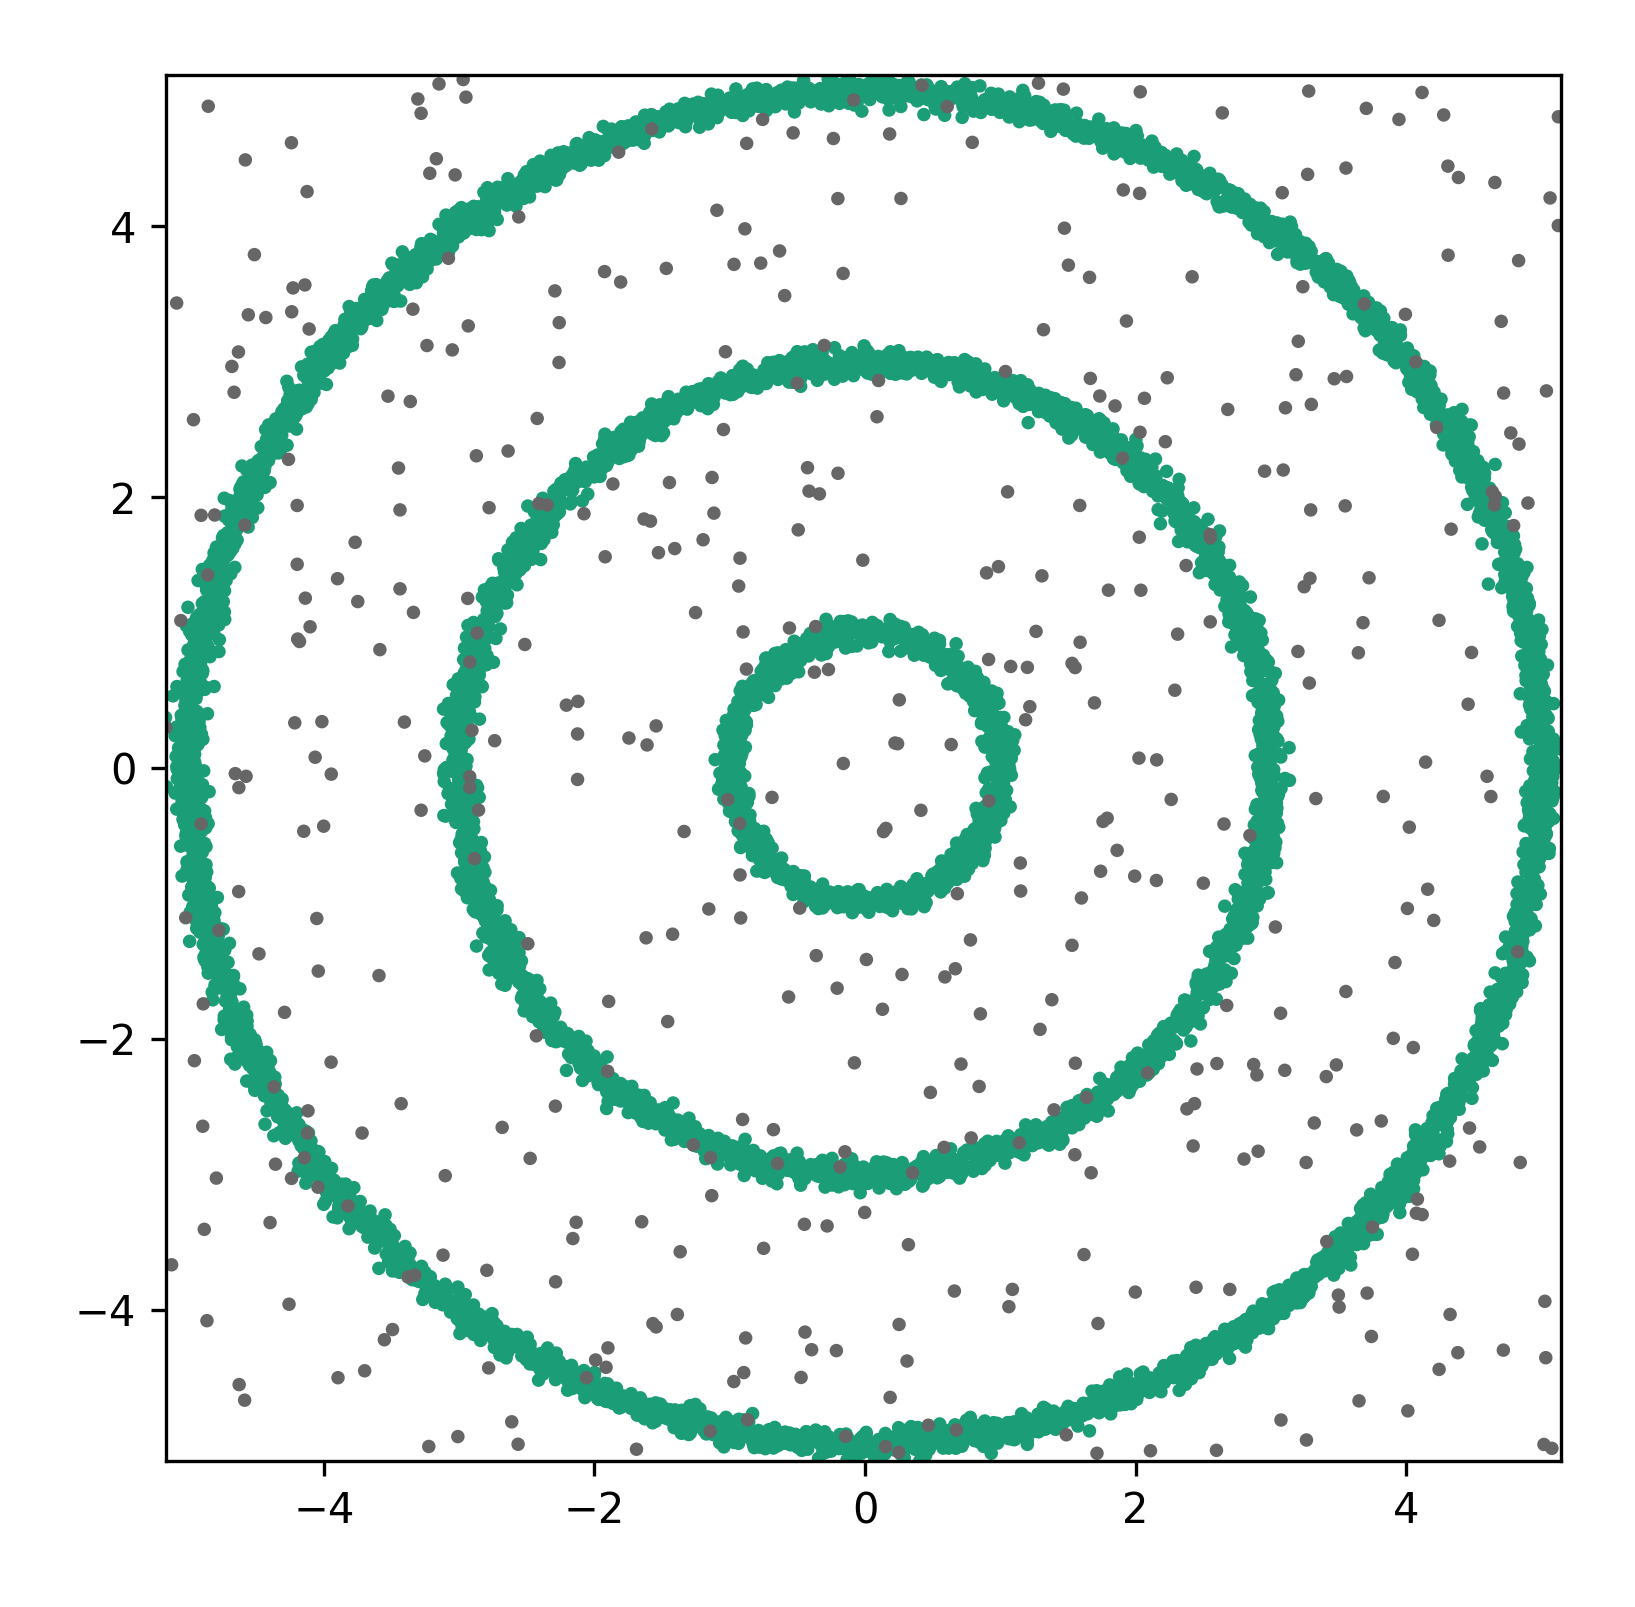
\includegraphics[width=2.5in]{static/bullseye.png}
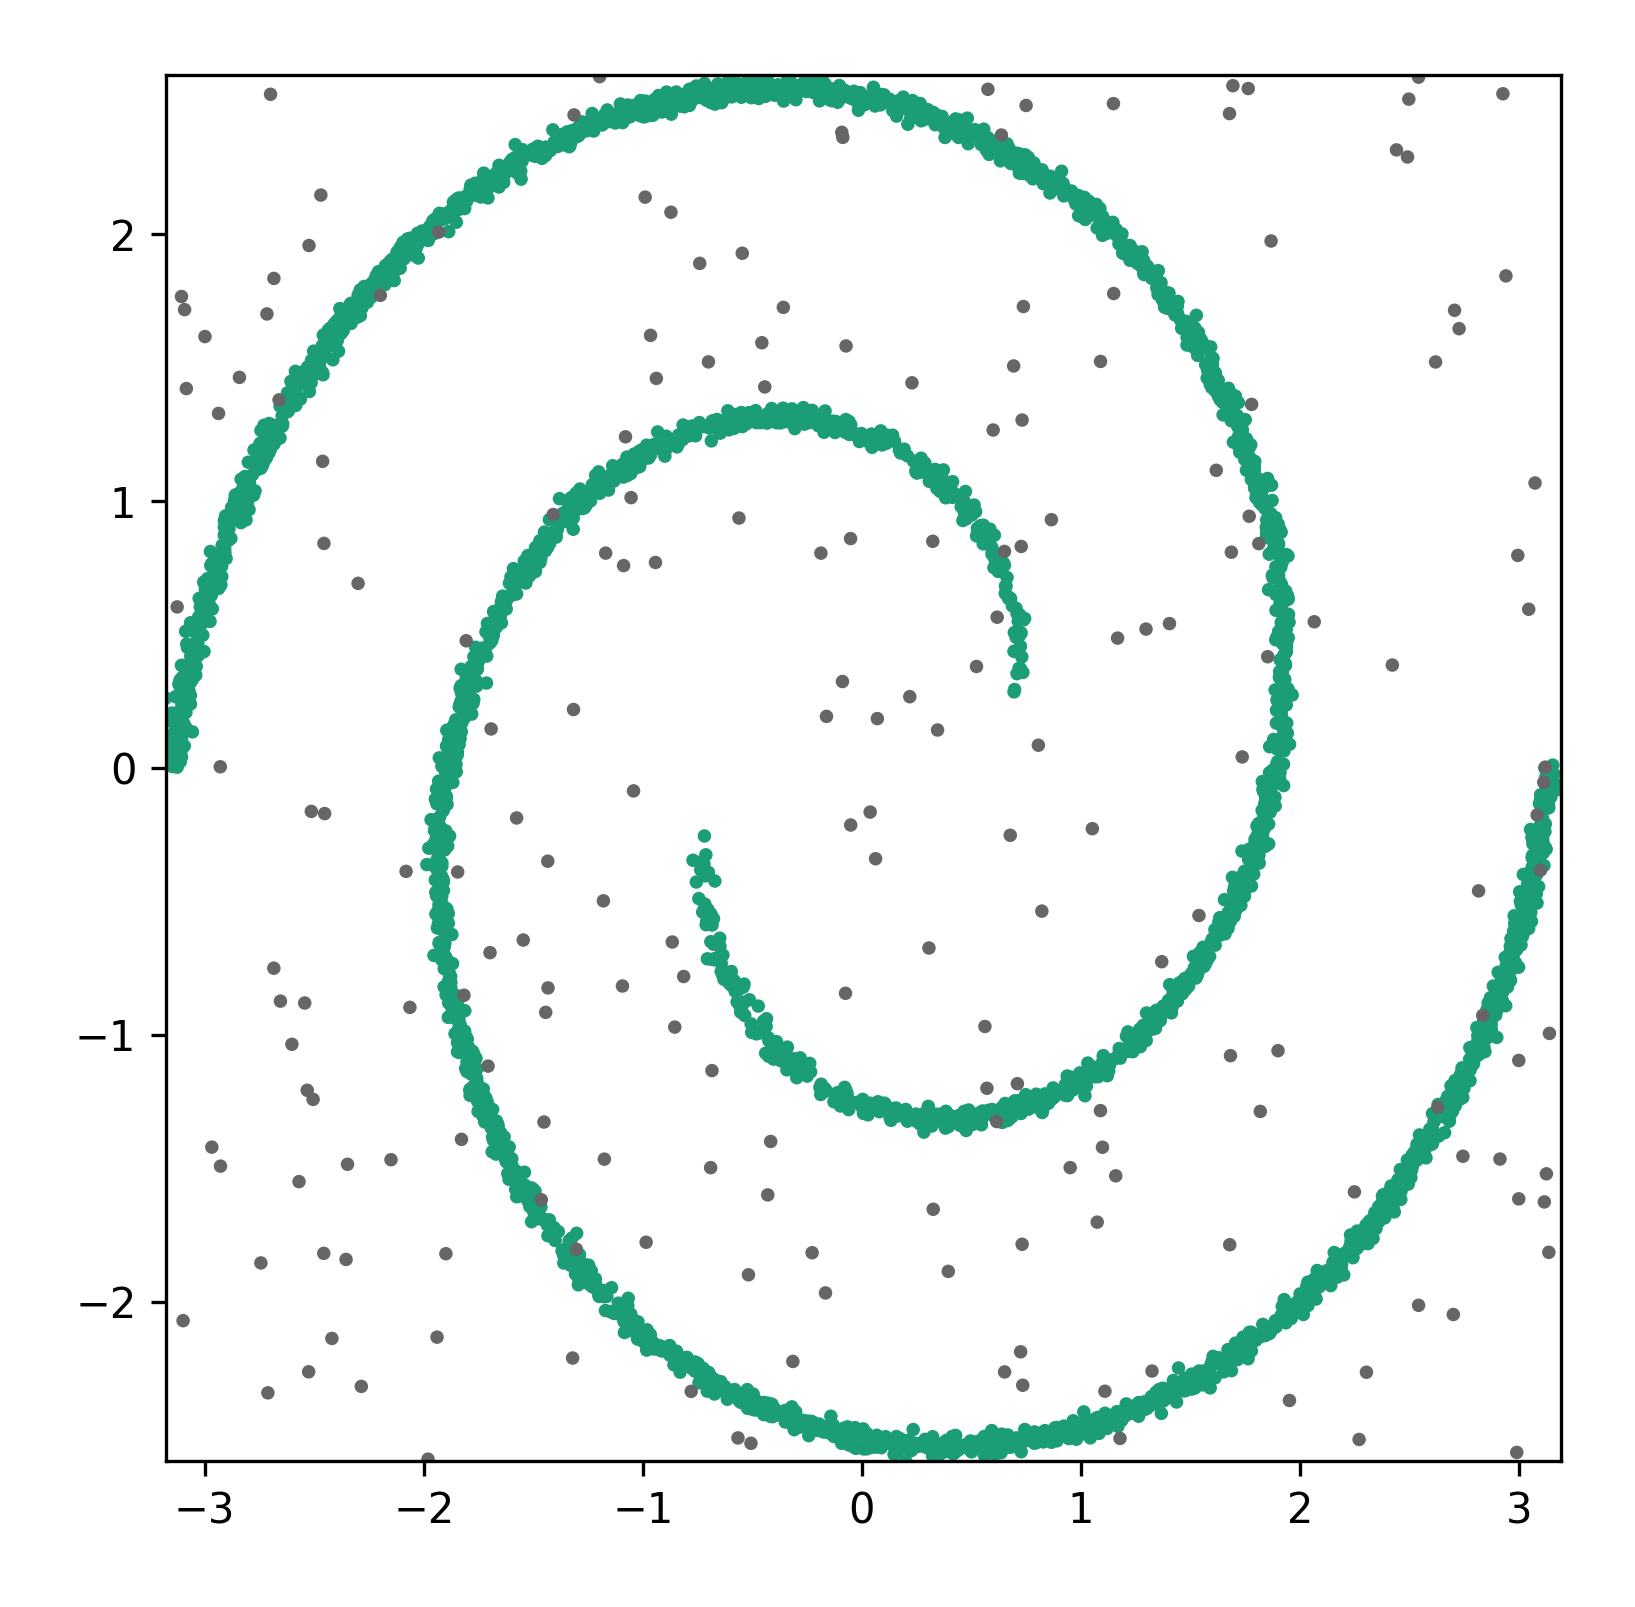
\includegraphics[width=2.5in]{static/spiral.png}
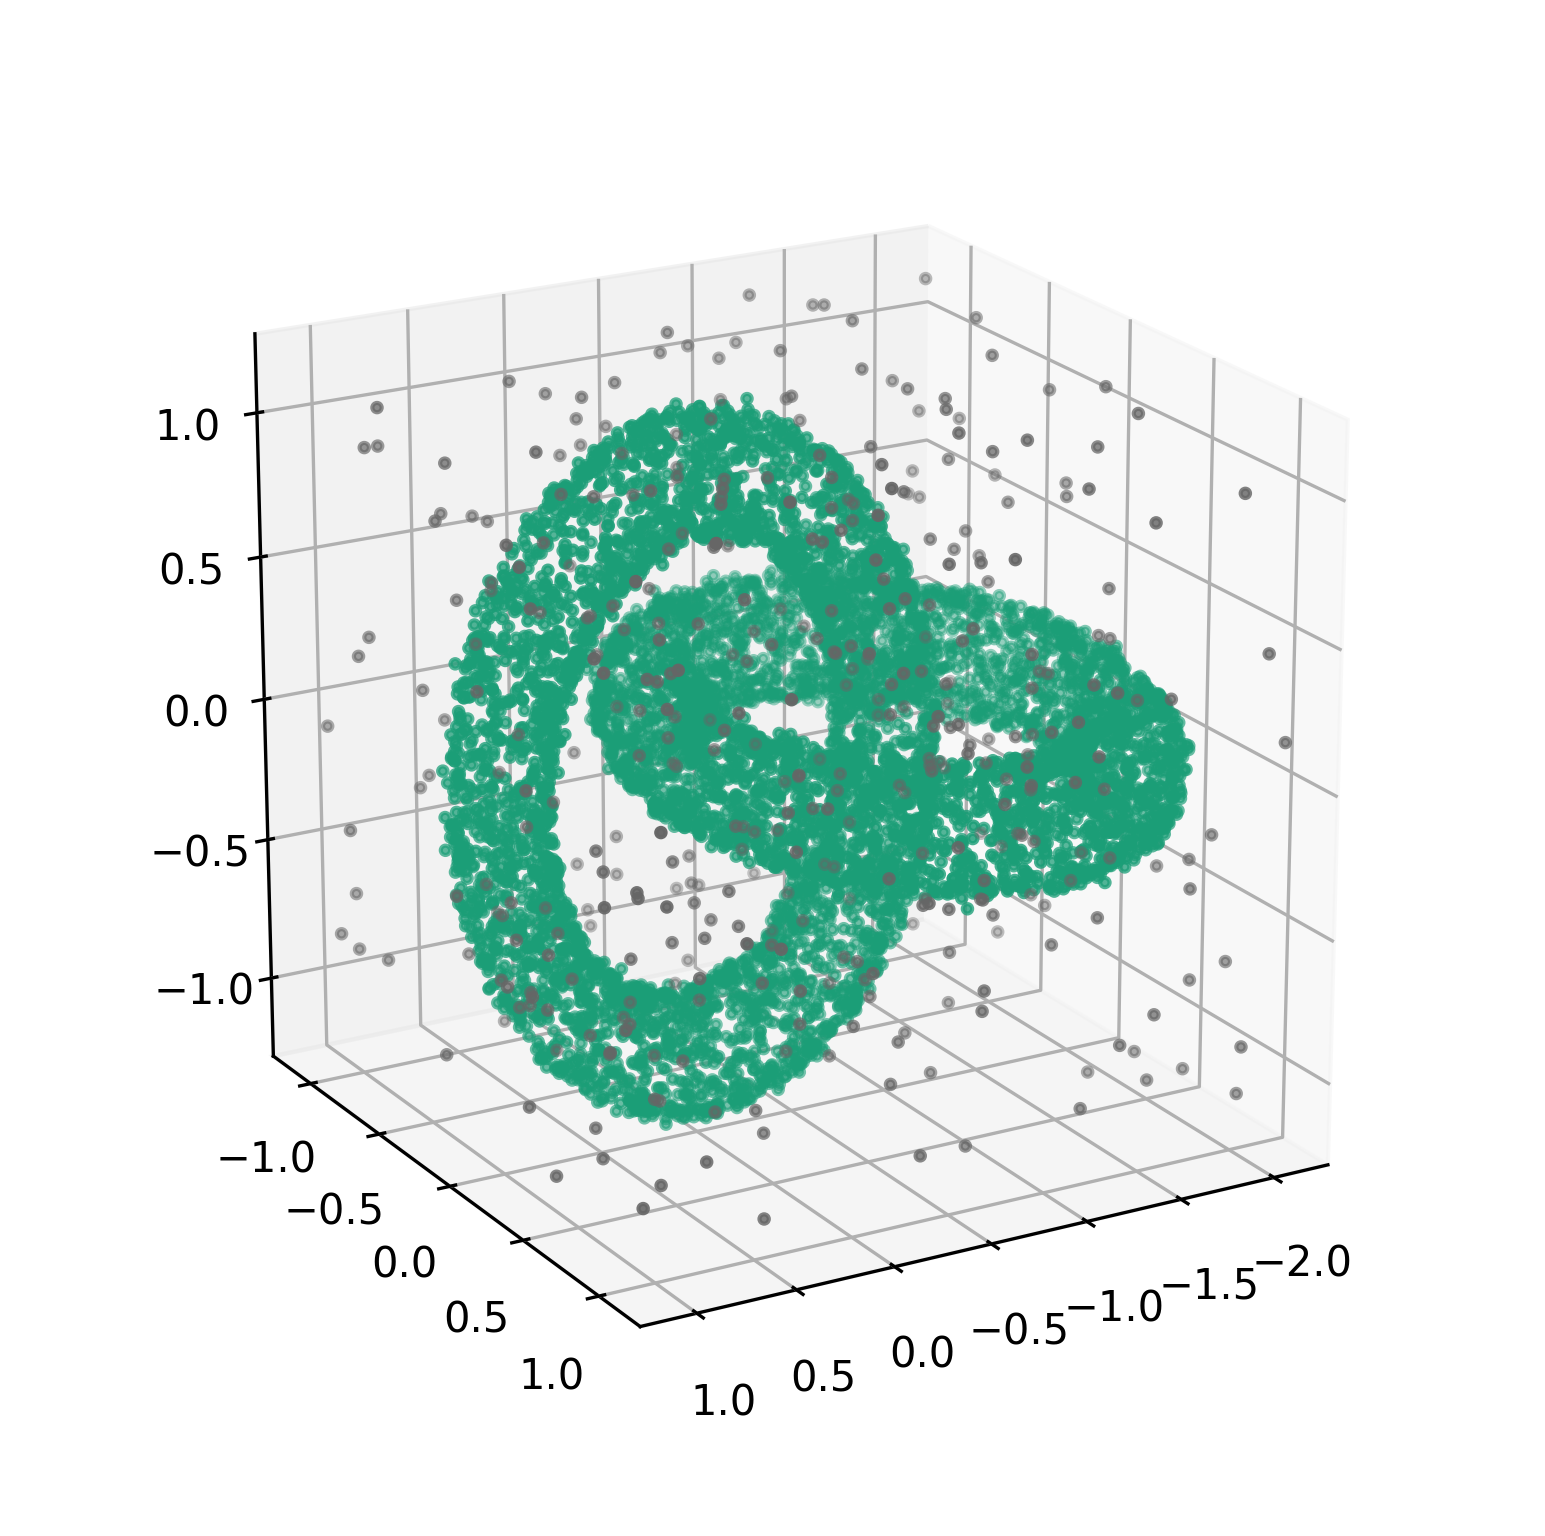
\includegraphics[width=3in]{static/interlocking_tori.png}
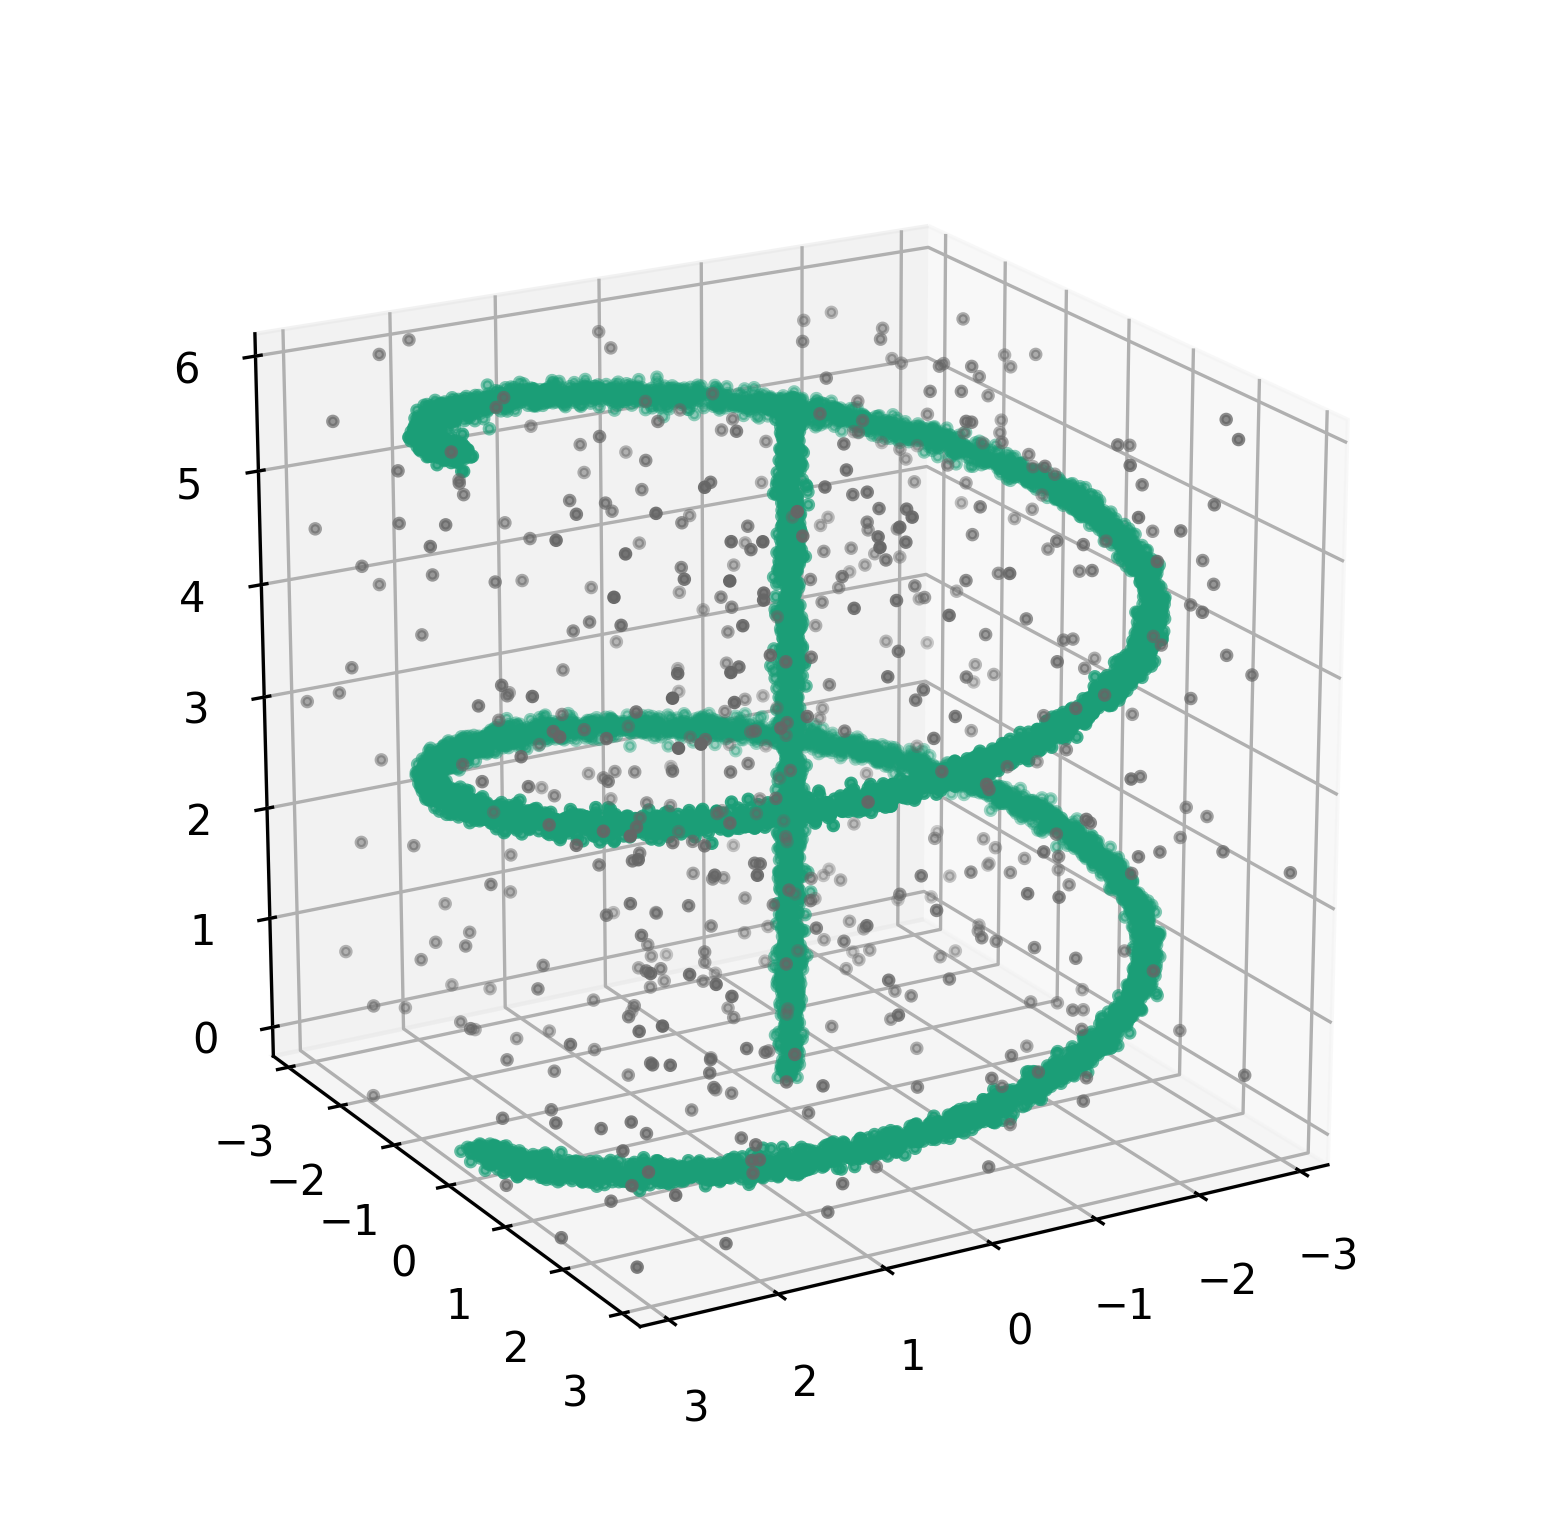
\includegraphics[width=3in]{static/skewer.png}
\caption{The Bullseye (top-left), Spiral (top-right), Interlocking Tori (bottom-left) and Skewer (bottom-left) datasets.}
\label{results:datasets}
\end{figure*}

For each dataset, we clustered using Manhattan, Euclidean, and Cosine distance functions.
Additionally, for this work, we allowed CLAM to cluster down until the manifold had thoroughly shattered.
We then iterated over all depths to compute the area under the ROC-Curve.

After computing anomalousness scores, we normalized each metric to a $[0, 1]$ range.
For each dataset, we present a confusion matrix, a ROC curve, and the area under the ROC curve for a sample of optimal depths. 
To demonstrate our methods are not overly-sensitive to depth we present all metrics in a 5-depth wide window.

Table~\ref{results:table} lists % TODO

\begin{table*}[!t]
\renewcommand{\arraystretch}{1.3}
\caption{Comparison of CHAODA with state-of-the-art algorithms}
\label{results:table}
\centering
\begin{tabular}{|c|c|c|c|c|c|c|c|c|c|c|c|c|c|c|c|}
\hline
{\textbf{Dataset}} & {\textbf{Metric}} & {\textbf{Method}} & \multicolumn{3}{c|}{\textbf{AUC ROC}} & \multicolumn{10}{c|}{\textbf{ }} \\
\hline
 &  &  & d - 2 & d & d + 2 &  &  &  &  &  &  &  &  &  & \\
\hline
\bfseries lympho & \bfseries cosine & \bfseries cluster\_cardinality & 0.926 & 0.949 & 0.838 &  &  &  &  &  &  &  &  &  & \\ 
\hline
\bfseries lympho & \bfseries cosine & \bfseries hierarchical & 0.927 & 0.940 & 0.938 &  &  &  &  &  &  &  &  &  & \\ 
\hline
\bfseries lympho & \bfseries cosine & \bfseries k\_neighborhood & 0.500 & 0.888 & 0.725 &  &  &  &  &  &  &  &  &  & \\ 
\hline
\bfseries lympho & \bfseries cosine & \bfseries random\_walk & 0.803 & 0.964 & 0.952 &  &  &  &  &  &  &  &  &  & \\ 
\hline
\bfseries lympho & \bfseries cosine & \bfseries subgraph\_cardinality & 0.583 & 0.739 & 0.729 &  &  &  &  &  &  &  &  &  & \\ 
\hline
\bfseries lympho & \bfseries euclidean & \bfseries cluster\_cardinality & 0.672 & 0.904 & 0.887 &  &  &  &  &  &  &  &  &  & \\ 
\hline
\bfseries lympho & \bfseries euclidean & \bfseries hierarchical & 0.672 & 0.869 & 0.863 &  &  &  &  &  &  &  &  &  & \\ 
\hline
\bfseries lympho & \bfseries euclidean & \bfseries k\_neighborhood & 0.500 & 0.573 & 0.500 &  &  &  &  &  &  &  &  &  & \\ 
\hline
\bfseries lympho & \bfseries euclidean & \bfseries random\_walk & 0.704 & 0.783 & 0.692 &  &  &  &  &  &  &  &  &  & \\ 
\hline
\bfseries lympho & \bfseries euclidean & \bfseries subgraph\_cardinality & 0.500 & 0.500 & 0.500 &  &  &  &  &  &  &  &  &  & \\ 
\hline
\bfseries lympho & \bfseries manhattan & \bfseries cluster\_cardinality & 0.793 & 0.965 & 0.962 &  &  &  &  &  &  &  &  &  & \\ 
\hline
\bfseries lympho & \bfseries manhattan & \bfseries hierarchical & 0.935 & 0.965 & 0.955 &  &  &  &  &  &  &  &  &  & \\ 
\hline
\bfseries lympho & \bfseries manhattan & \bfseries k\_neighborhood & 0.648 & 0.818 & 0.818 &  &  &  &  &  &  &  &  &  & \\ 
\hline
\bfseries lympho & \bfseries manhattan & \bfseries random\_walk & 0.763 & 0.960 & 0.955 &  &  &  &  &  &  &  &  &  & \\ 
\hline
\bfseries lympho & \bfseries manhattan & \bfseries subgraph\_cardinality & 0.583 & 0.663 & 0.660 &  &  &  &  &  &  &  &  &  & \\ 
\hline

\end{tabular}
\end{table*}

\begin{figure*}[!t]
\centering
% Annthyroid
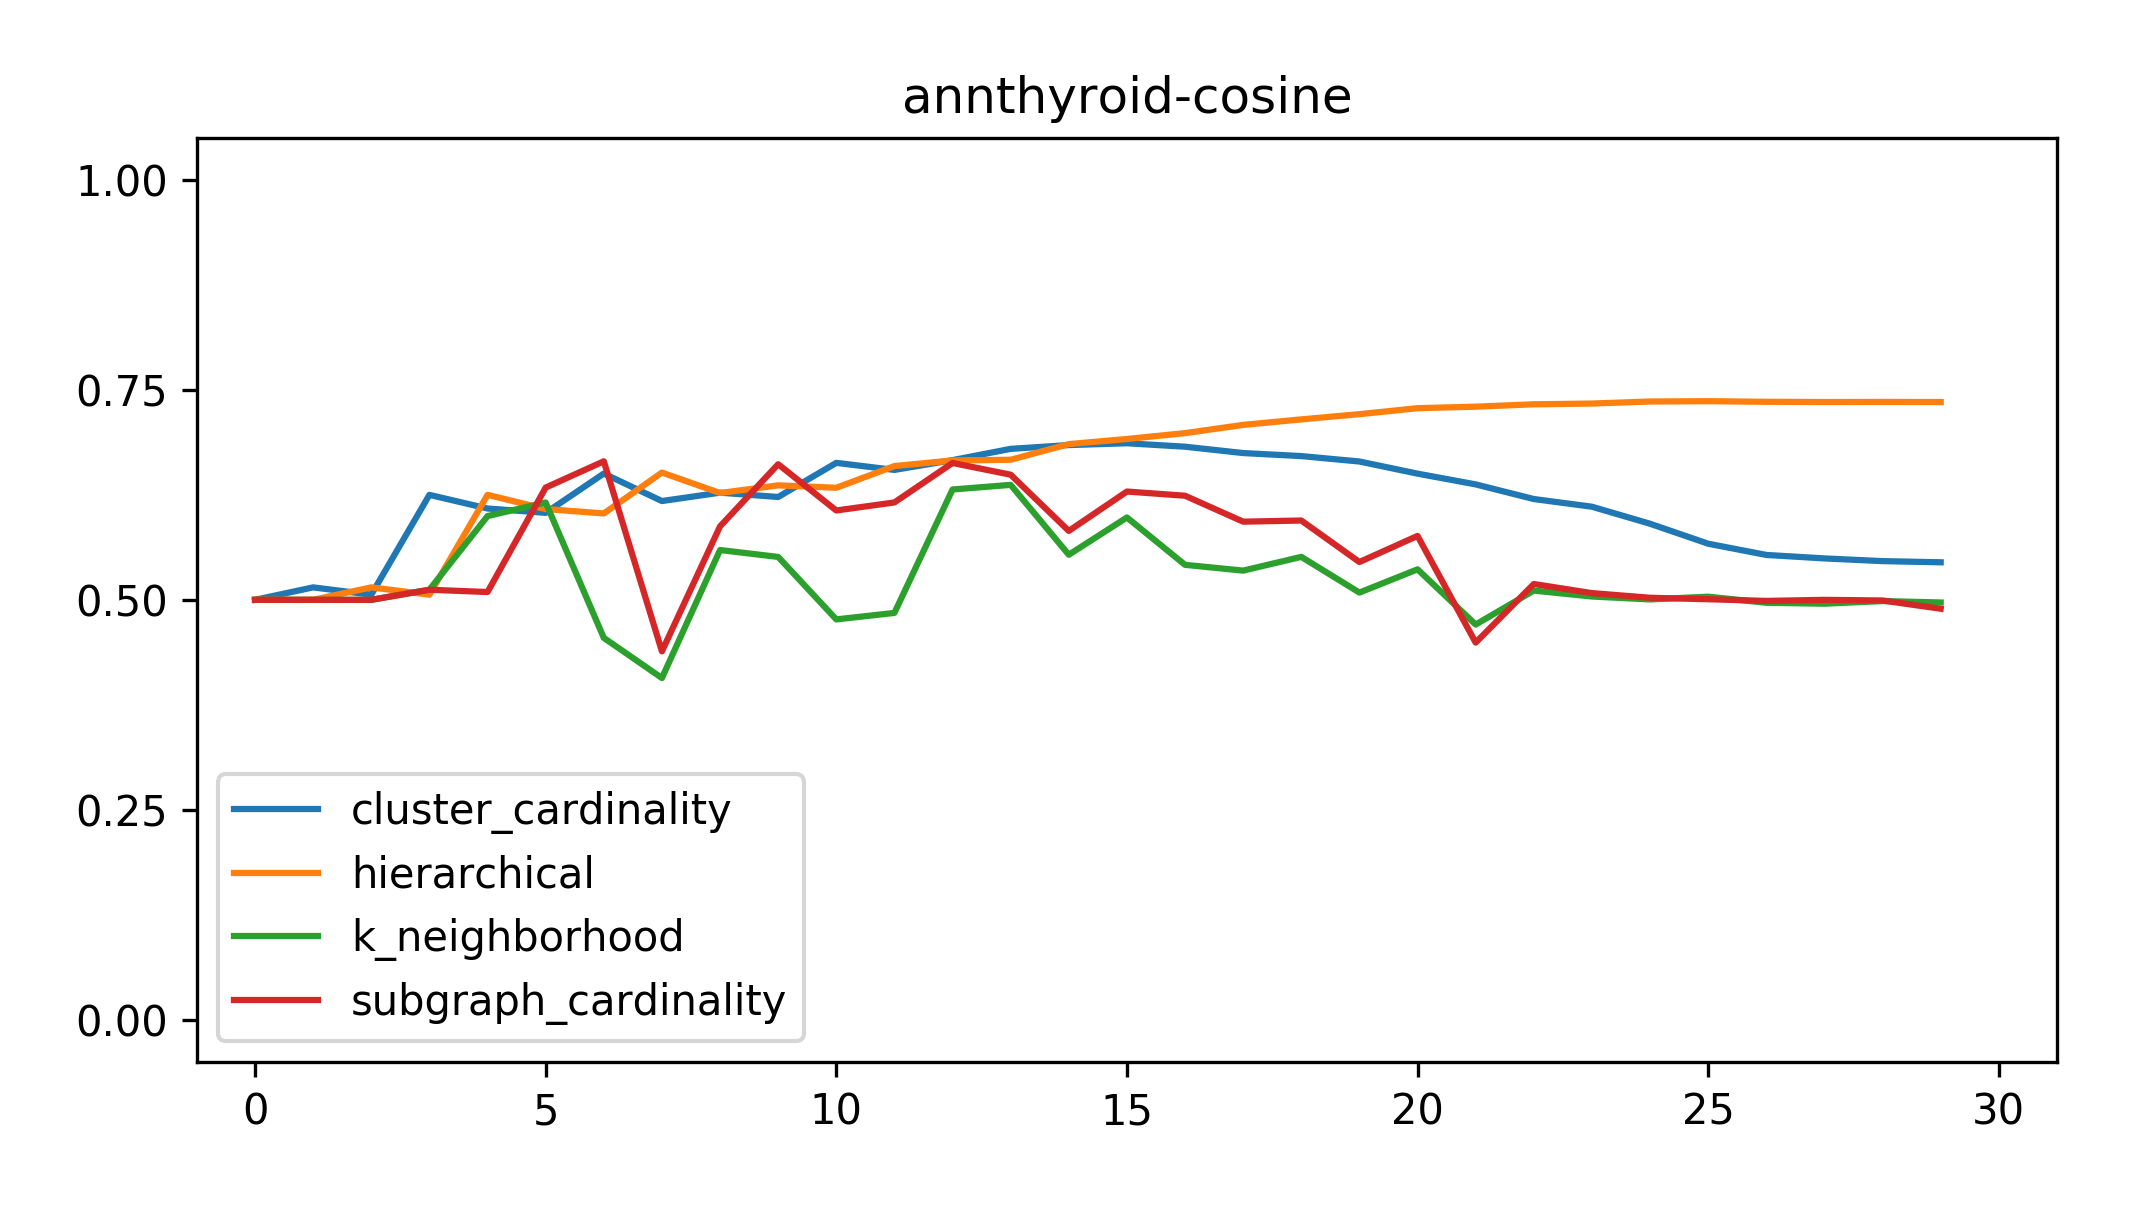
\includegraphics[width=2.2in]{kdd/static/auc_vs_depth/annthyroid-cosine.png}
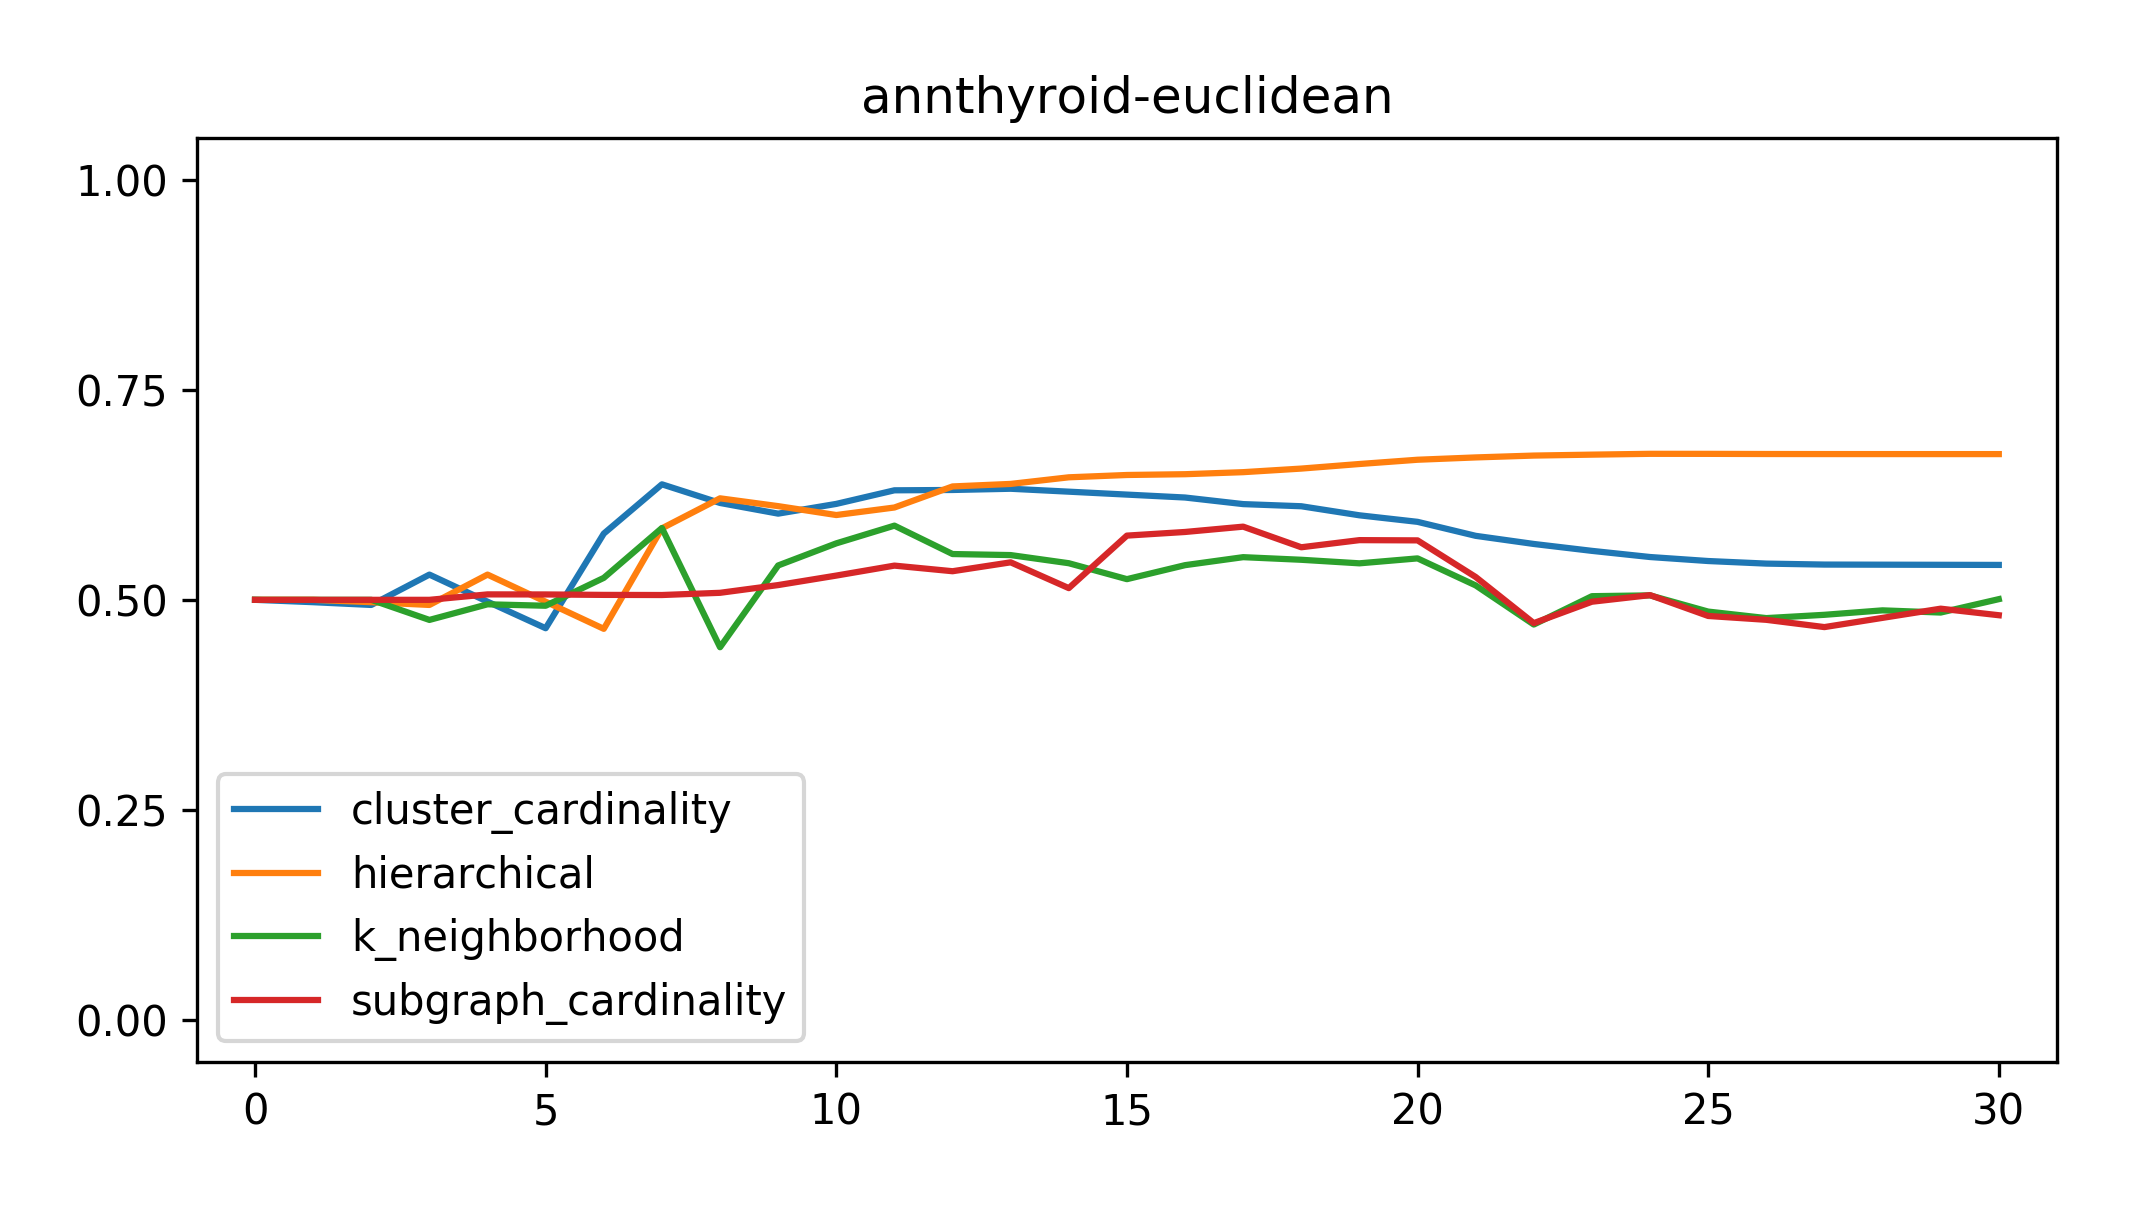
\includegraphics[width=2.2in]{kdd/static/auc_vs_depth/annthyroid-euclidean.png}
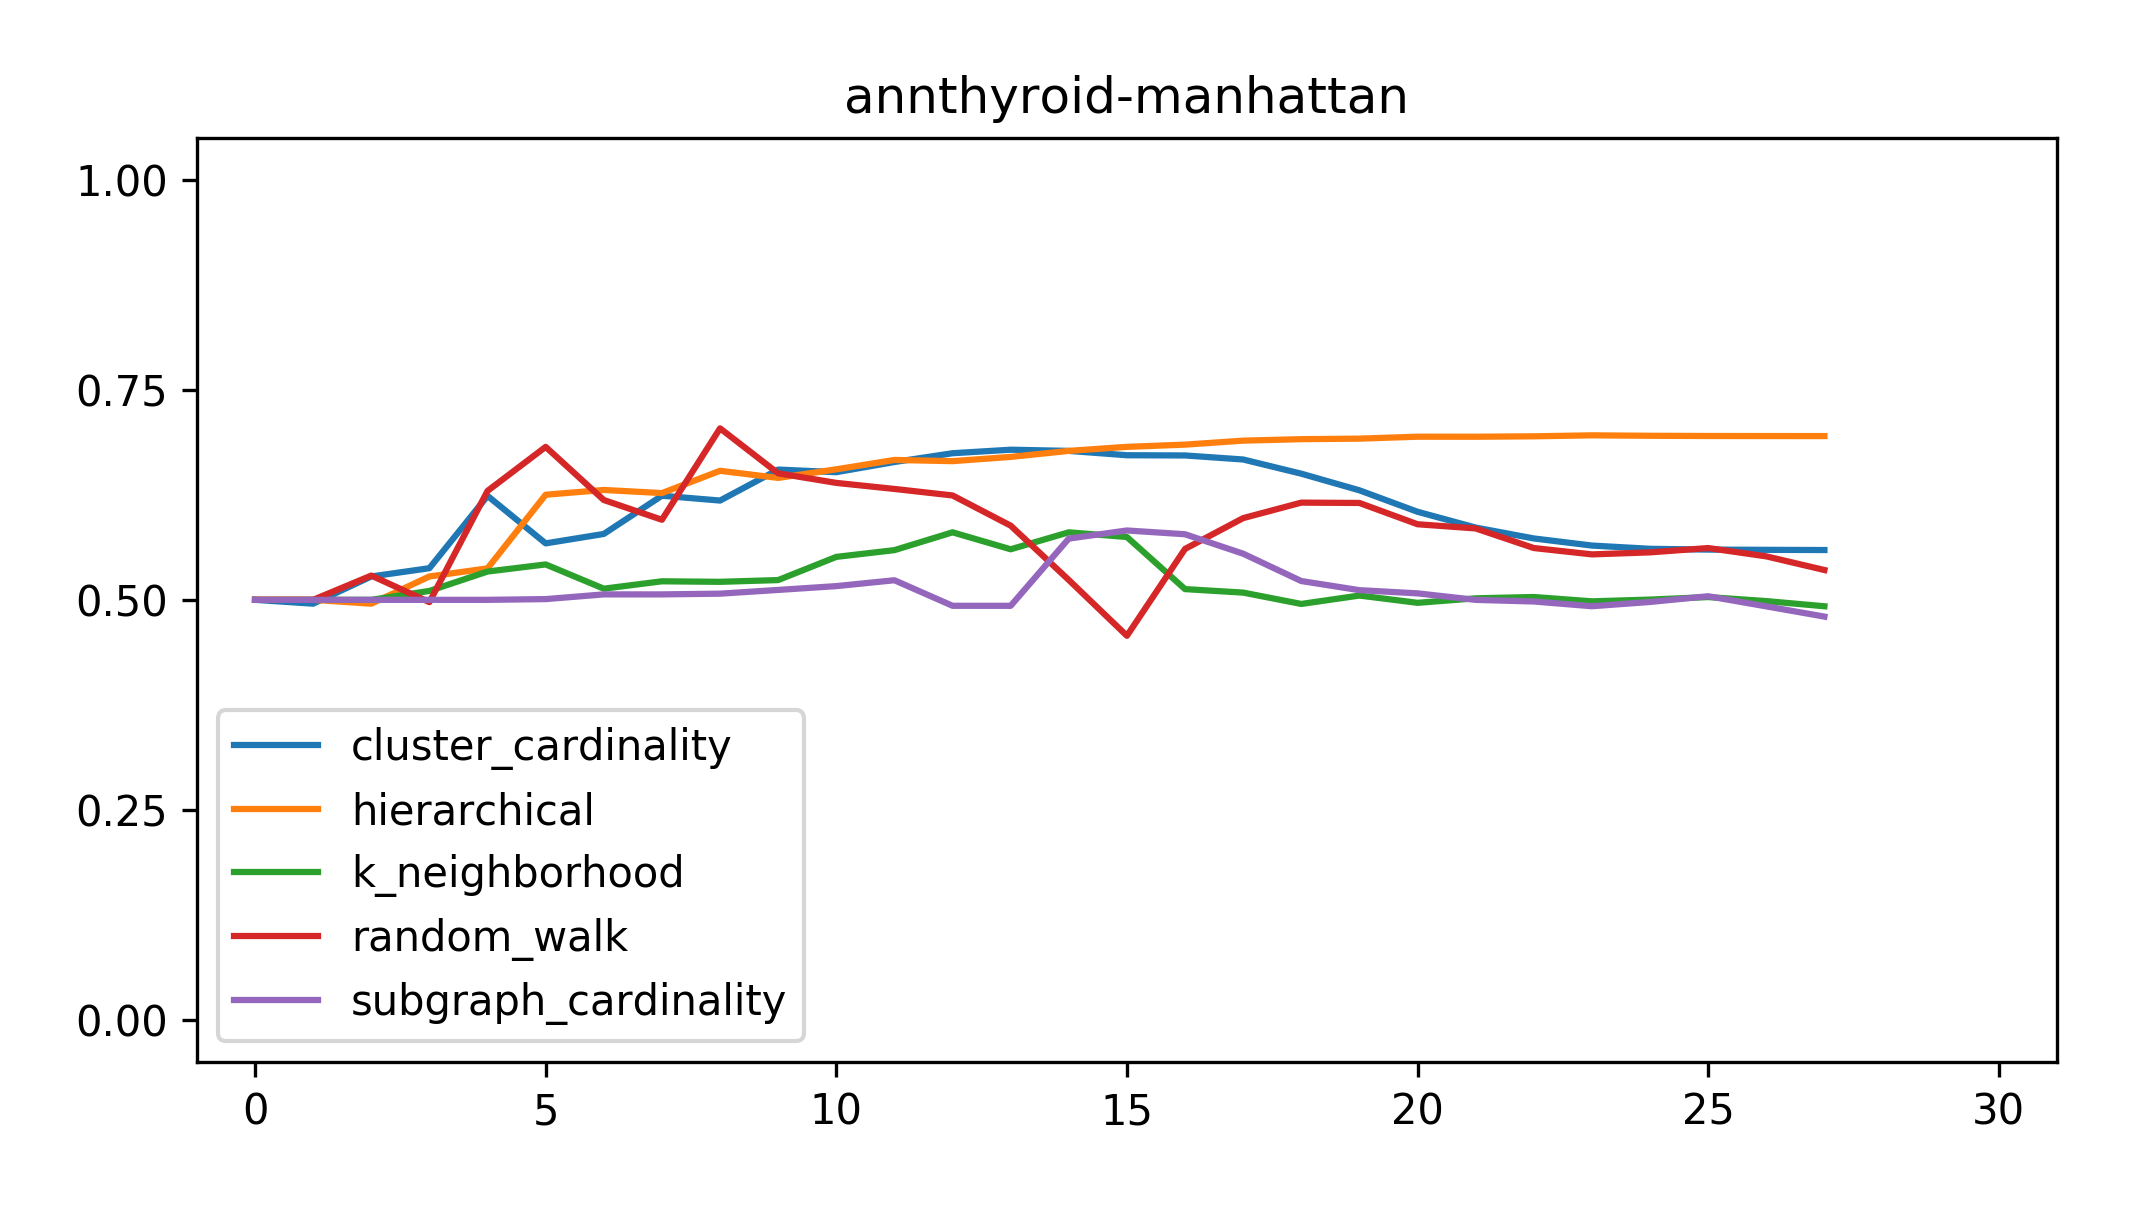
\includegraphics[width=2.2in]{kdd/static/auc_vs_depth/annthyroid-manhattan.png}

% Arrhythmia
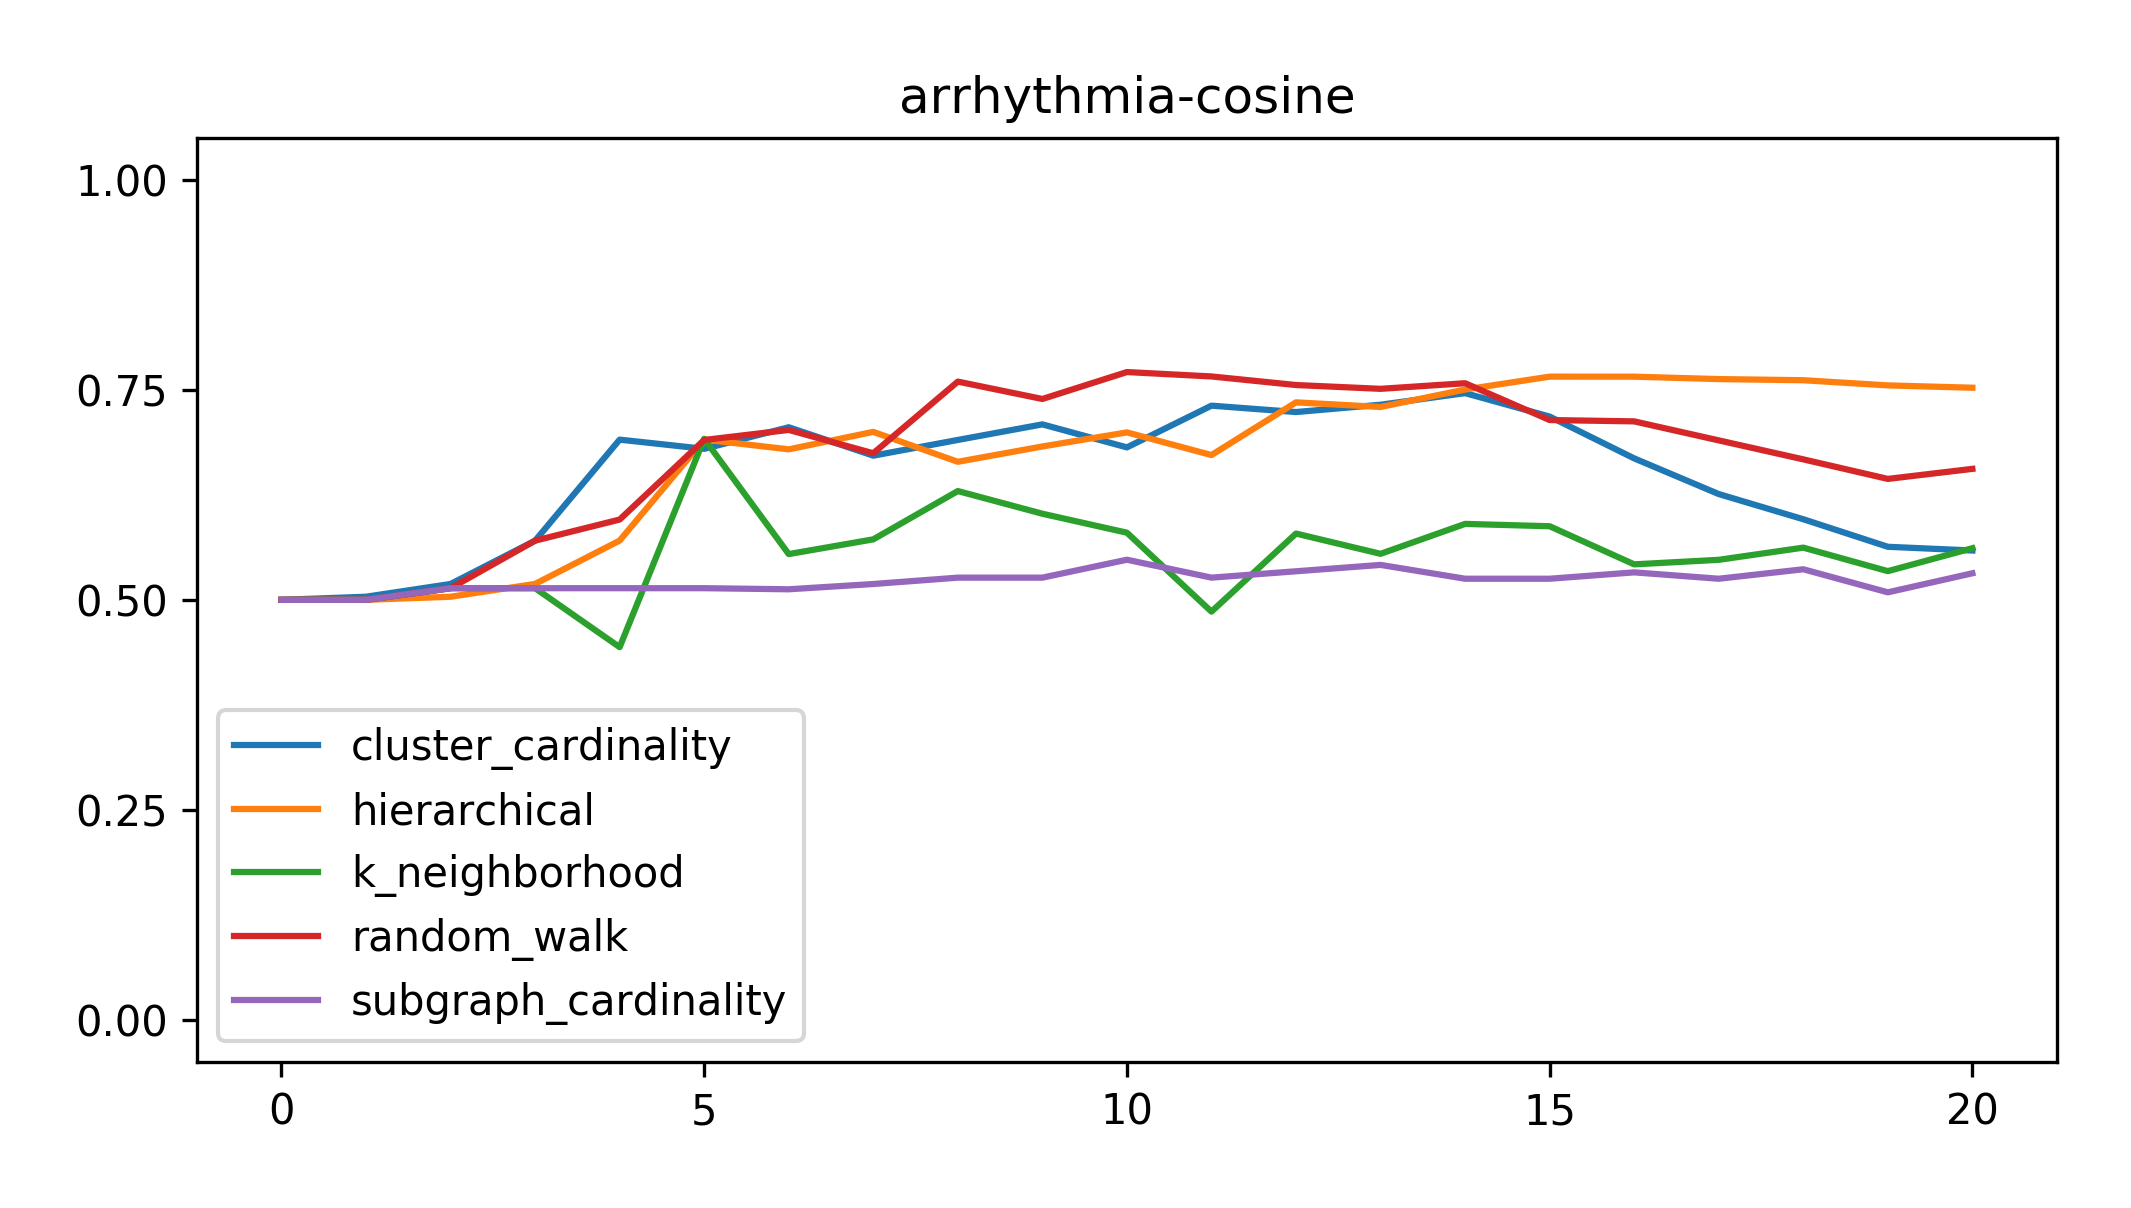
\includegraphics[width=2.2in]{kdd/static/auc_vs_depth/arrhythmia-cosine.png}
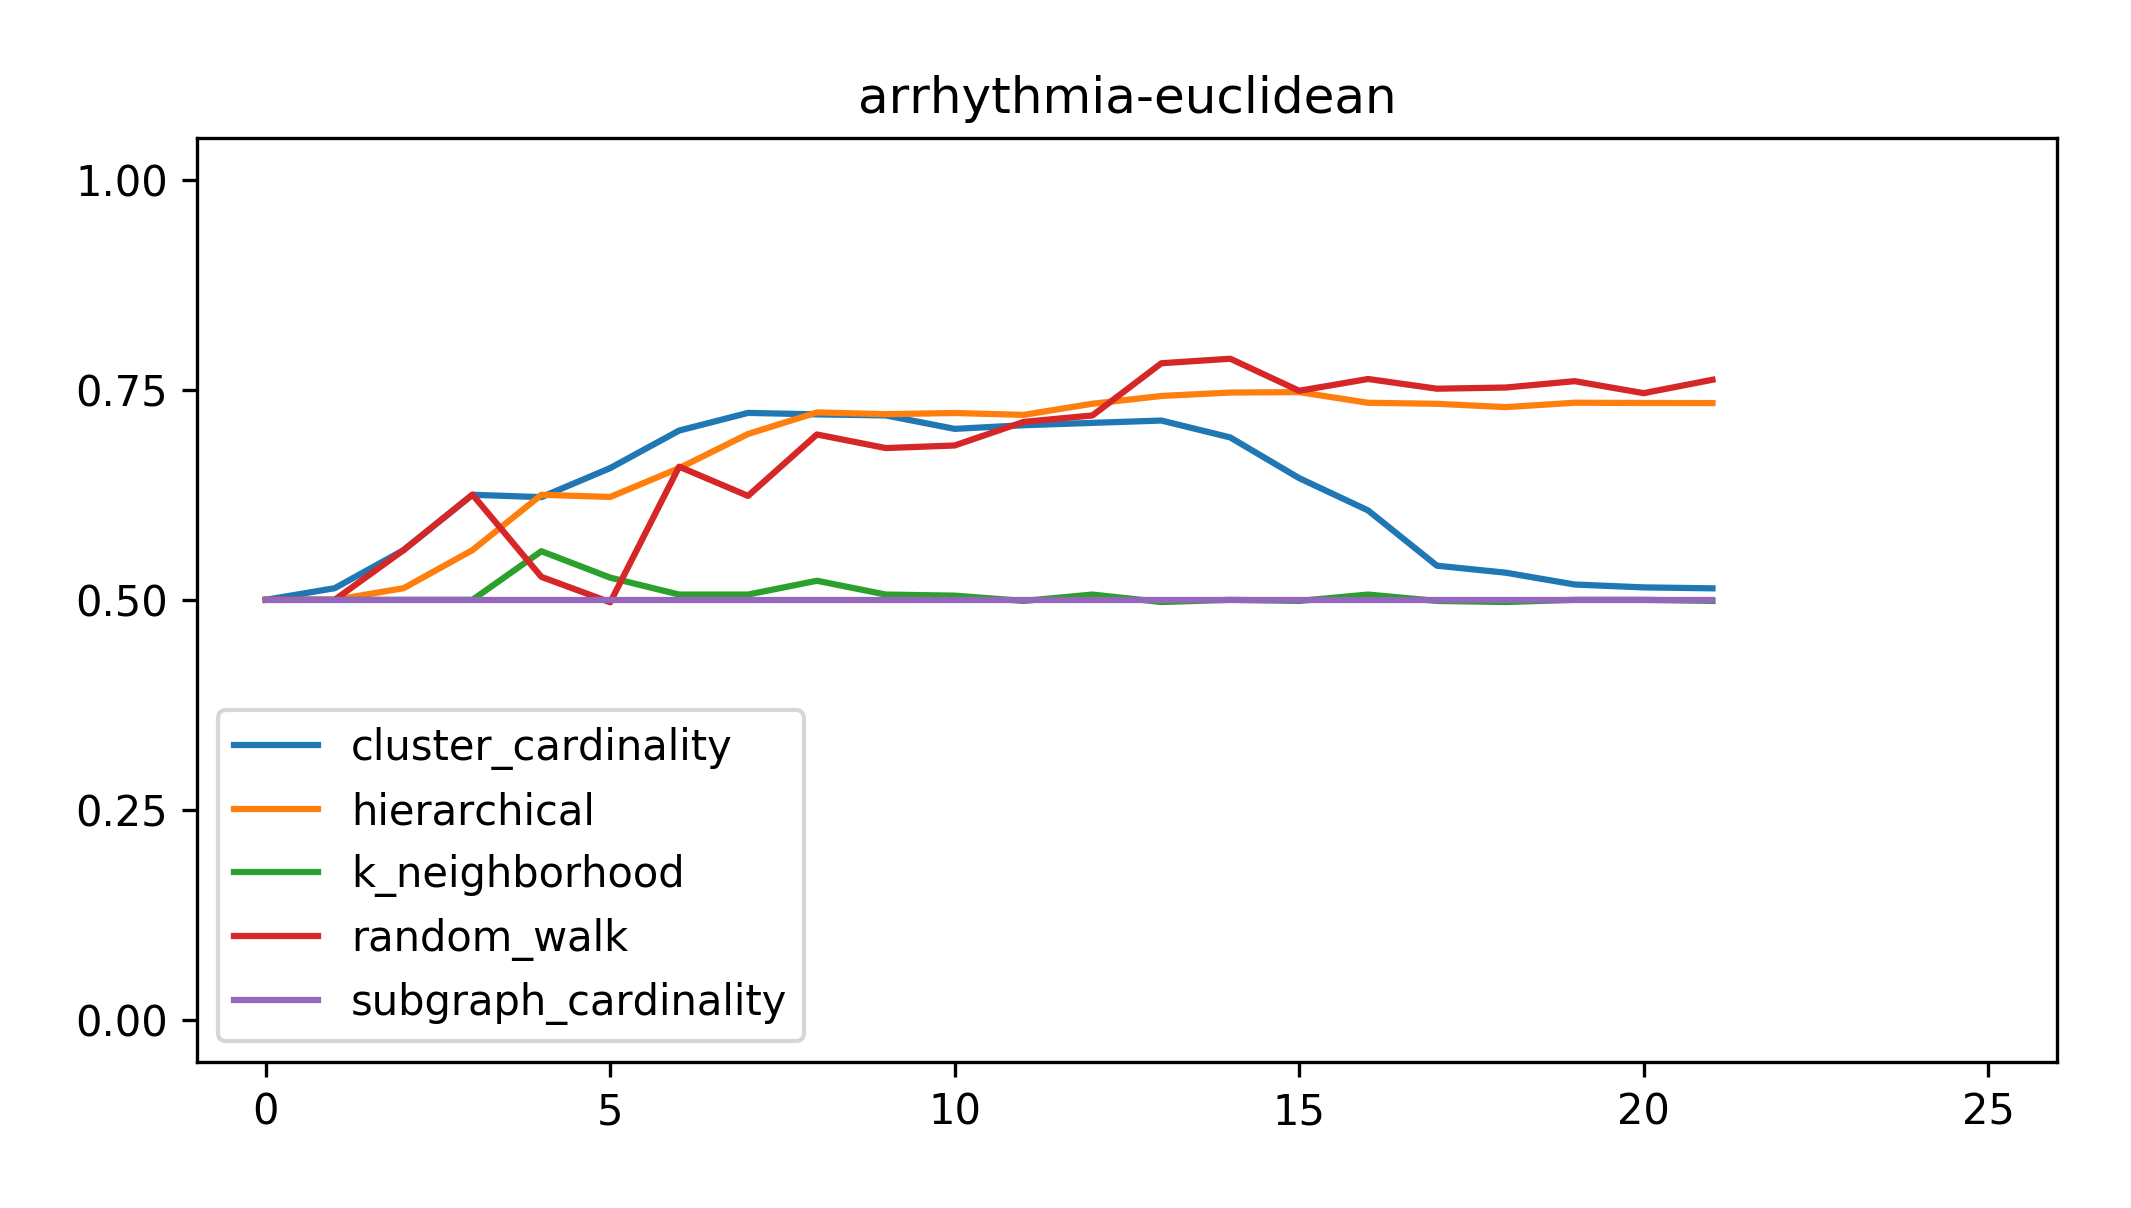
\includegraphics[width=2.2in]{kdd/static/auc_vs_depth/arrhythmia-euclidean.png}
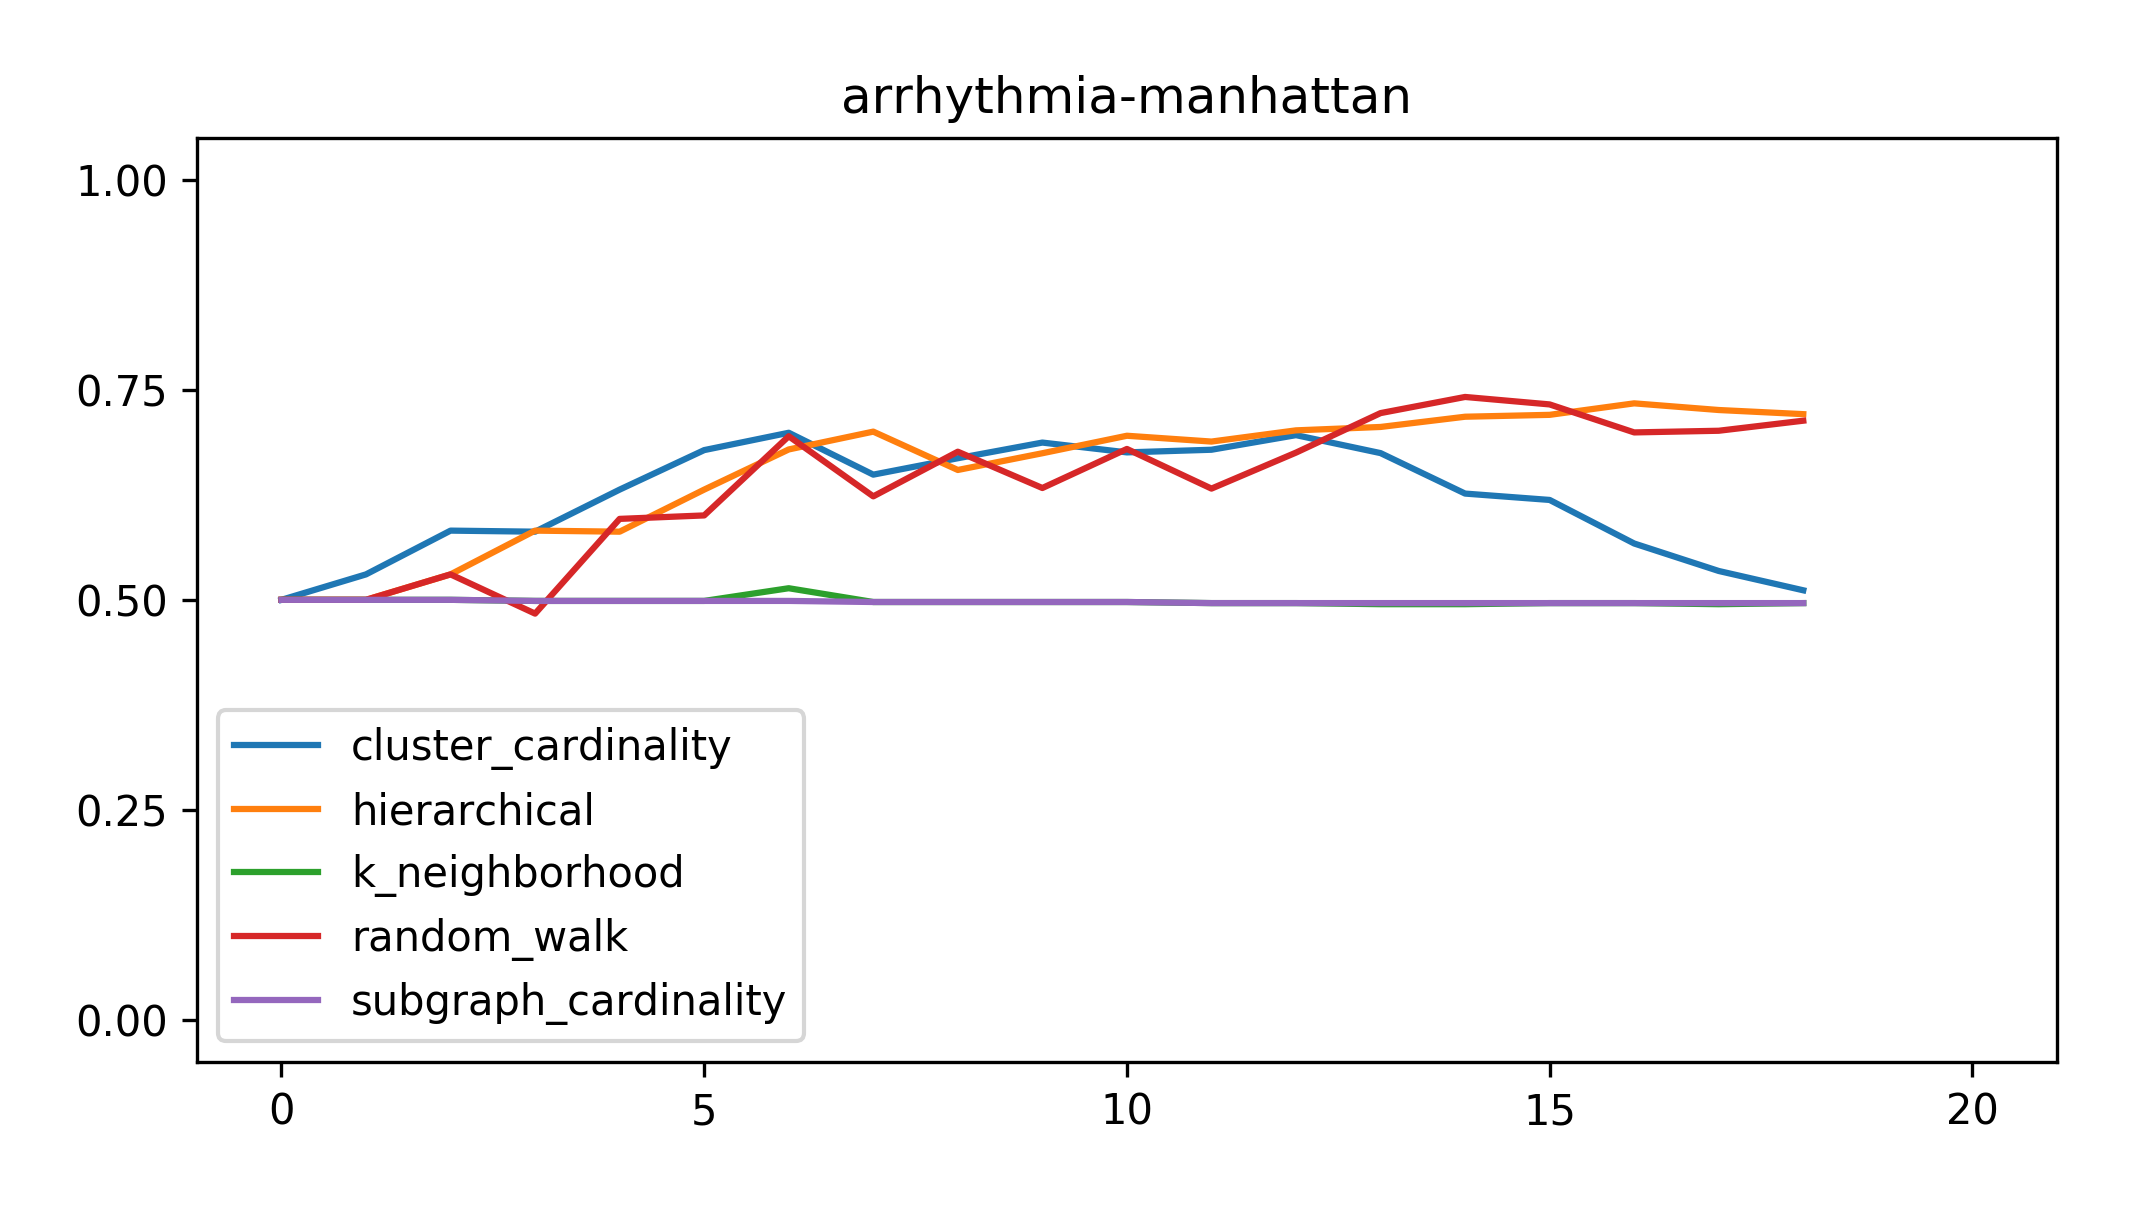
\includegraphics[width=2.2in]{kdd/static/auc_vs_depth/arrhythmia-manhattan.png}

% BreastW
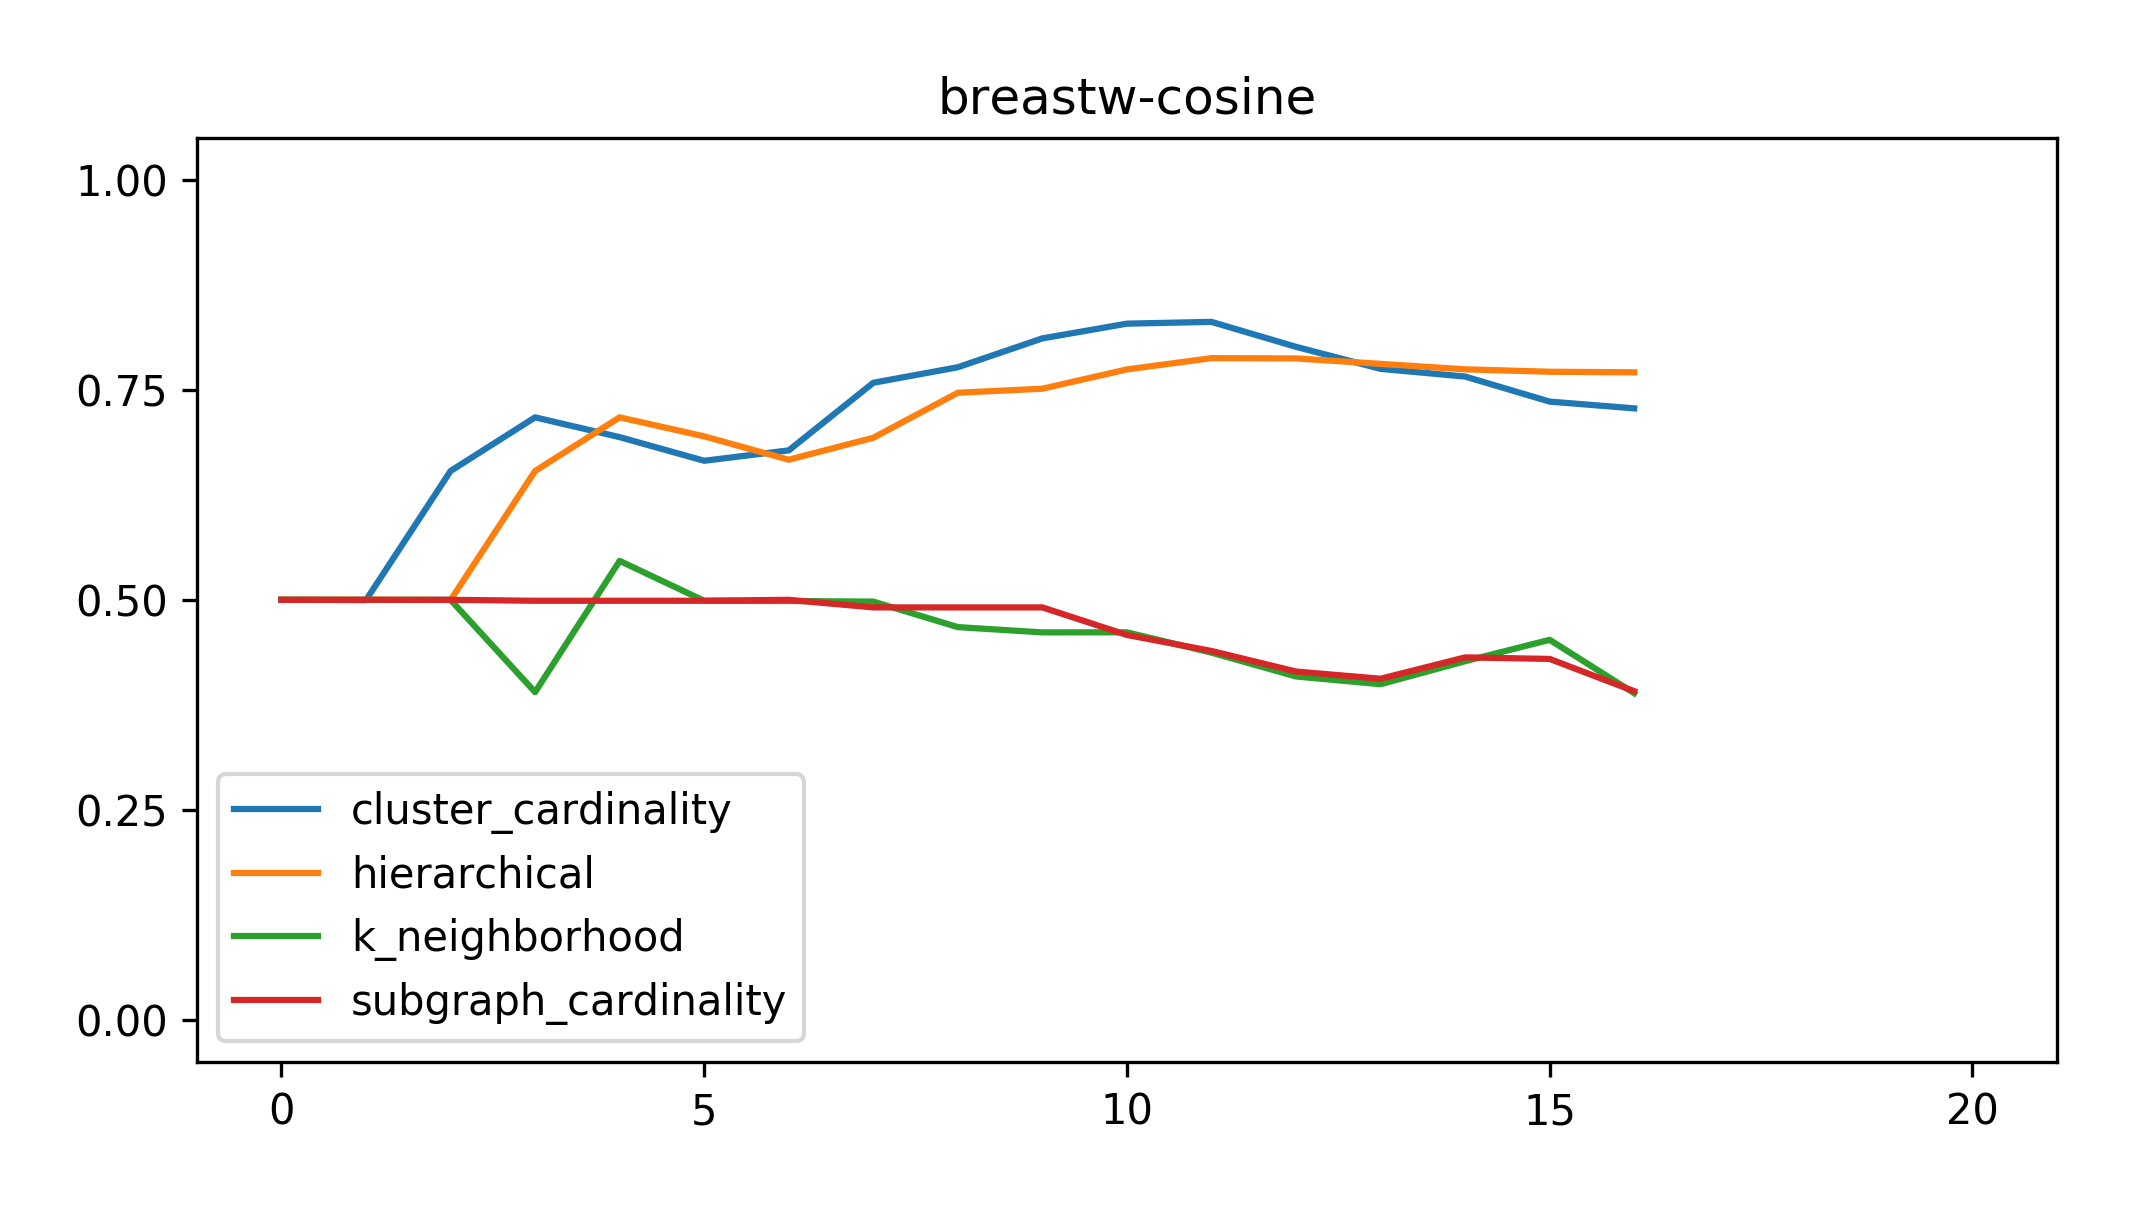
\includegraphics[width=2.2in]{kdd/static/auc_vs_depth/breastw-cosine.png}
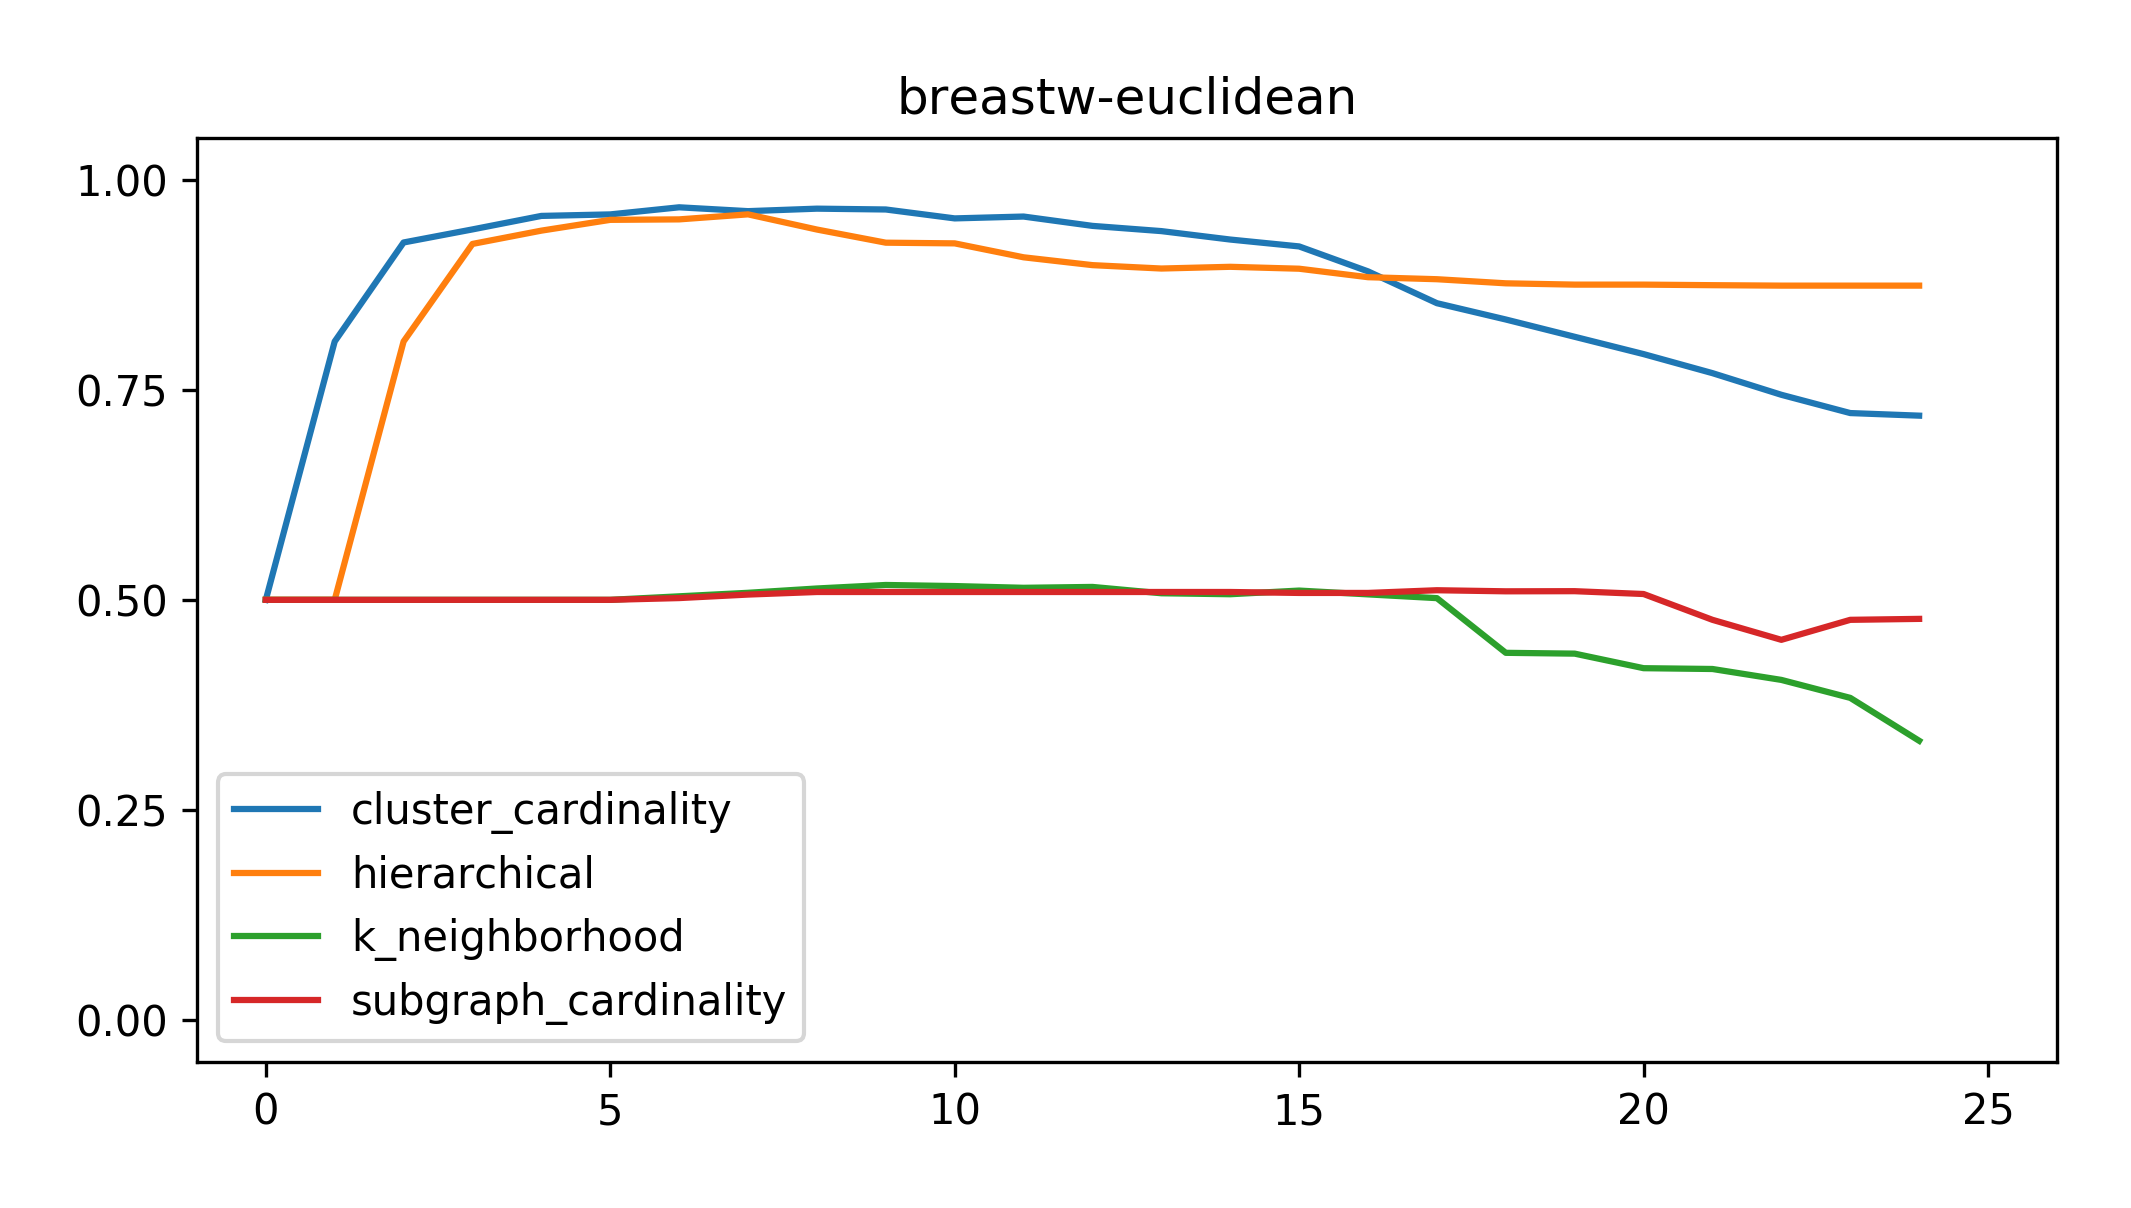
\includegraphics[width=2.2in]{kdd/static/auc_vs_depth/breastw-euclidean.png}
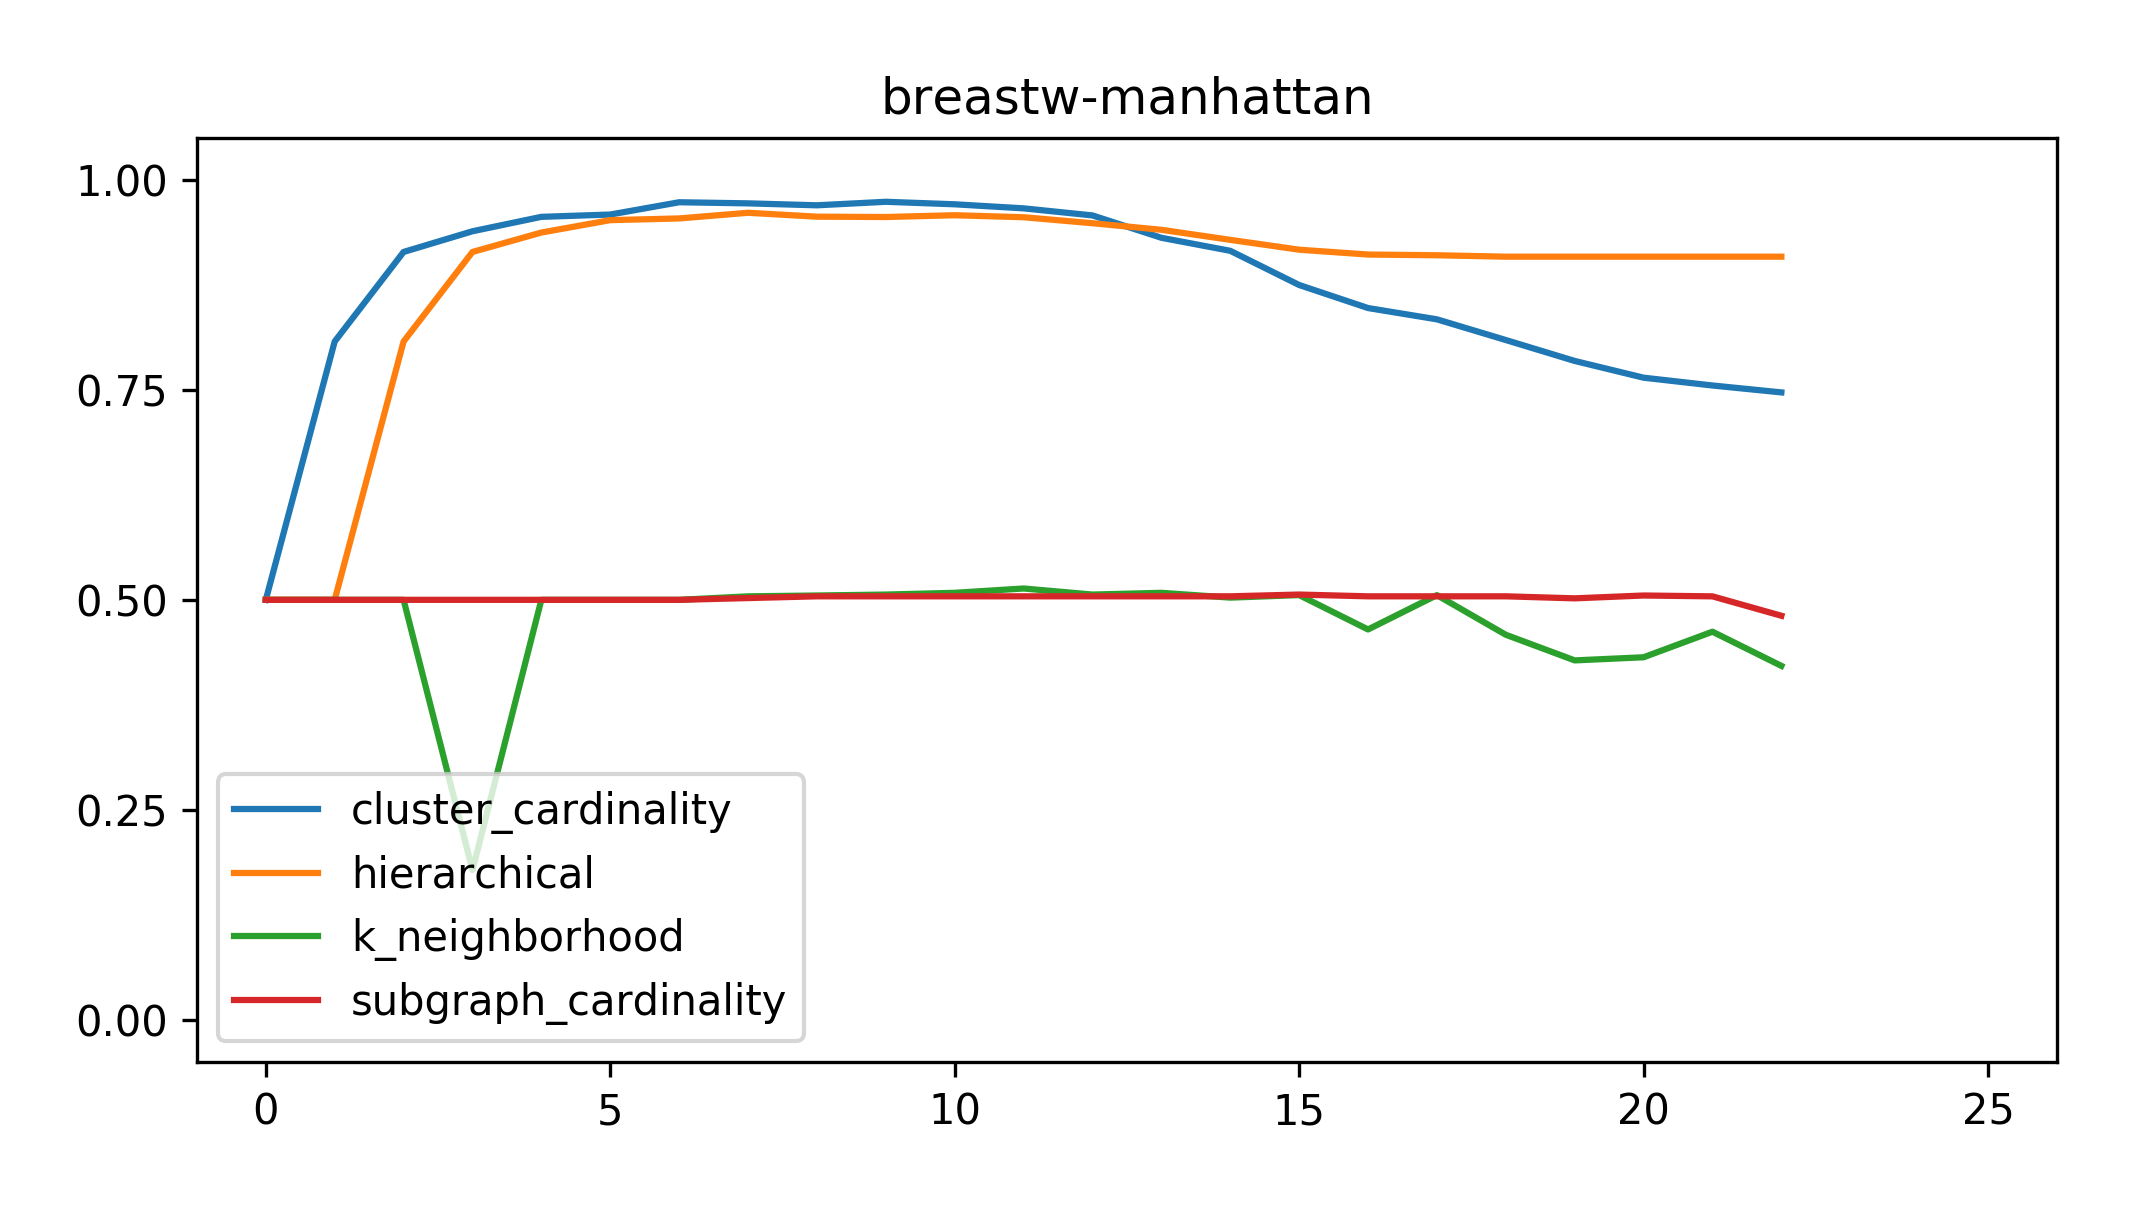
\includegraphics[width=2.2in]{kdd/static/auc_vs_depth/breastw-manhattan.png}

% Cardio
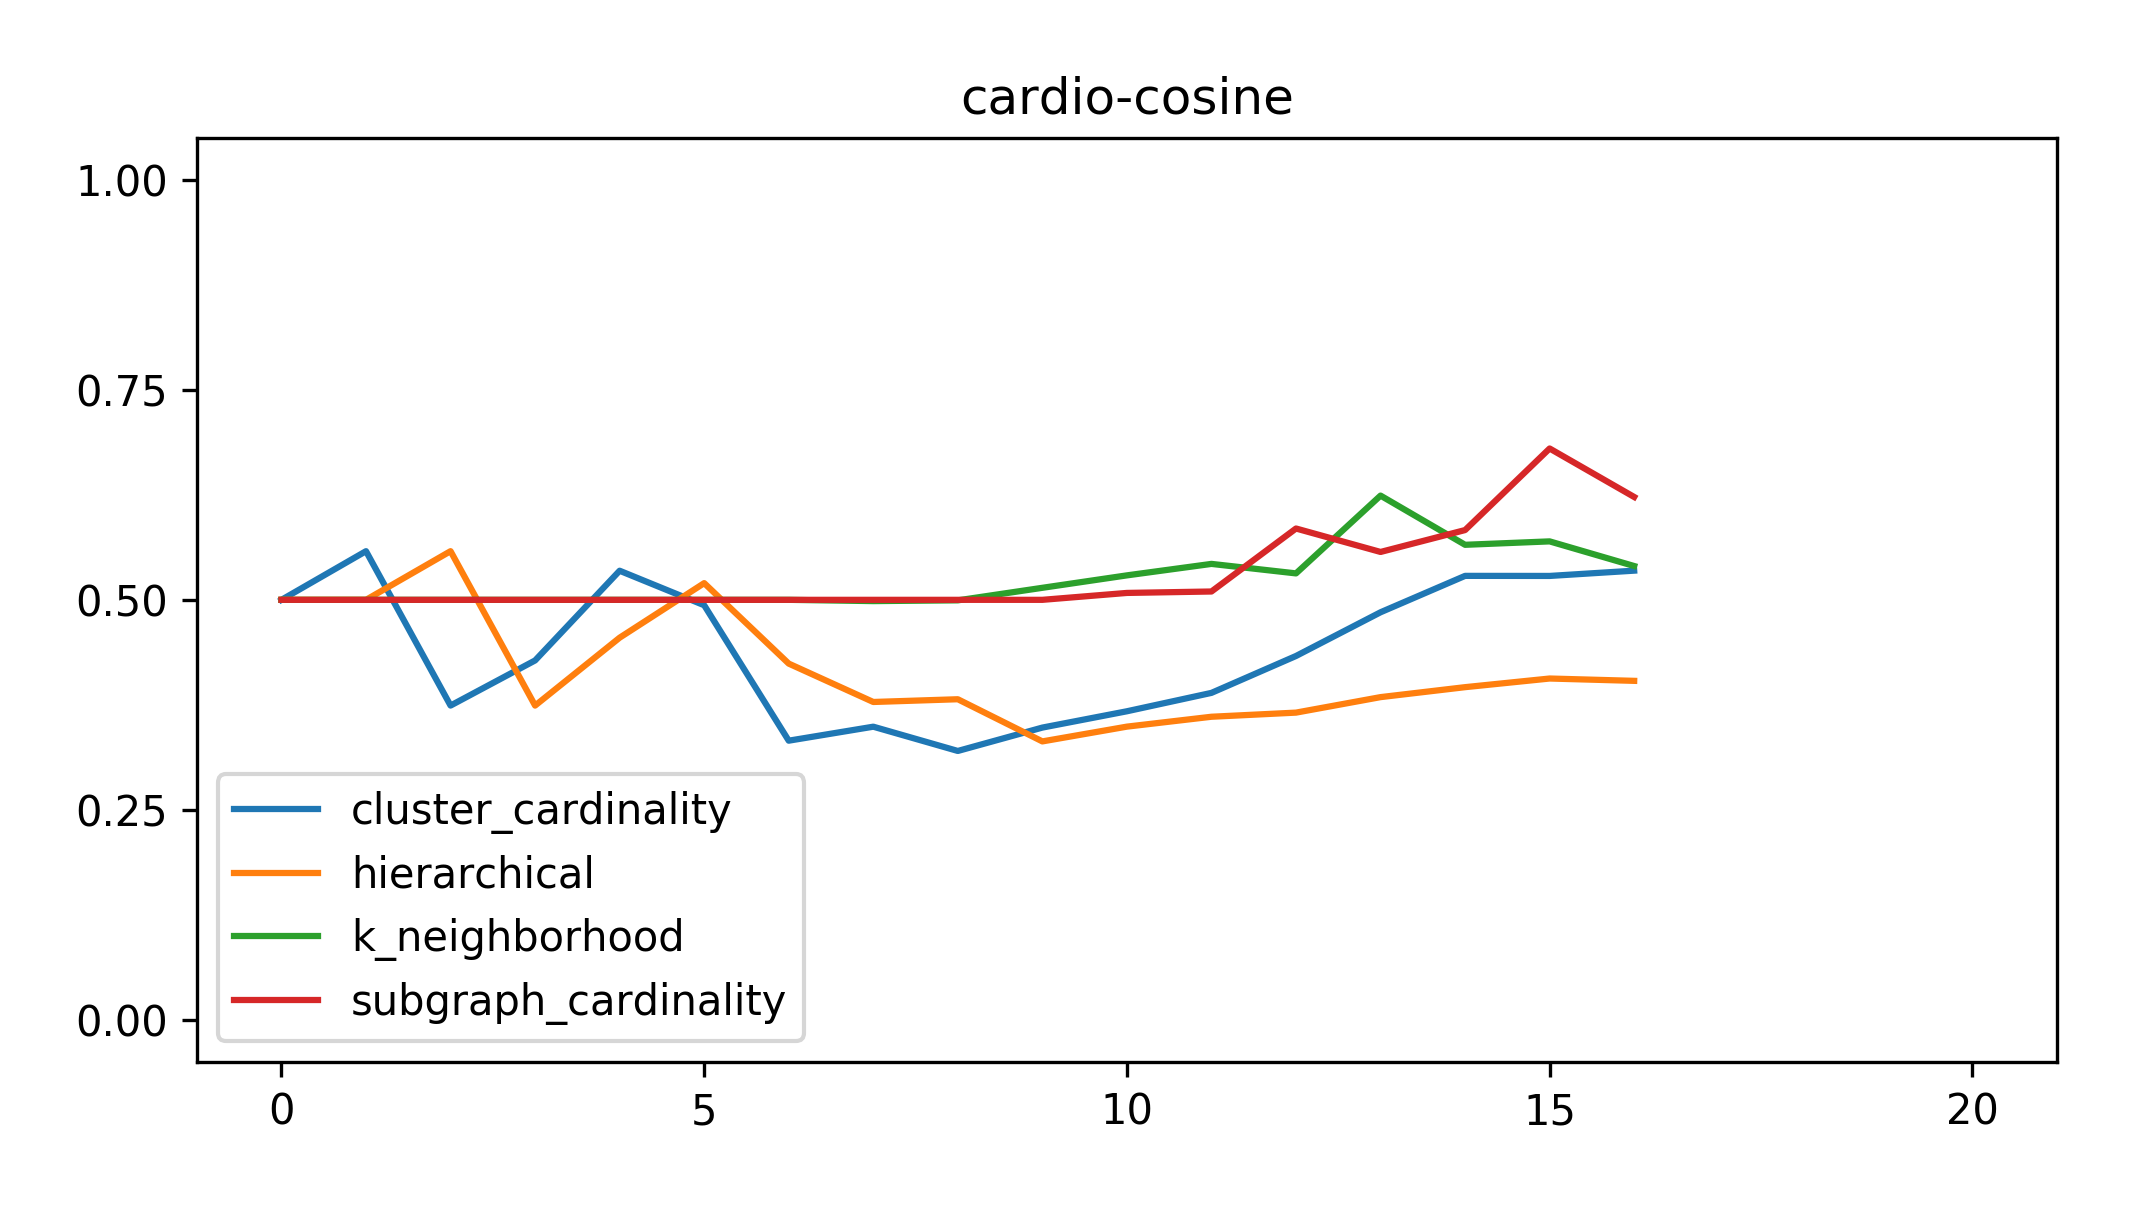
\includegraphics[width=2.2in]{kdd/static/auc_vs_depth/cardio-cosine.png}
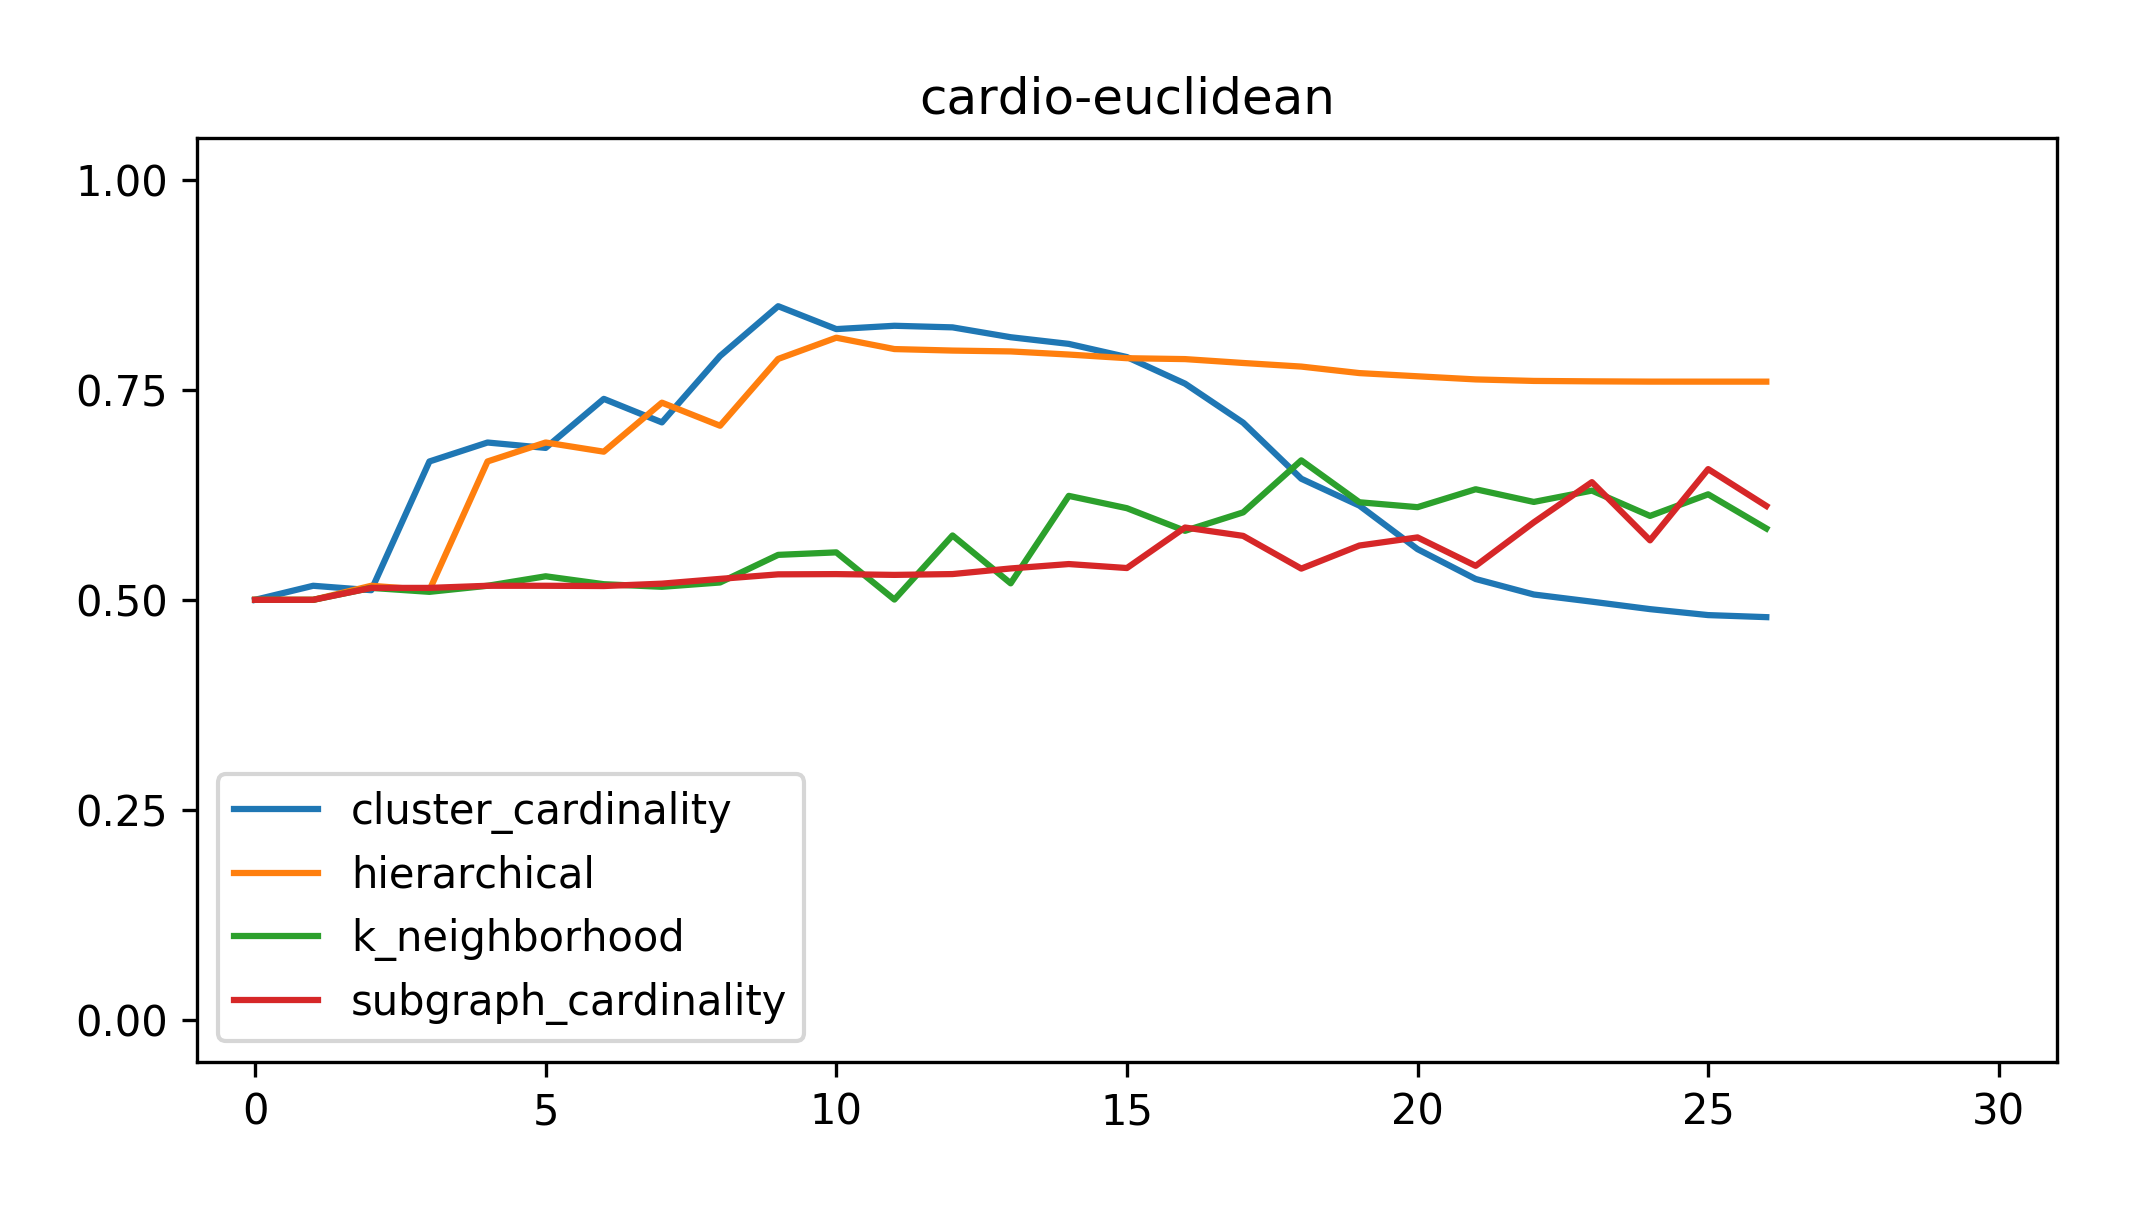
\includegraphics[width=2.2in]{kdd/static/auc_vs_depth/cardio-euclidean.png}
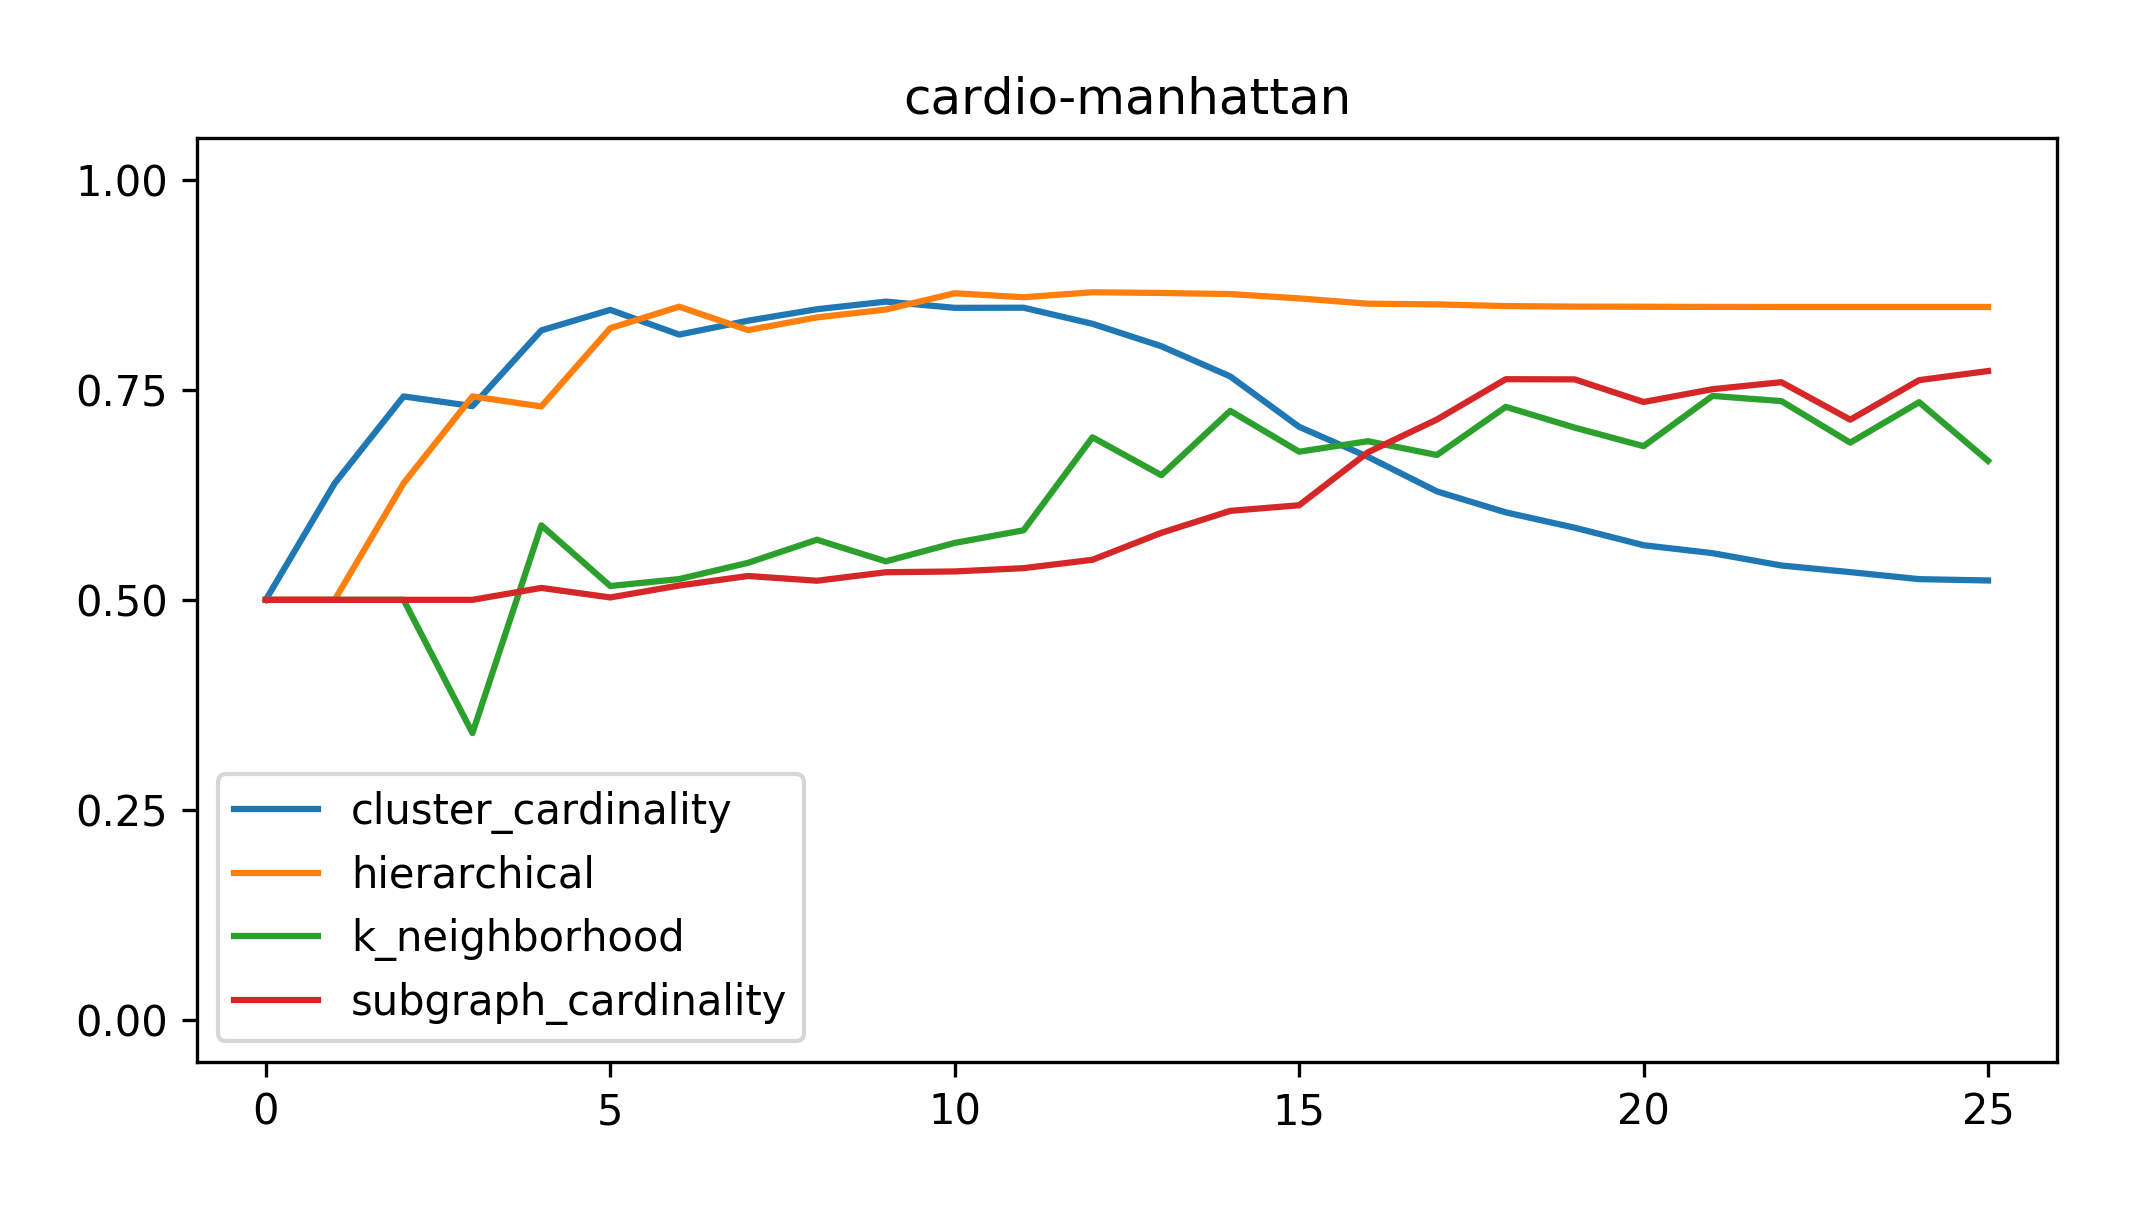
\includegraphics[width=2.2in]{kdd/static/auc_vs_depth/cardio-manhattan.png}

% Glass
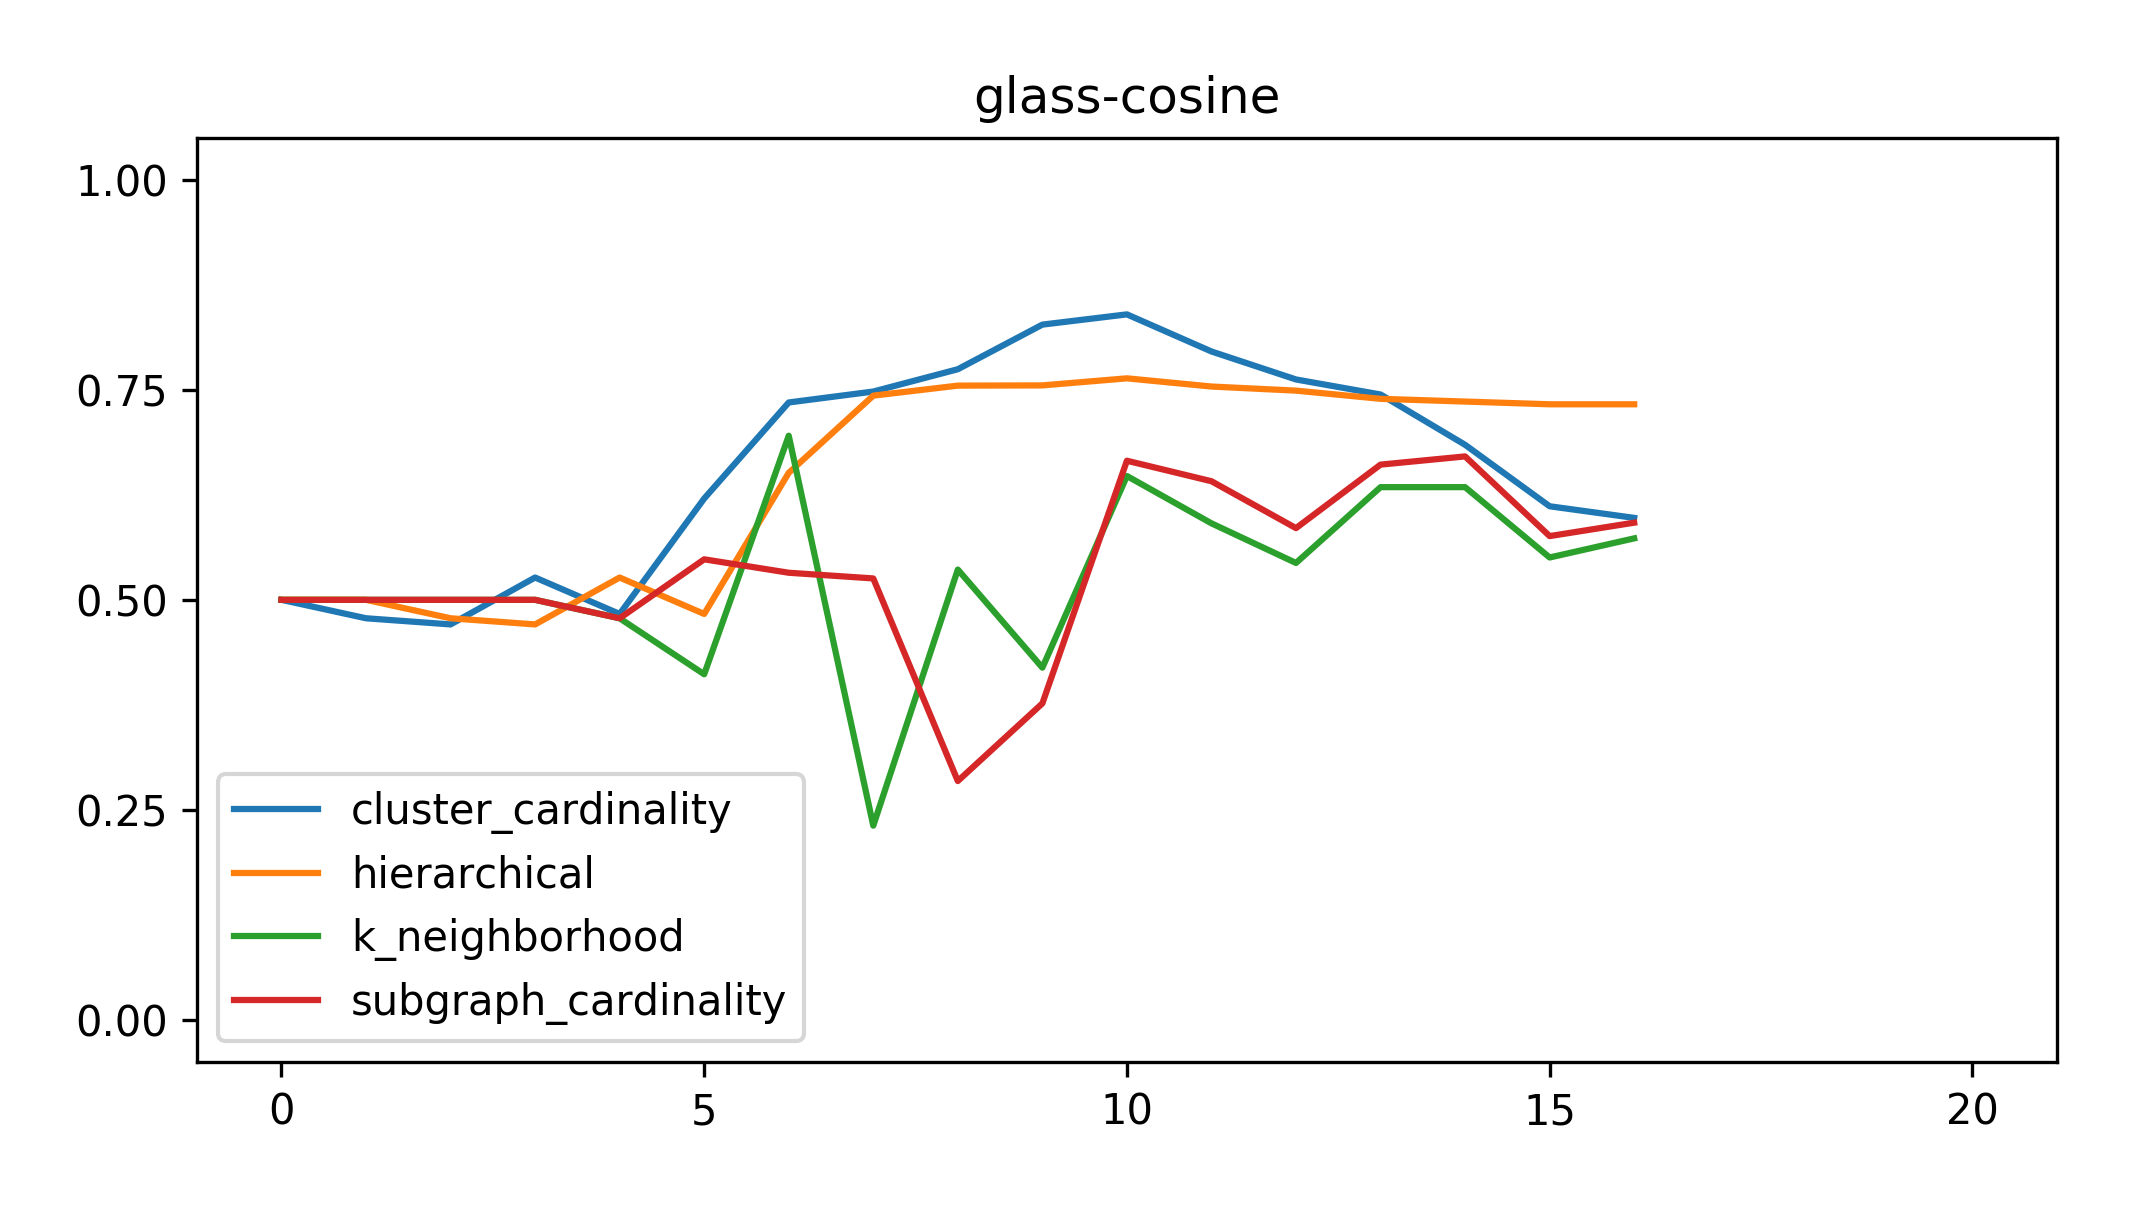
\includegraphics[width=2.2in]{kdd/static/auc_vs_depth/glass-cosine.png}
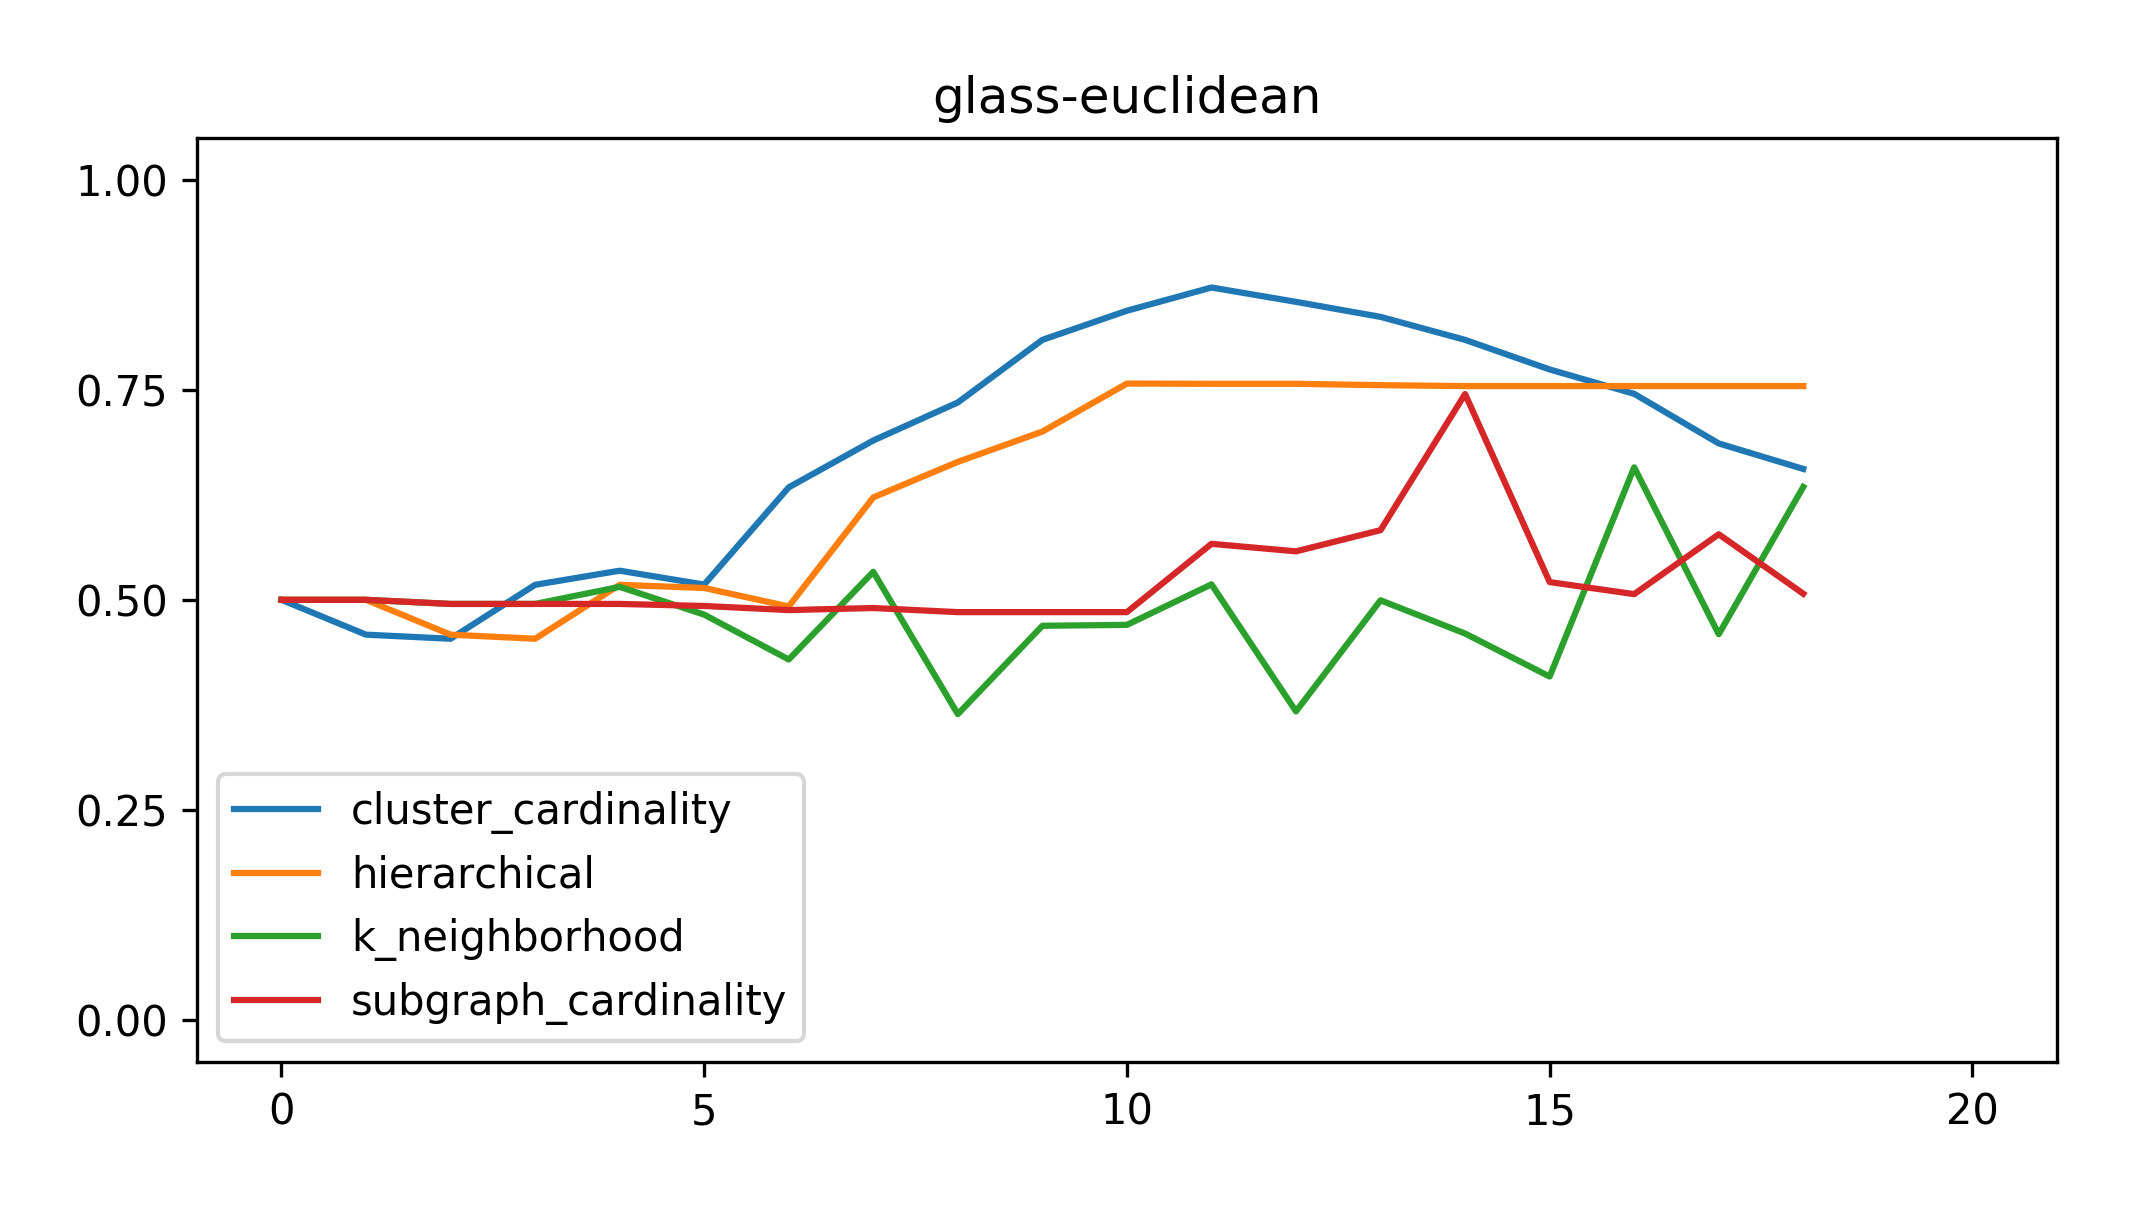
\includegraphics[width=2.2in]{kdd/static/auc_vs_depth/glass-euclidean.png}
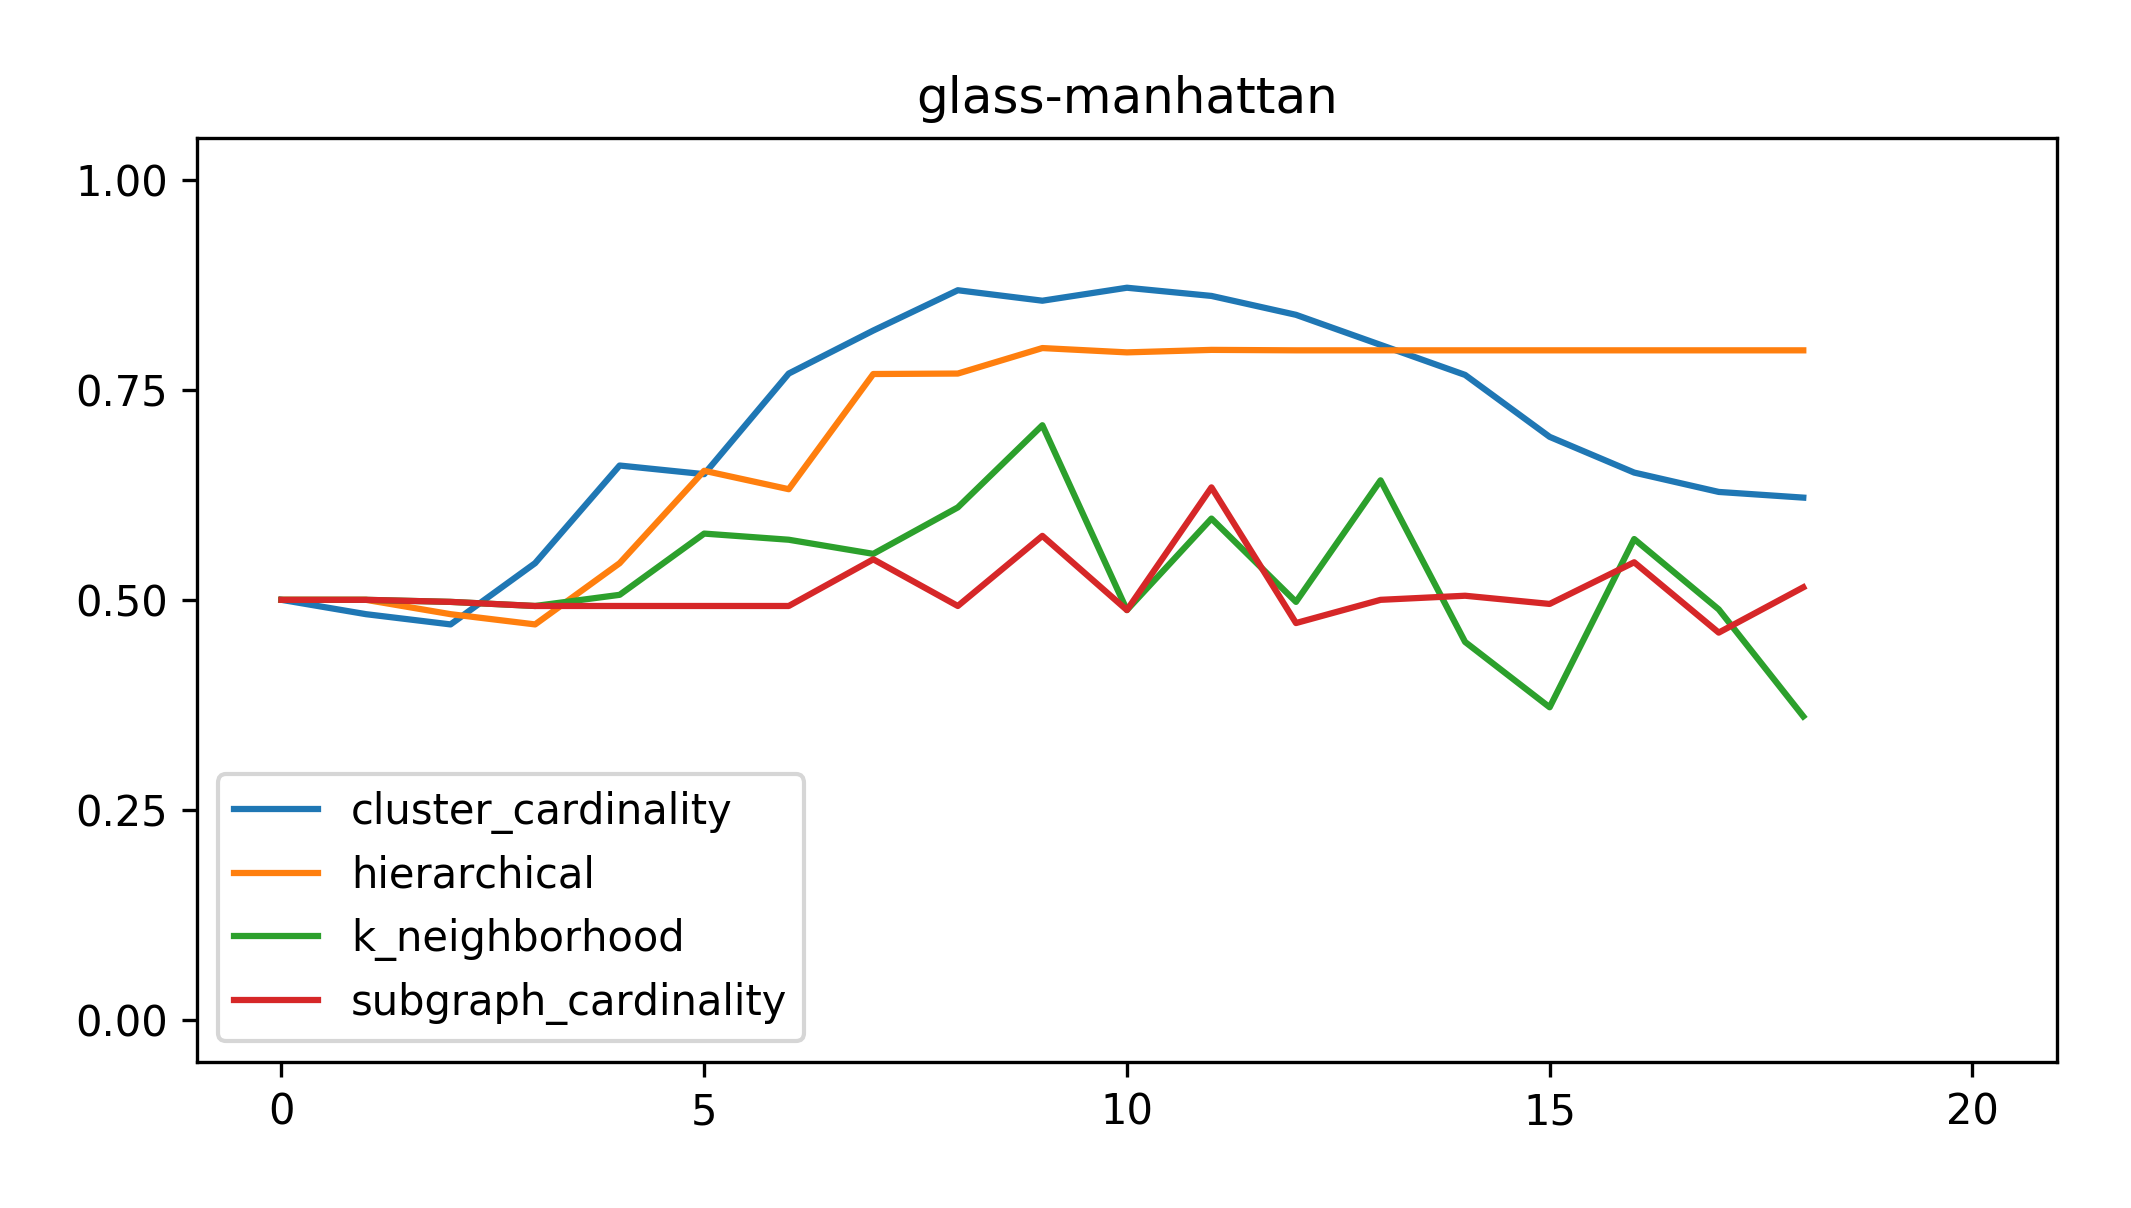
\includegraphics[width=2.2in]{kdd/static/auc_vs_depth/glass-manhattan.png}

% Ionosphere
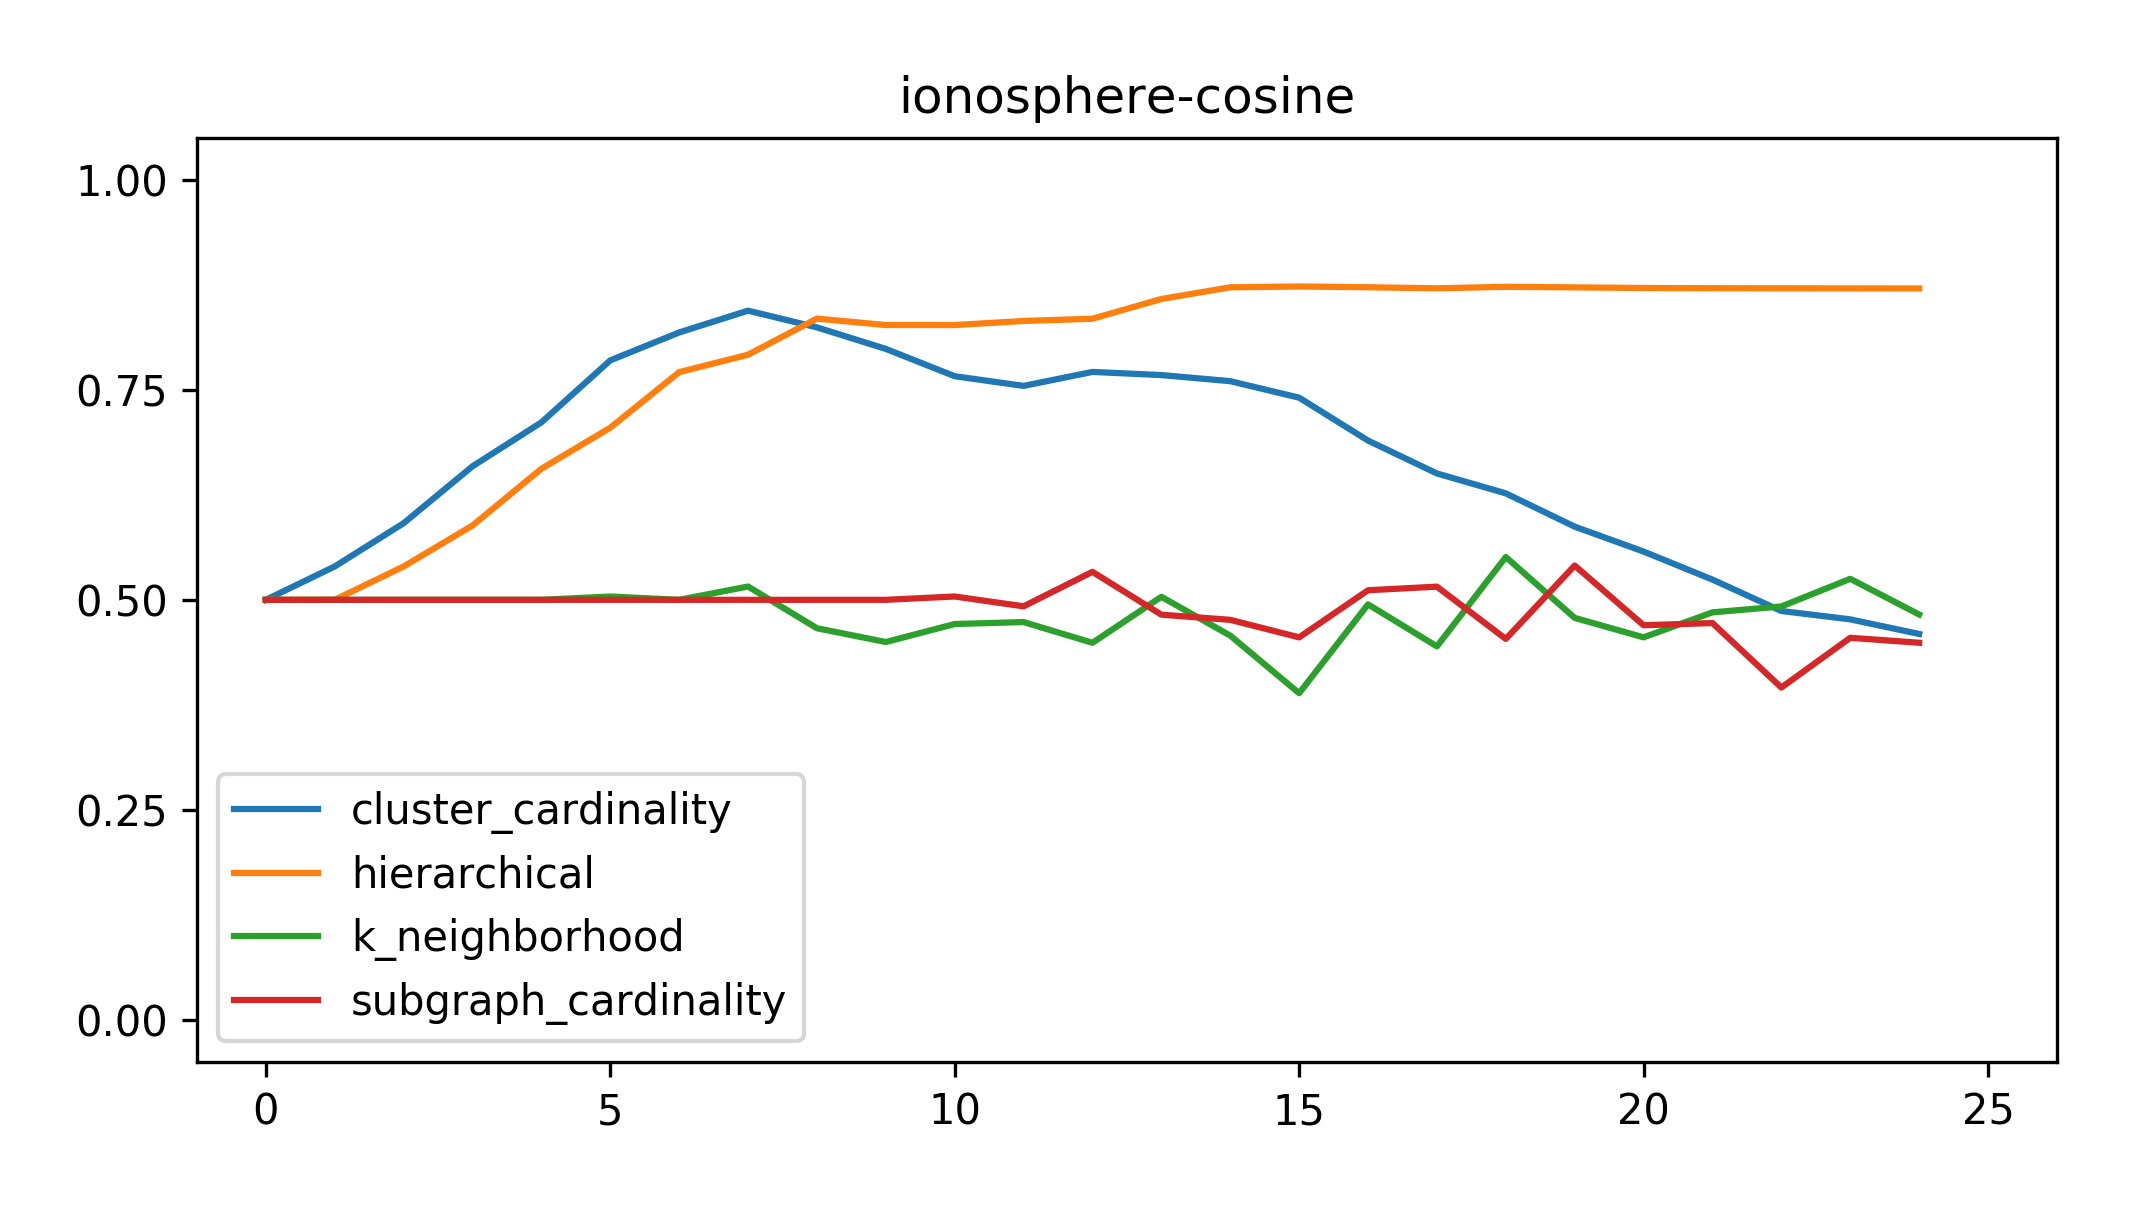
\includegraphics[width=2.2in]{kdd/static/auc_vs_depth/ionosphere-cosine.png}
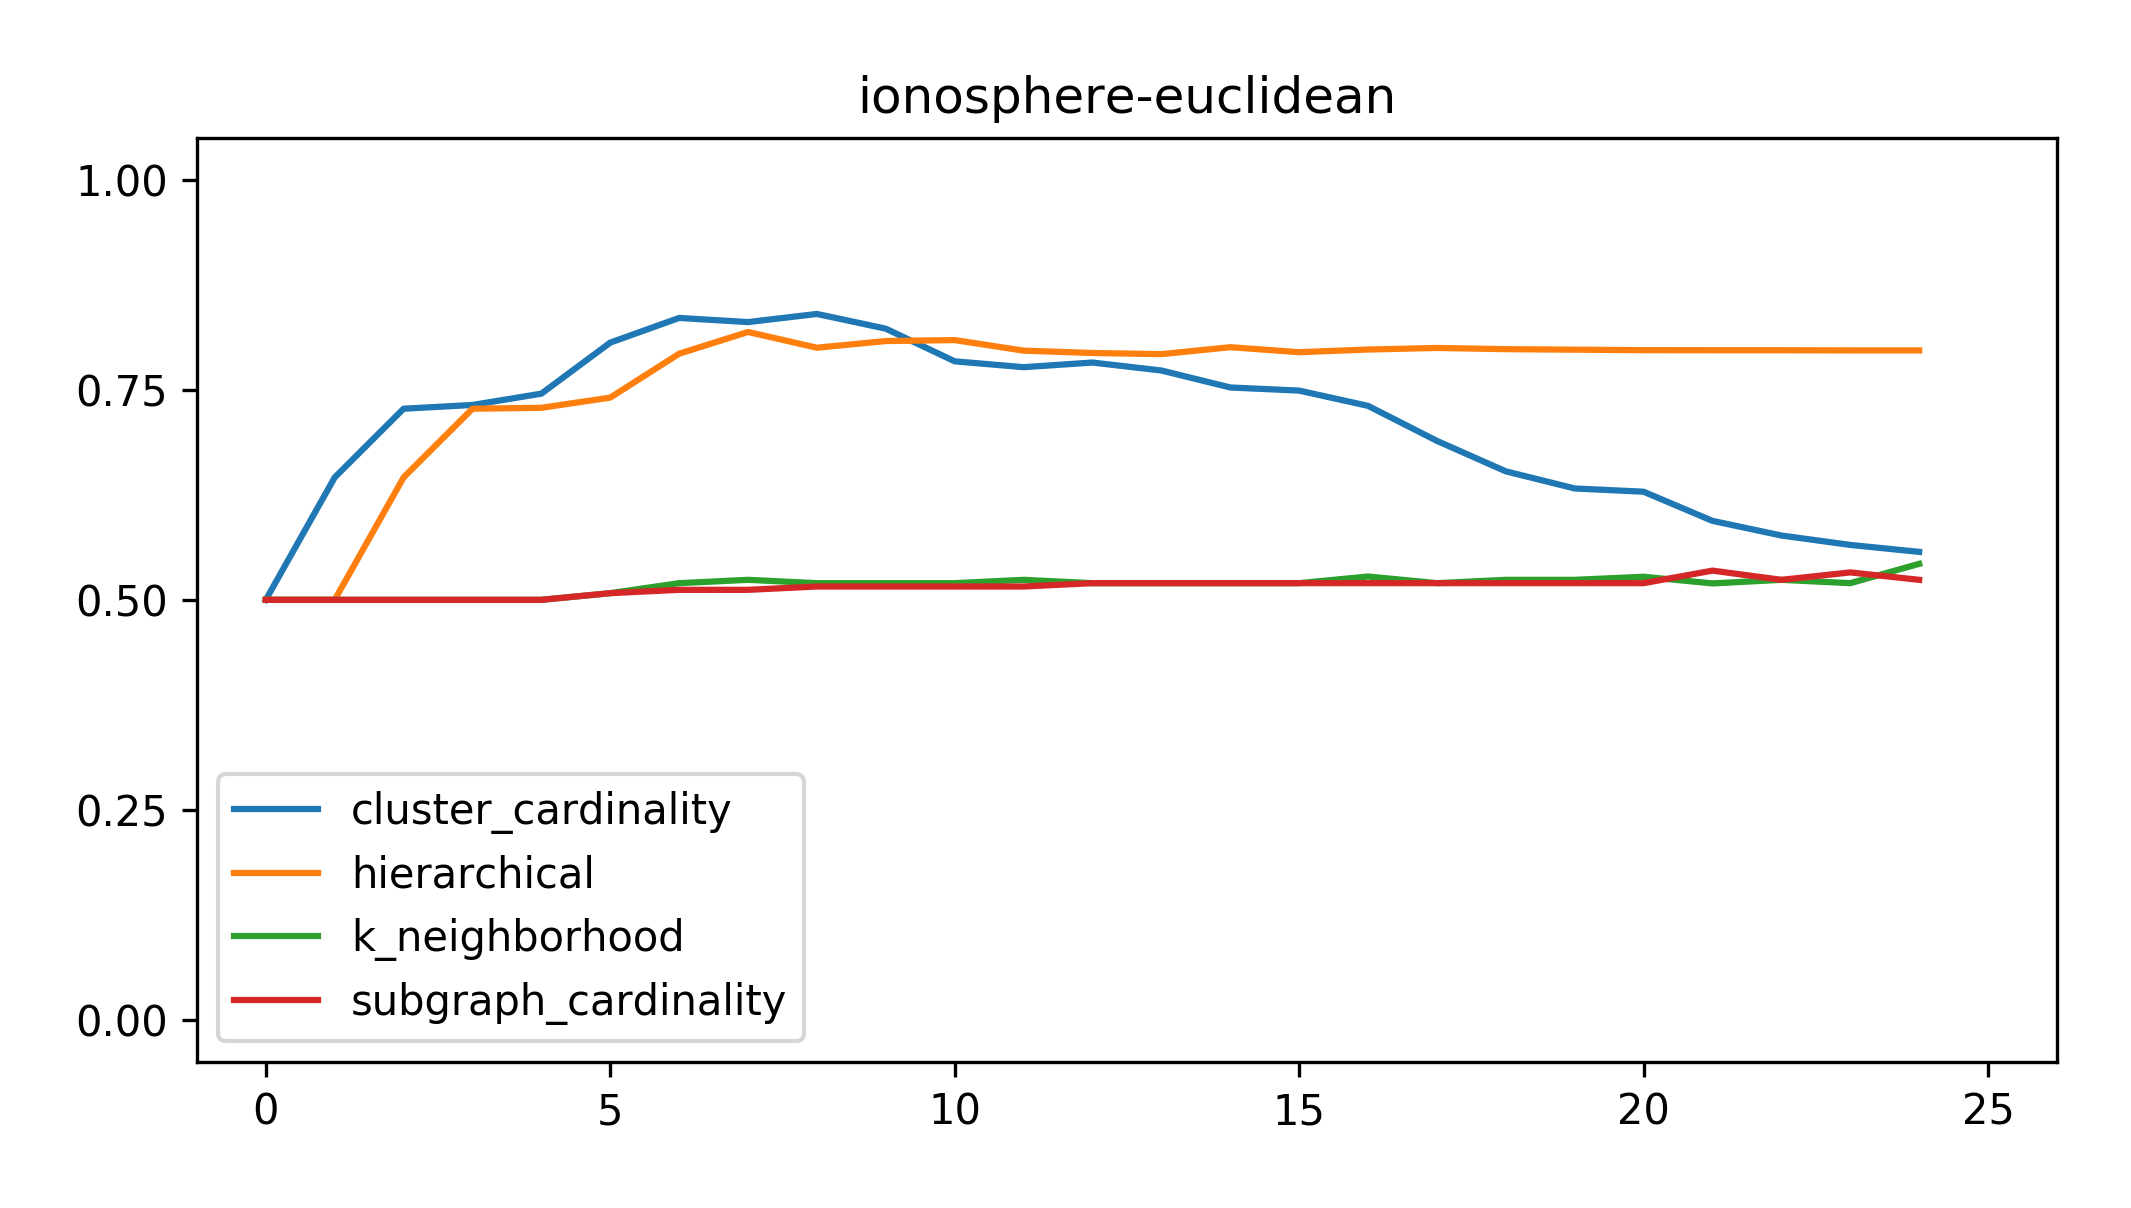
\includegraphics[width=2.2in]{kdd/static/auc_vs_depth/ionosphere-euclidean.png}
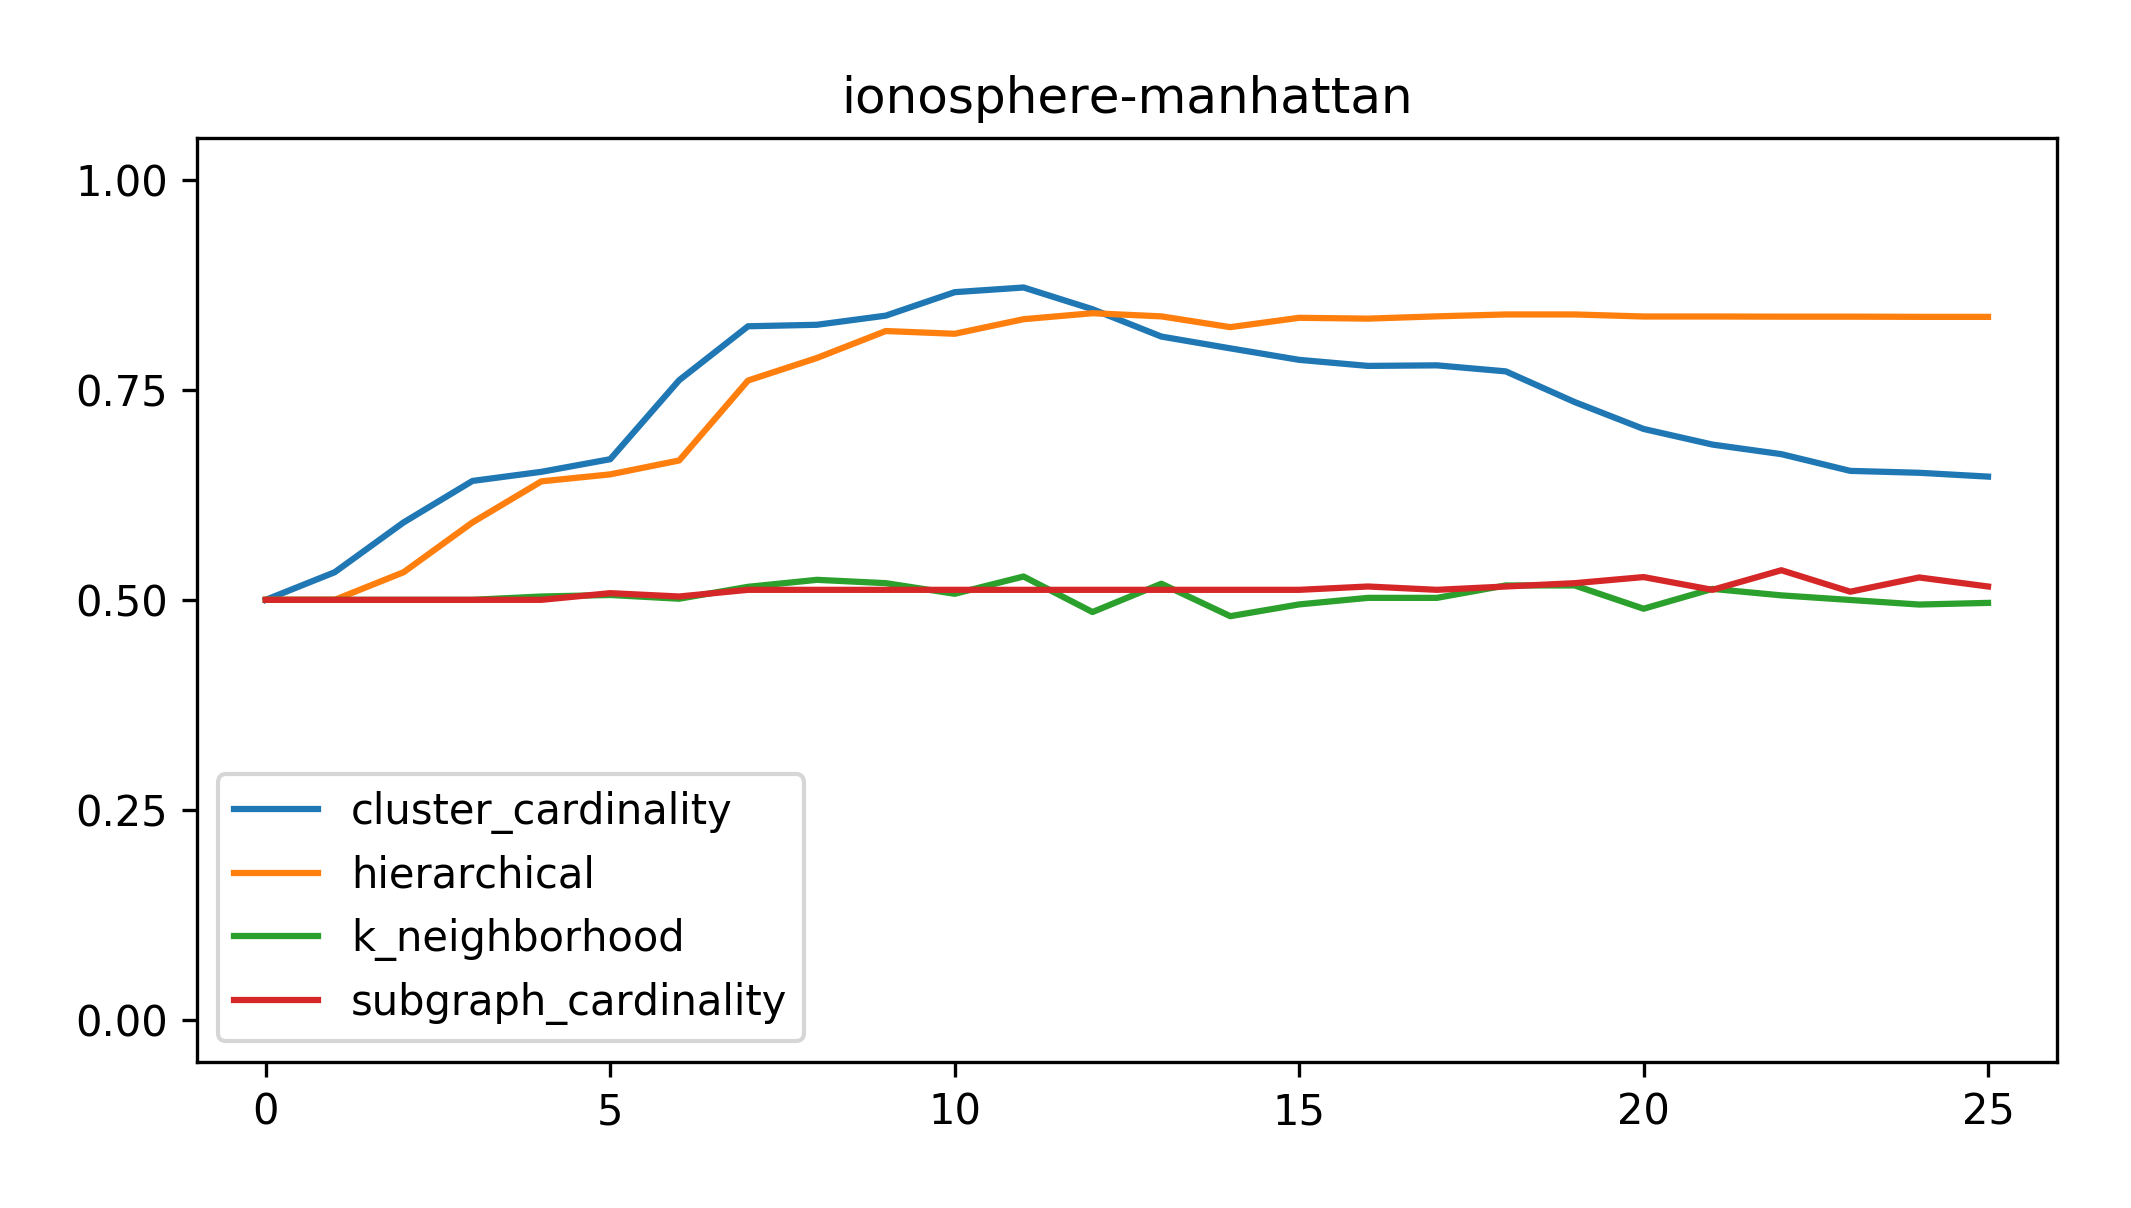
\includegraphics[width=2.2in]{kdd/static/auc_vs_depth/ionosphere-manhattan.png}

\caption{
Plots of ROC-AUC vs Depth for our mearures of Anomolousness.
}

\label{results:datasets_1}
\end{figure*}

\begin{figure*}[!t]
\centering
% Lympho
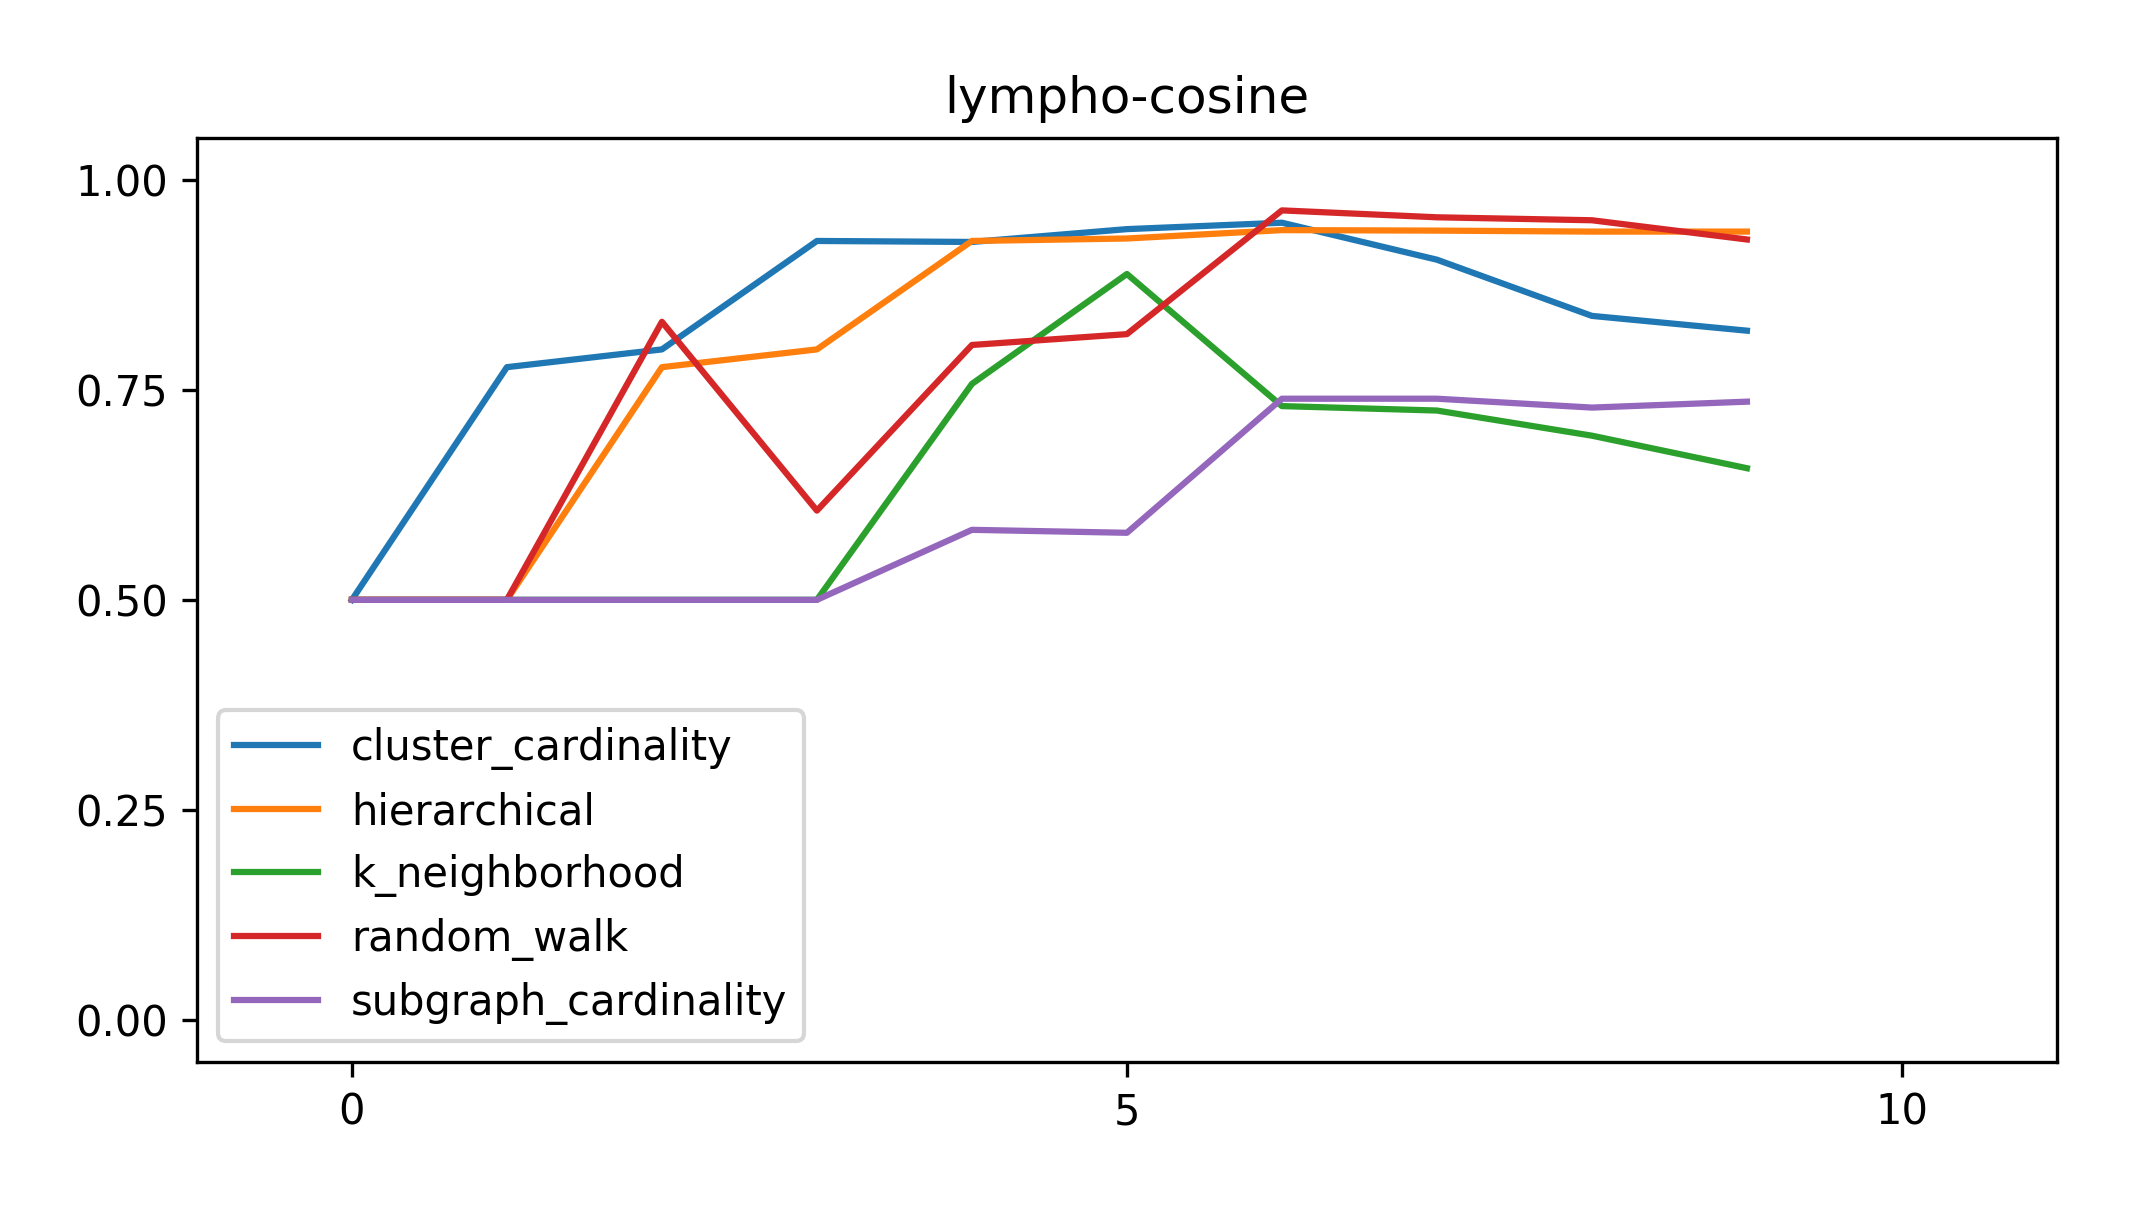
\includegraphics[width=2.2in]{kdd/static/auc_vs_depth/lympho-cosine.png}
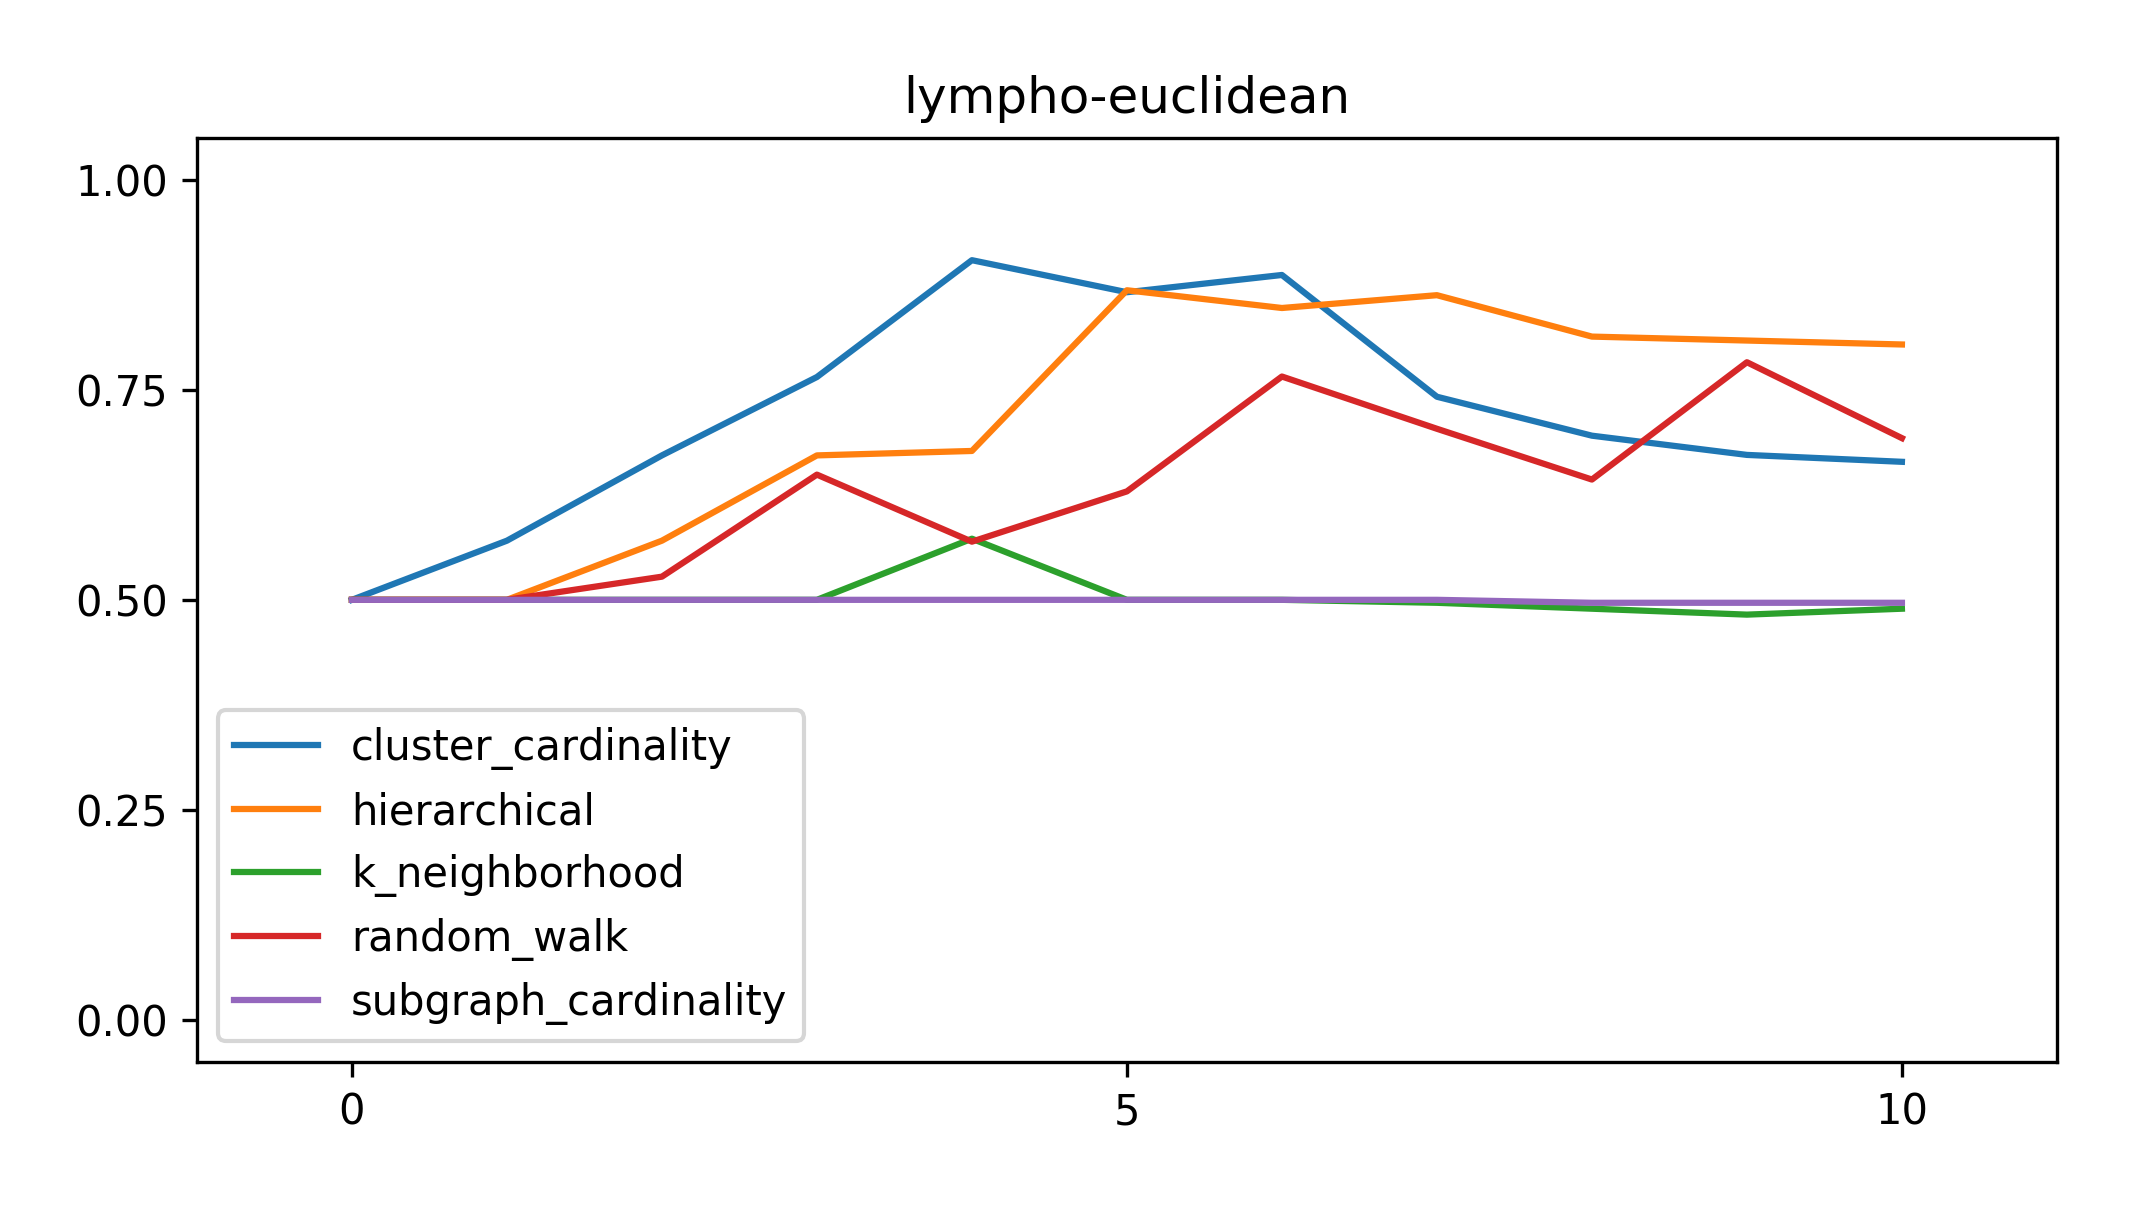
\includegraphics[width=2.2in]{kdd/static/auc_vs_depth/lympho-euclidean.png}
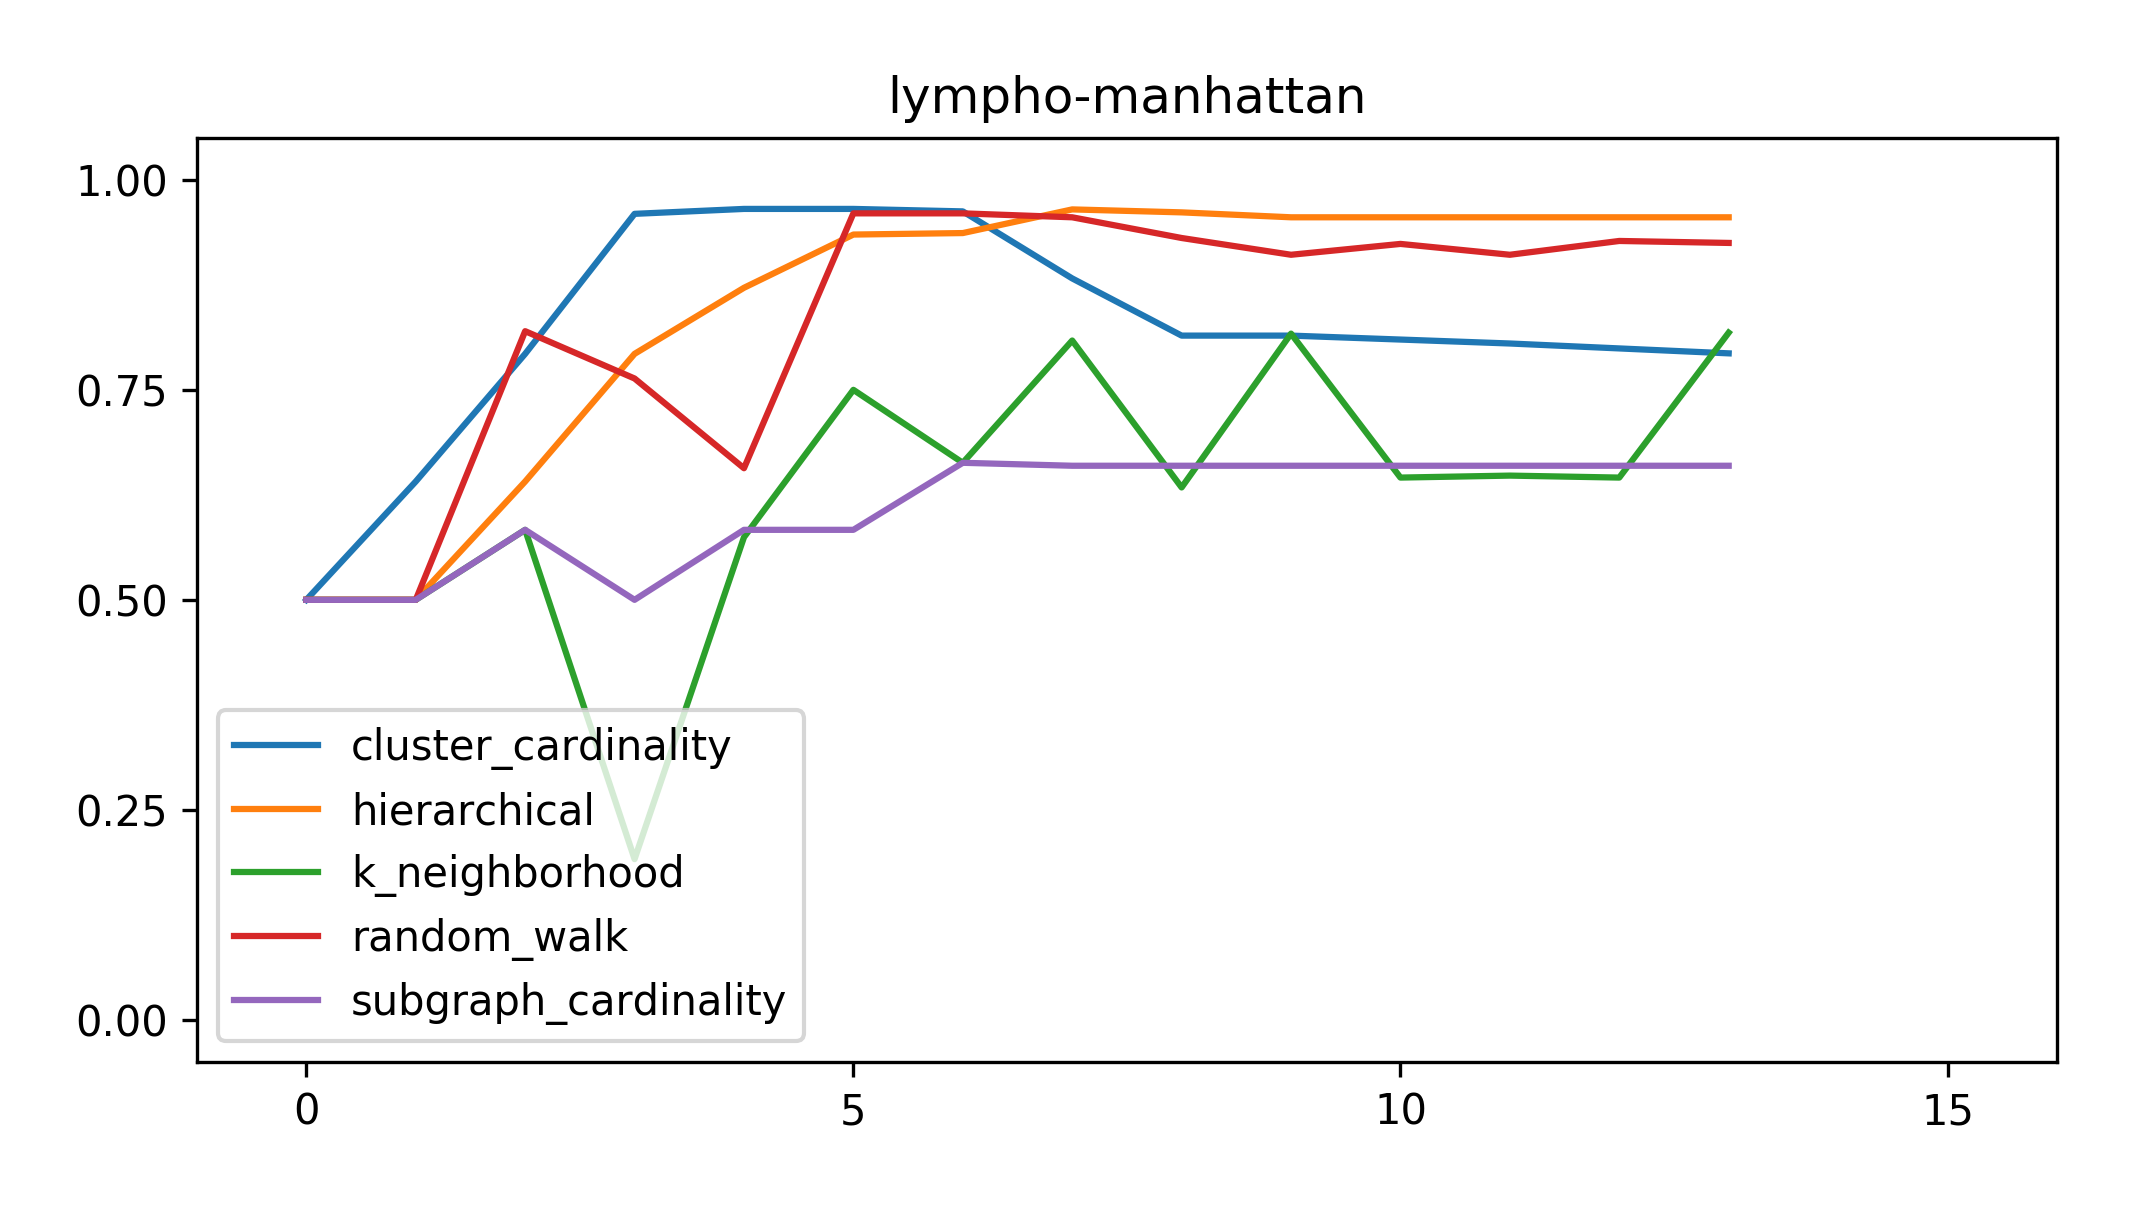
\includegraphics[width=2.2in]{kdd/static/auc_vs_depth/lympho-manhattan.png}

% Mnist
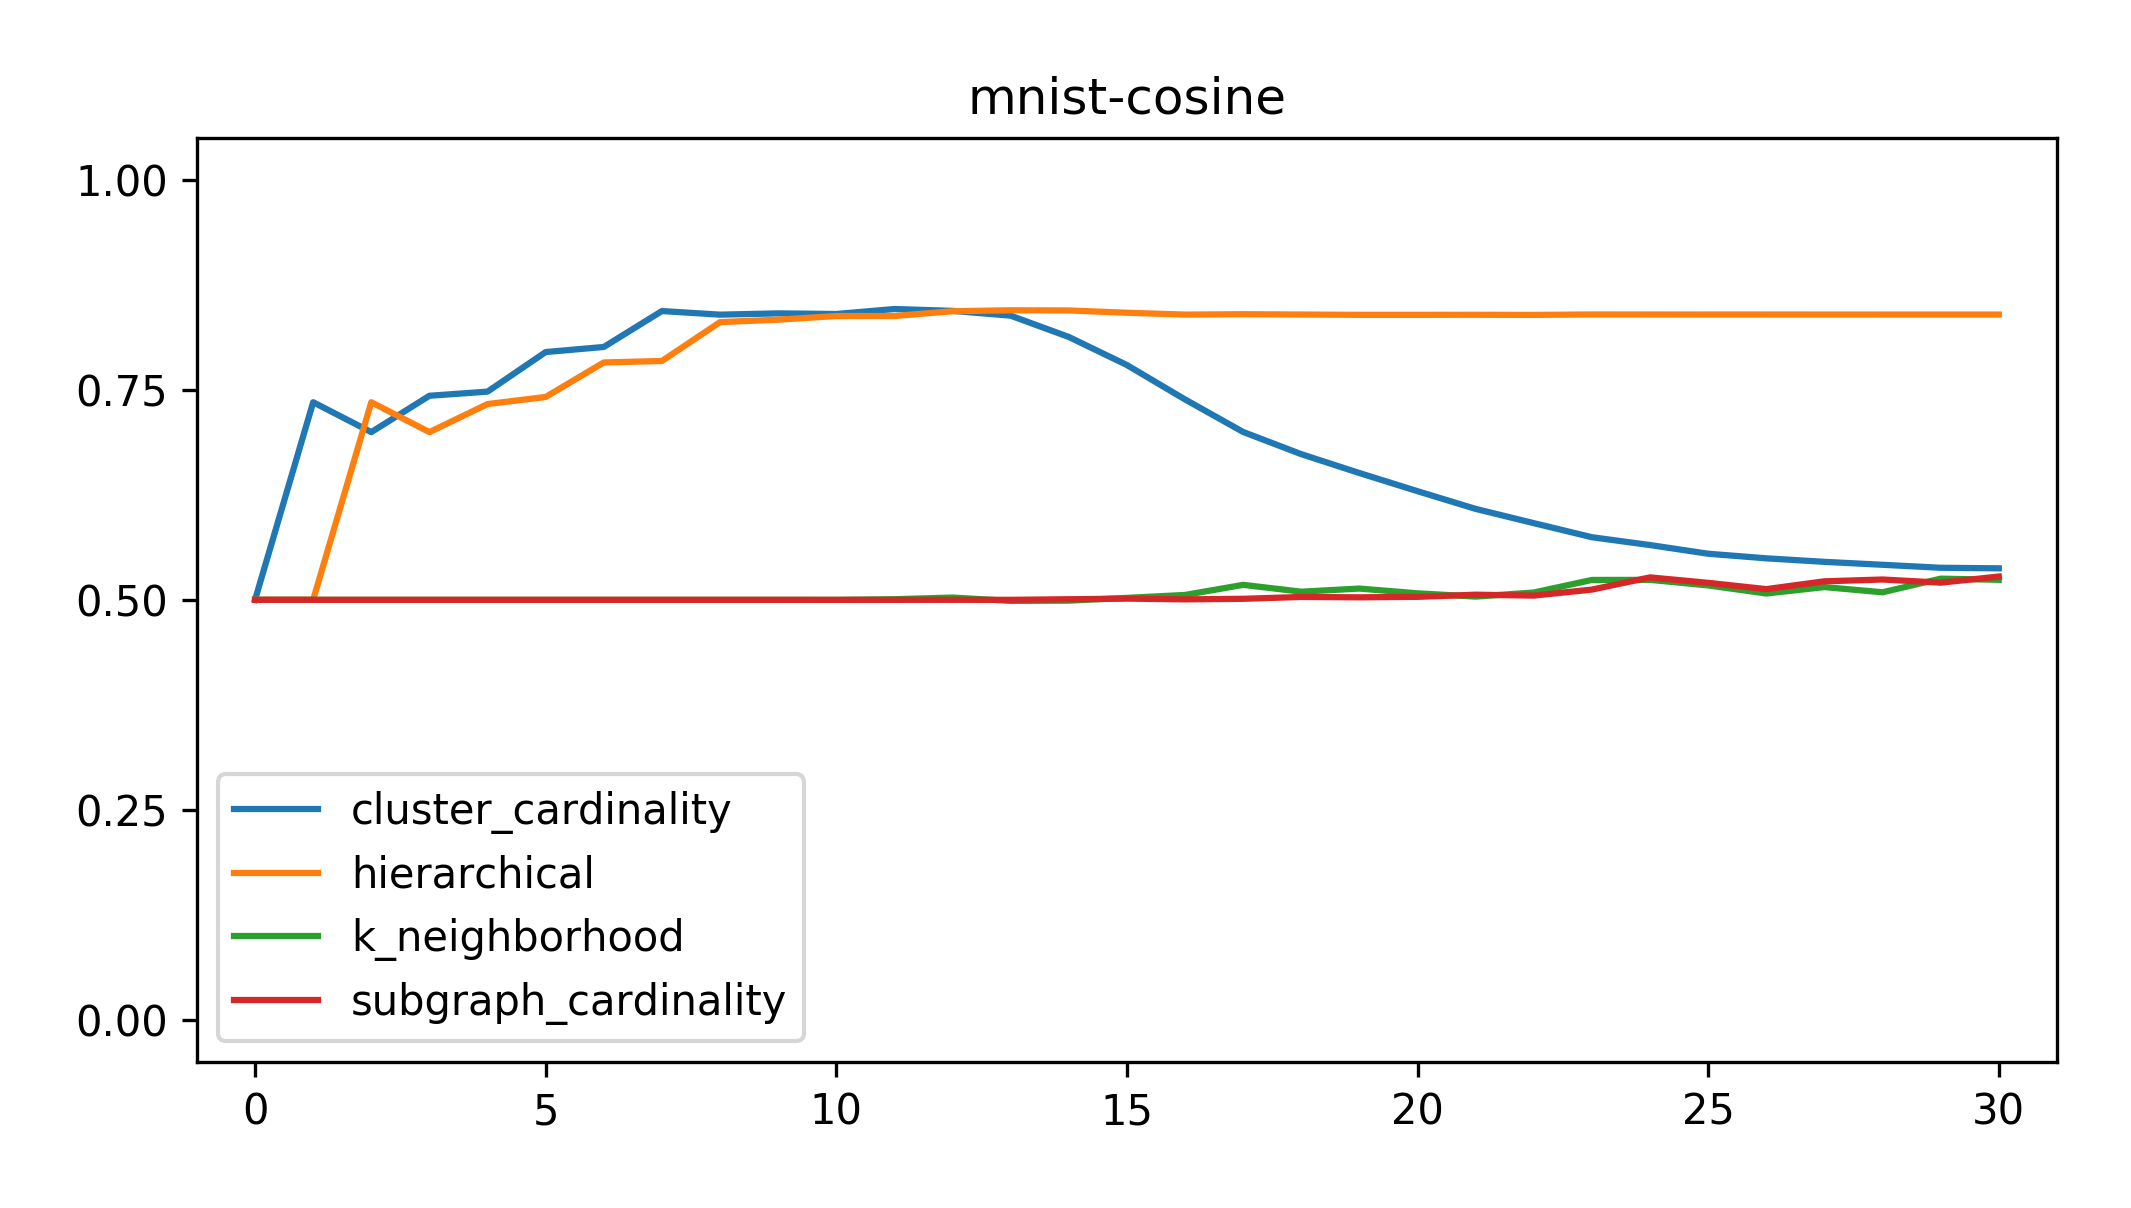
\includegraphics[width=2.2in]{kdd/static/auc_vs_depth/mnist-cosine.png}
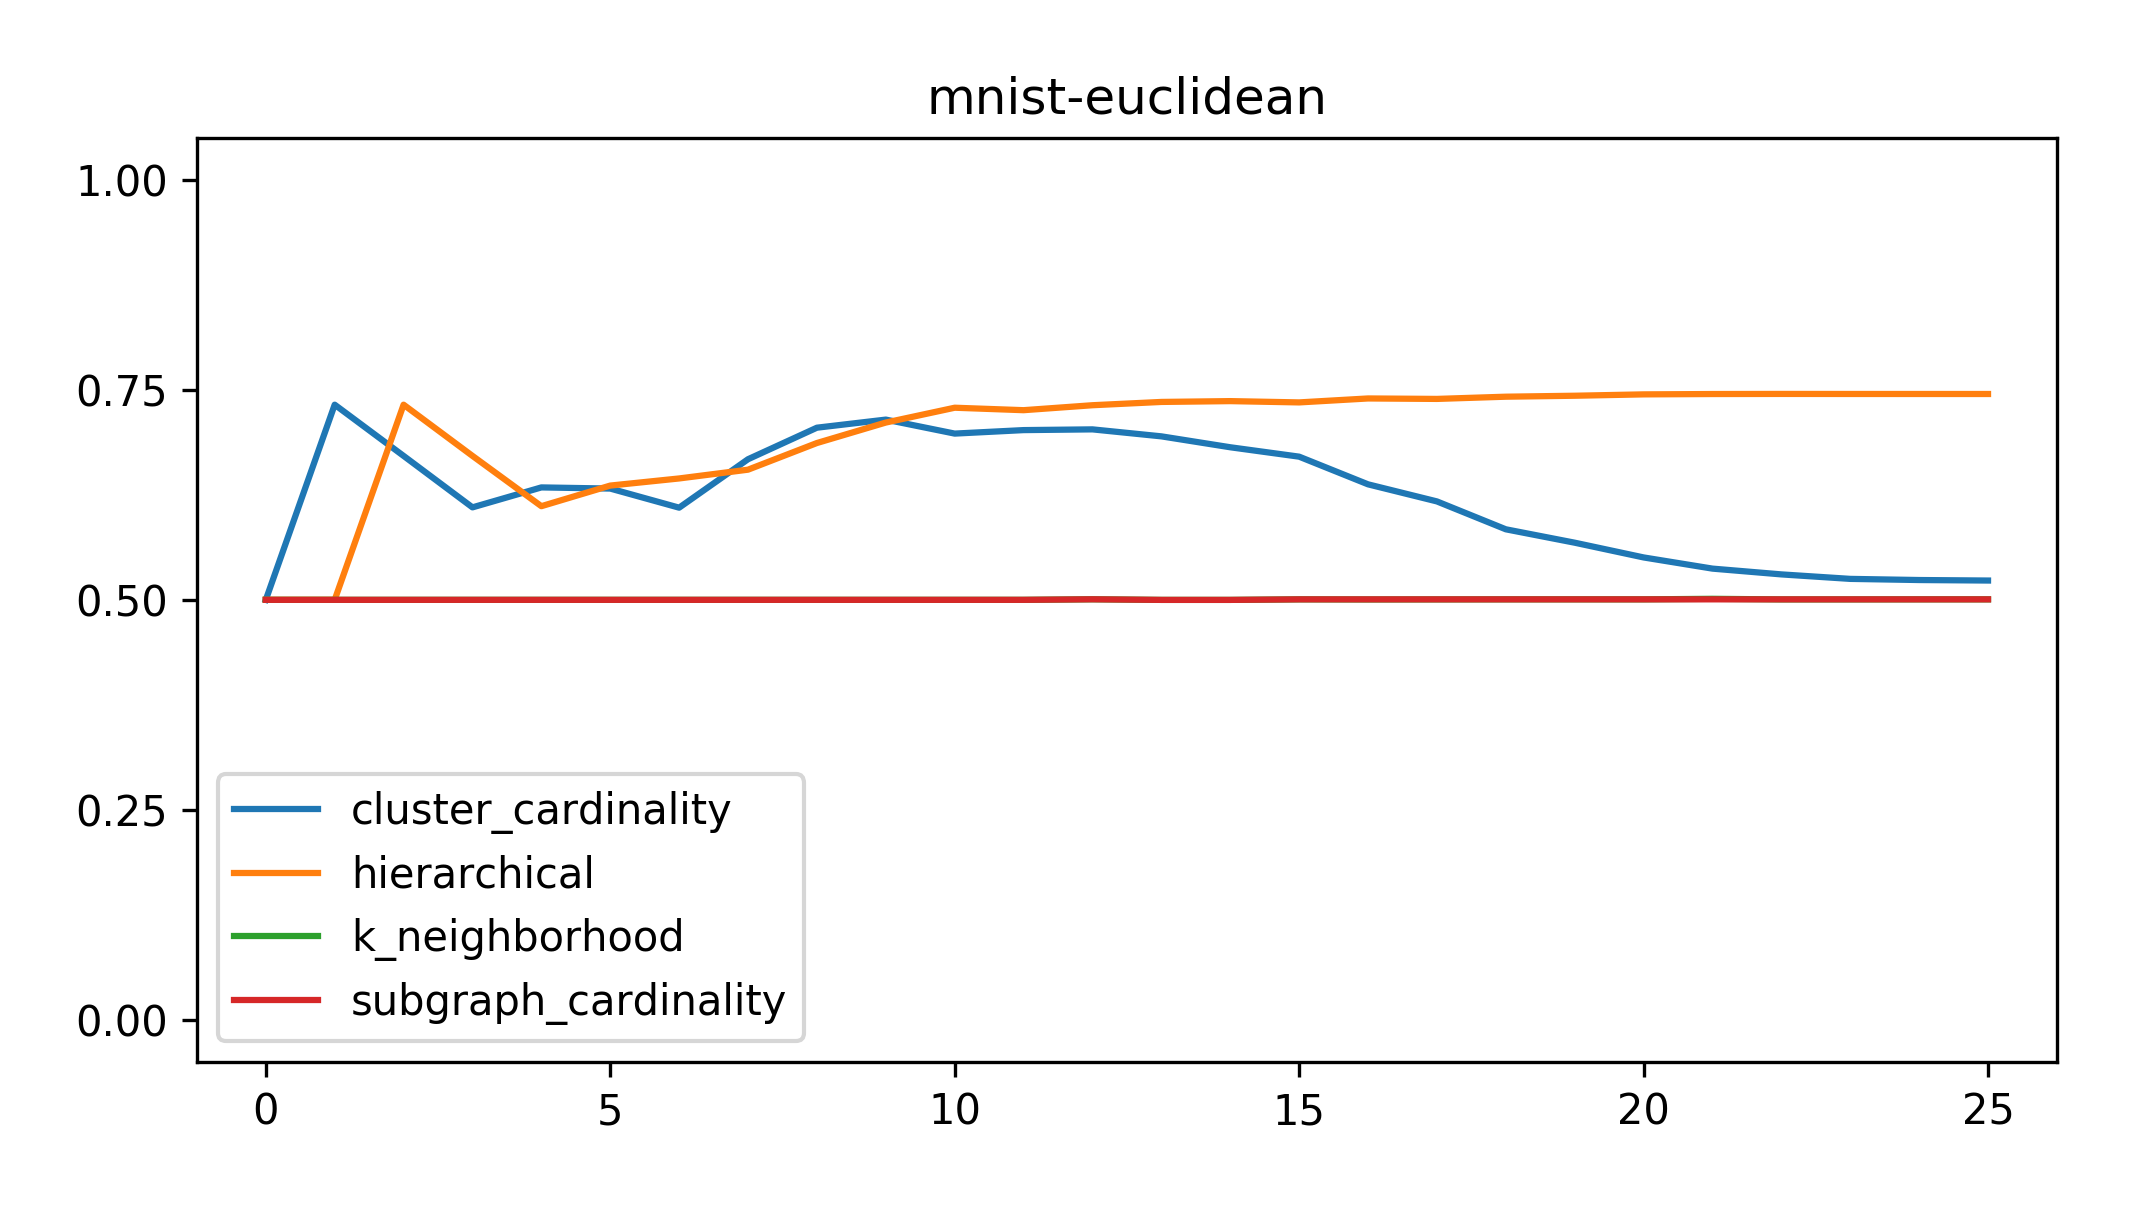
\includegraphics[width=2.2in]{kdd/static/auc_vs_depth/mnist-euclidean.png}
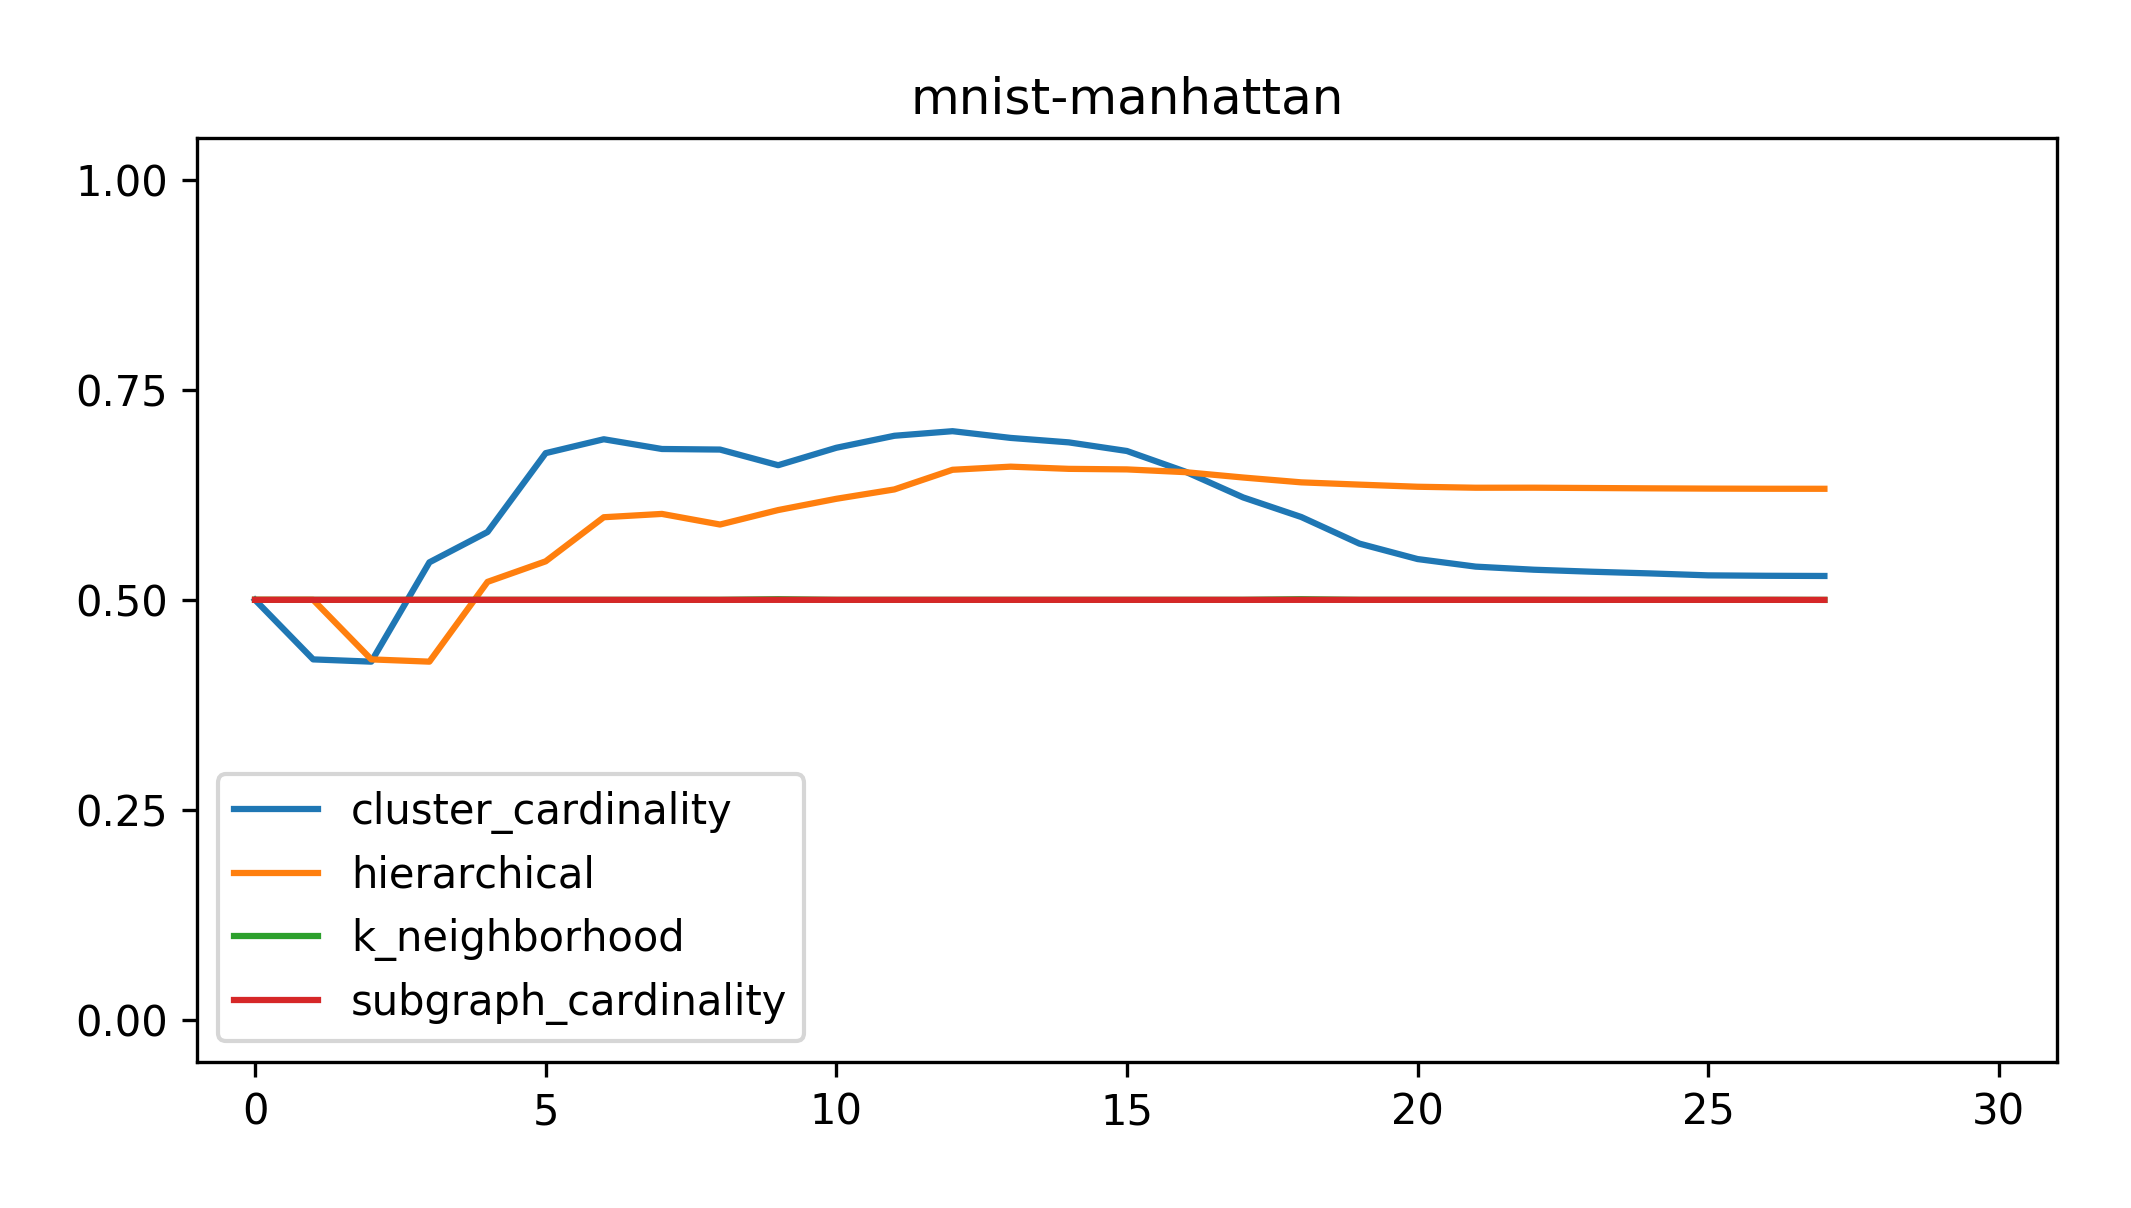
\includegraphics[width=2.2in]{kdd/static/auc_vs_depth/mnist-manhattan.png}

% Musk
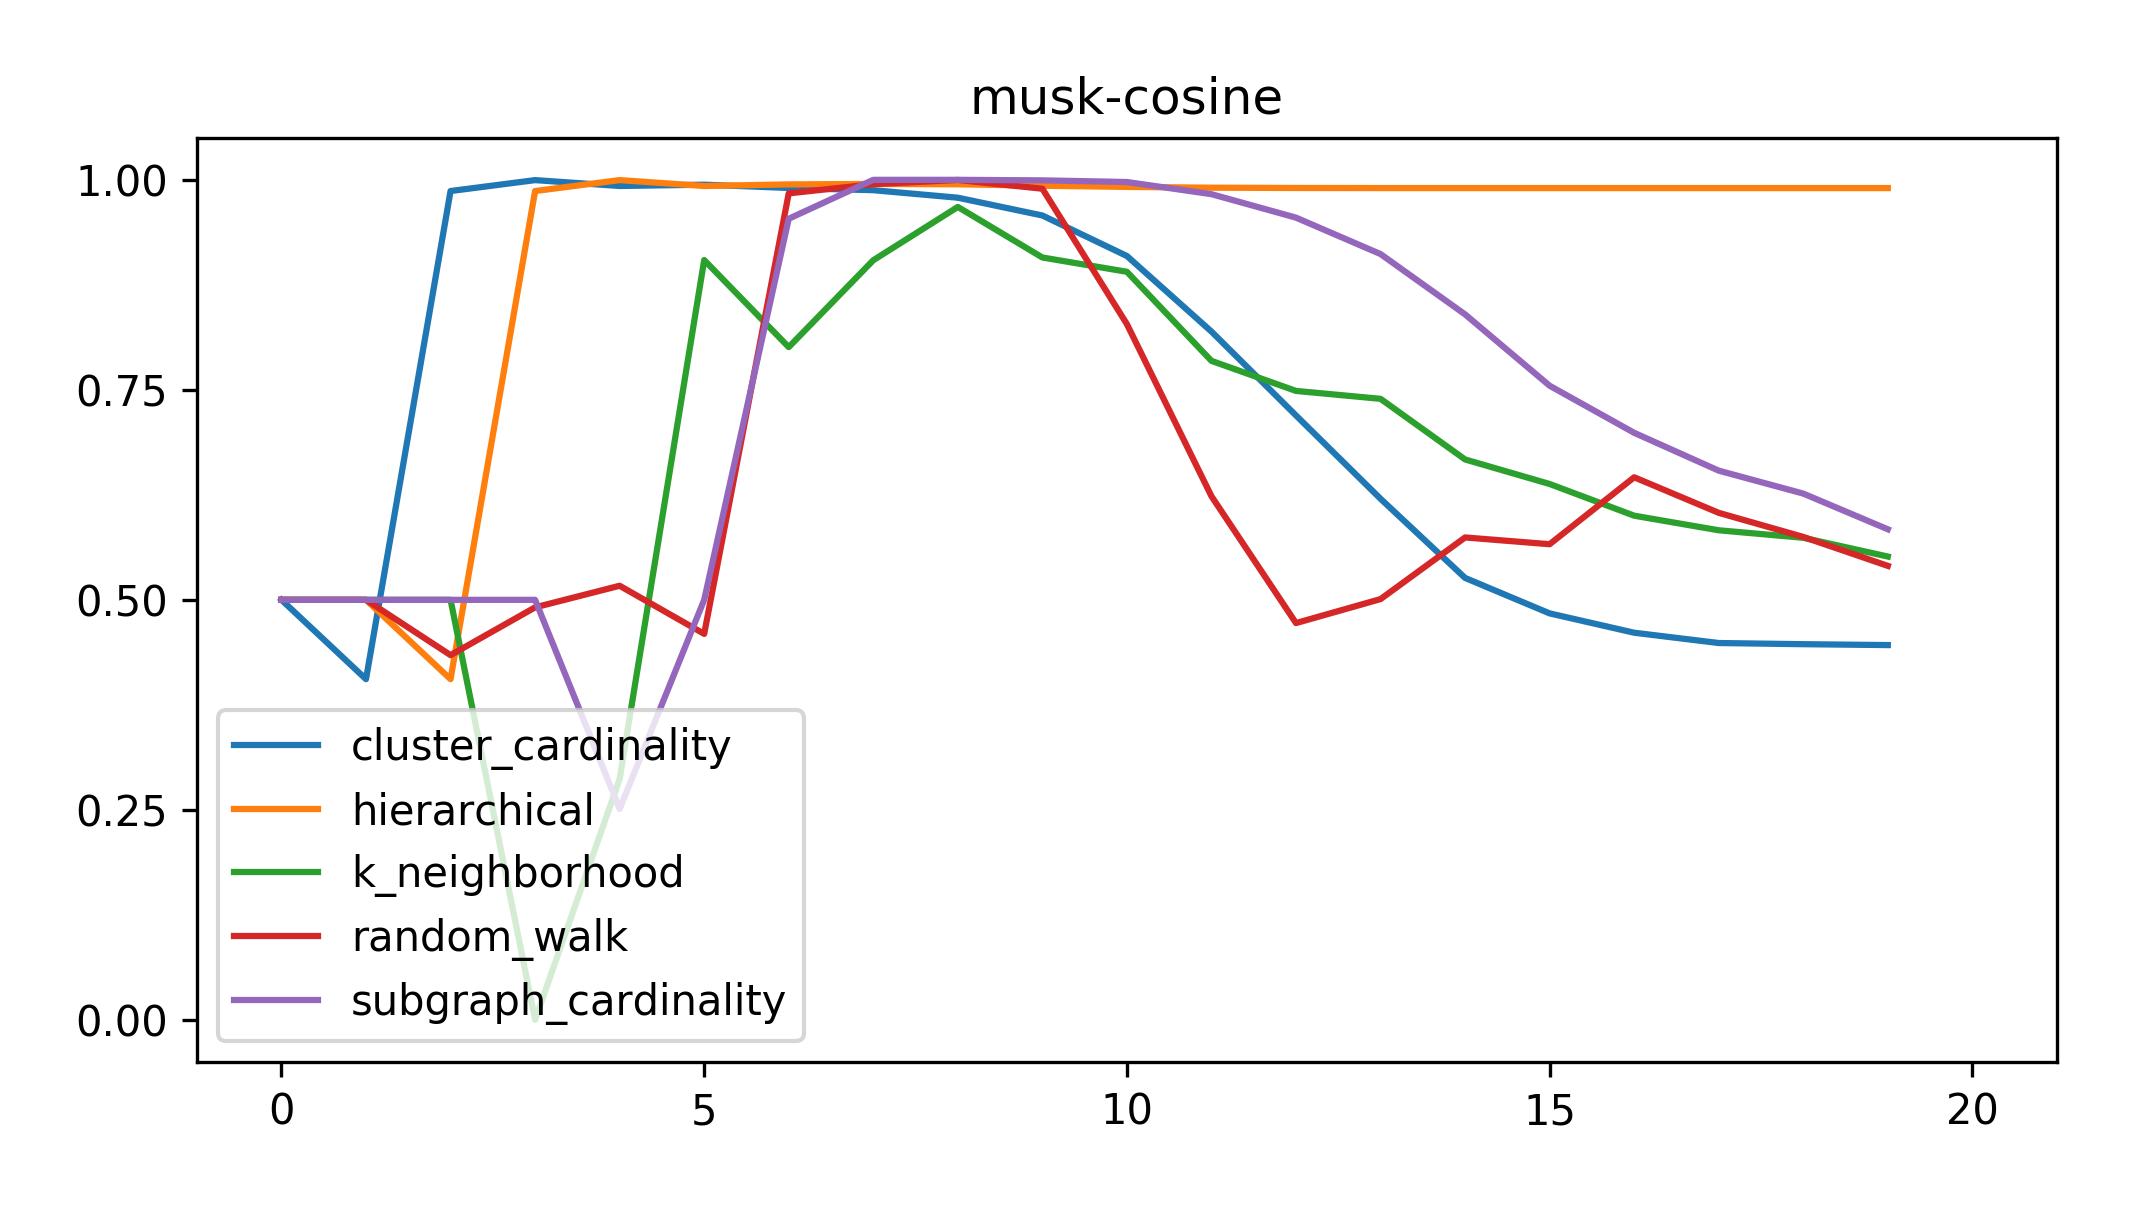
\includegraphics[width=2.2in]{kdd/static/auc_vs_depth/musk-cosine.png}
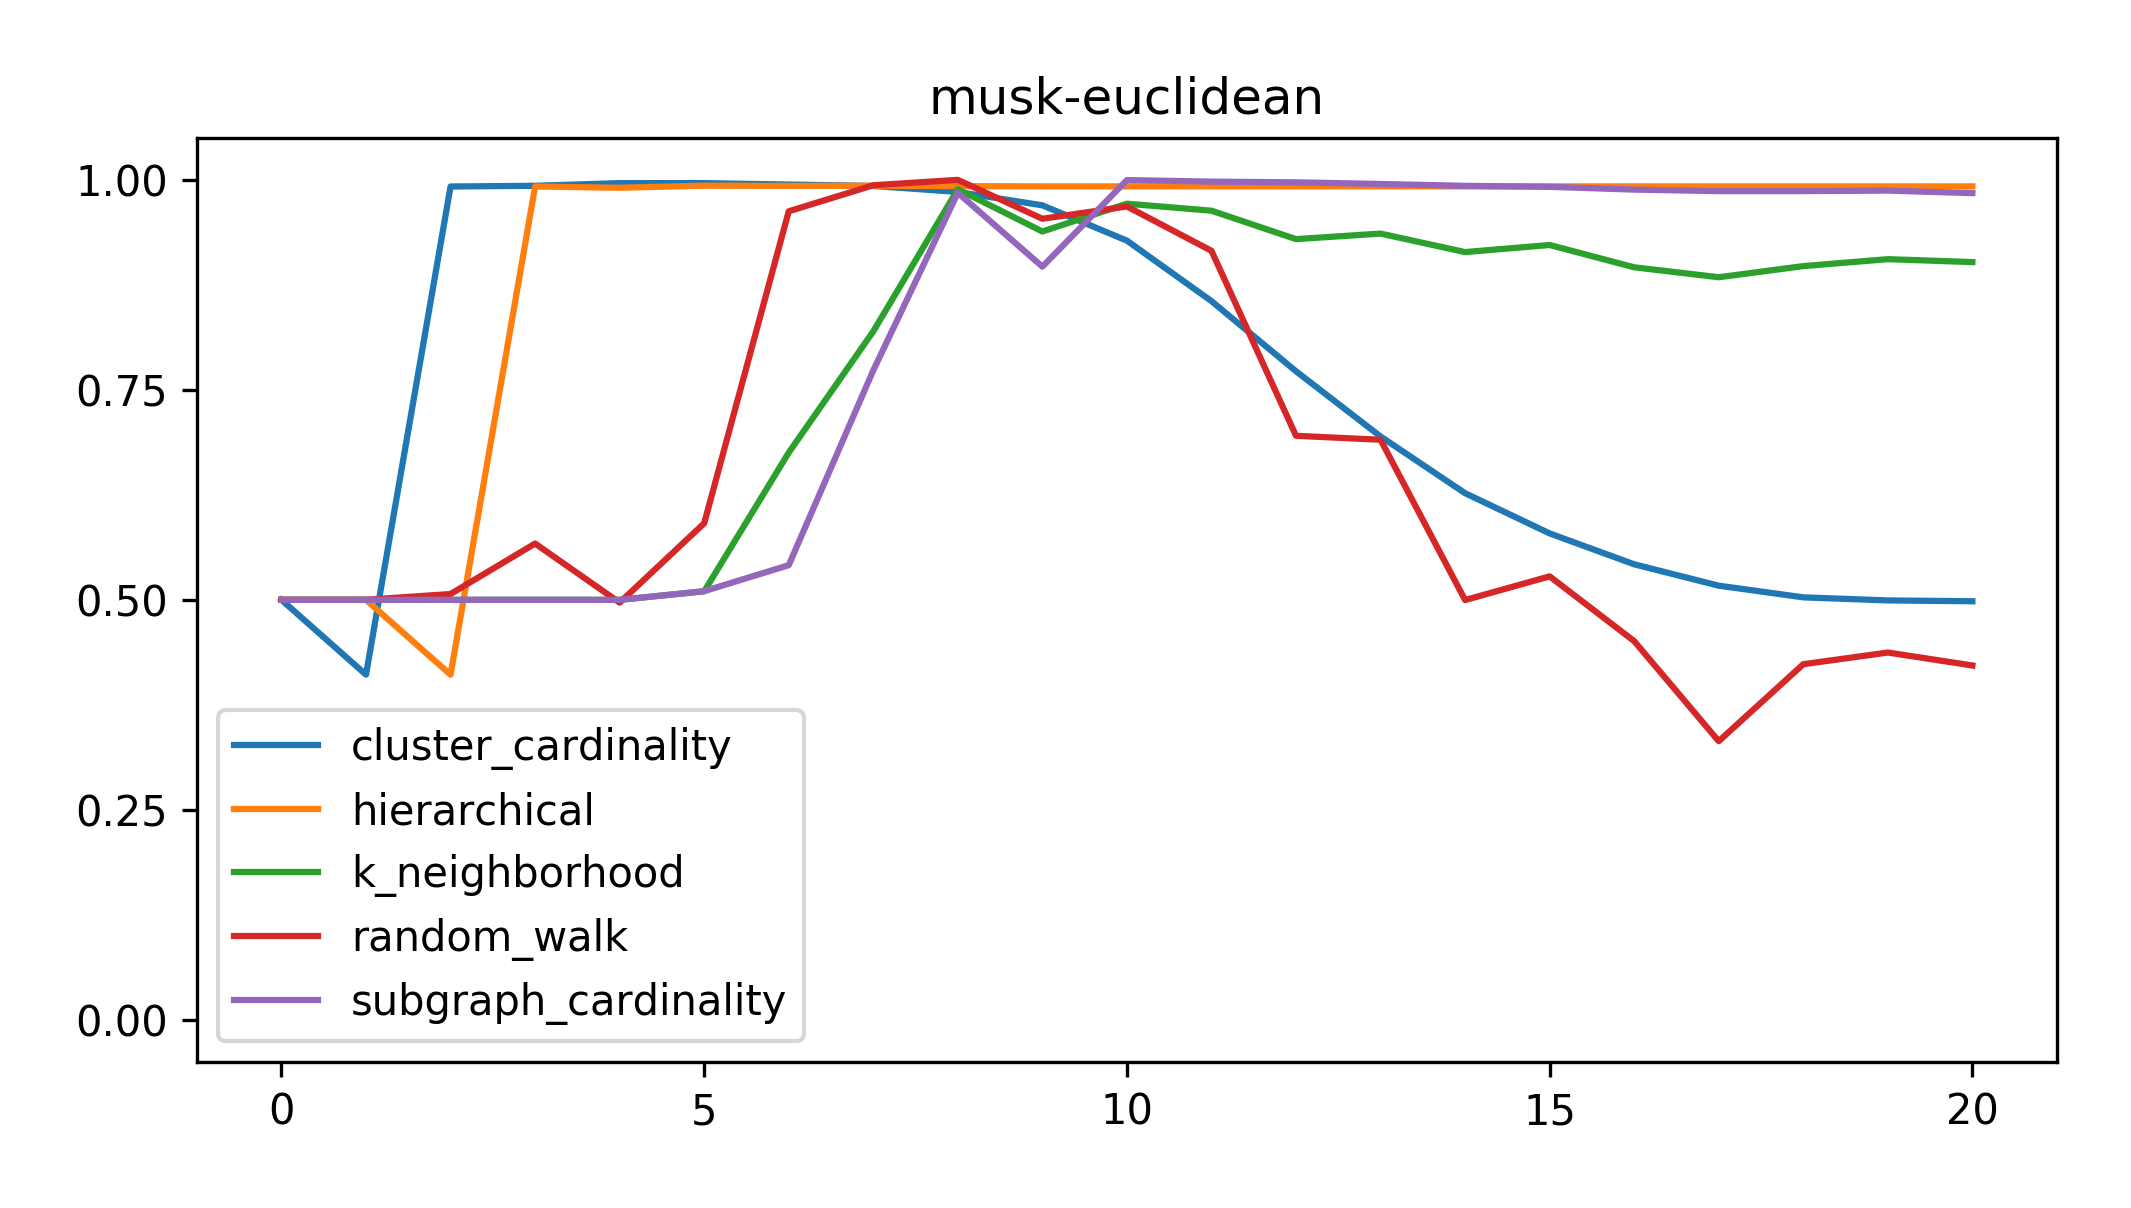
\includegraphics[width=2.2in]{kdd/static/auc_vs_depth/musk-euclidean.png}
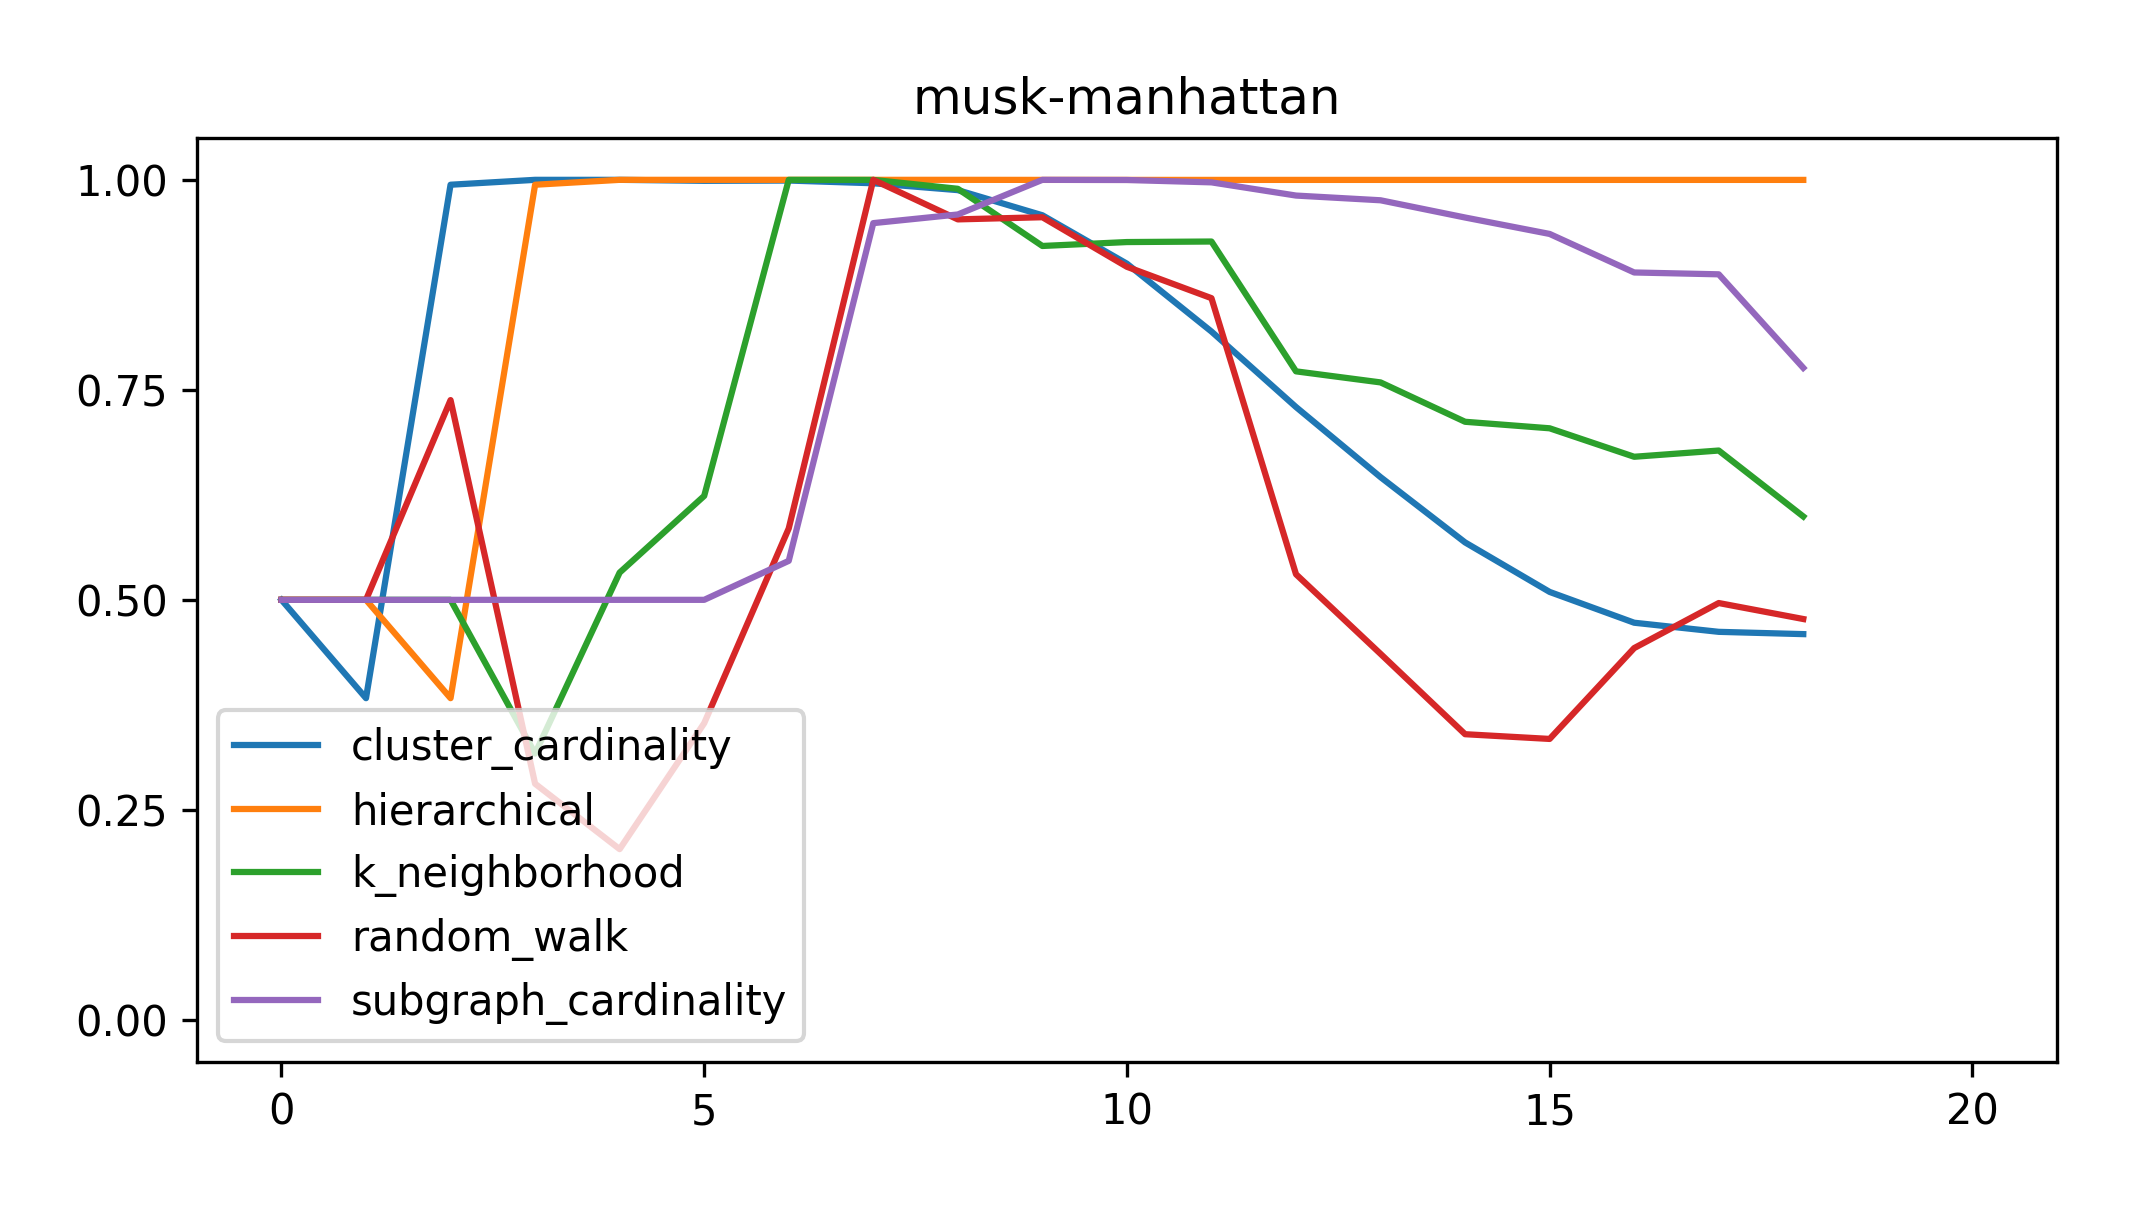
\includegraphics[width=2.2in]{kdd/static/auc_vs_depth/musk-manhattan.png}

% Optdigits
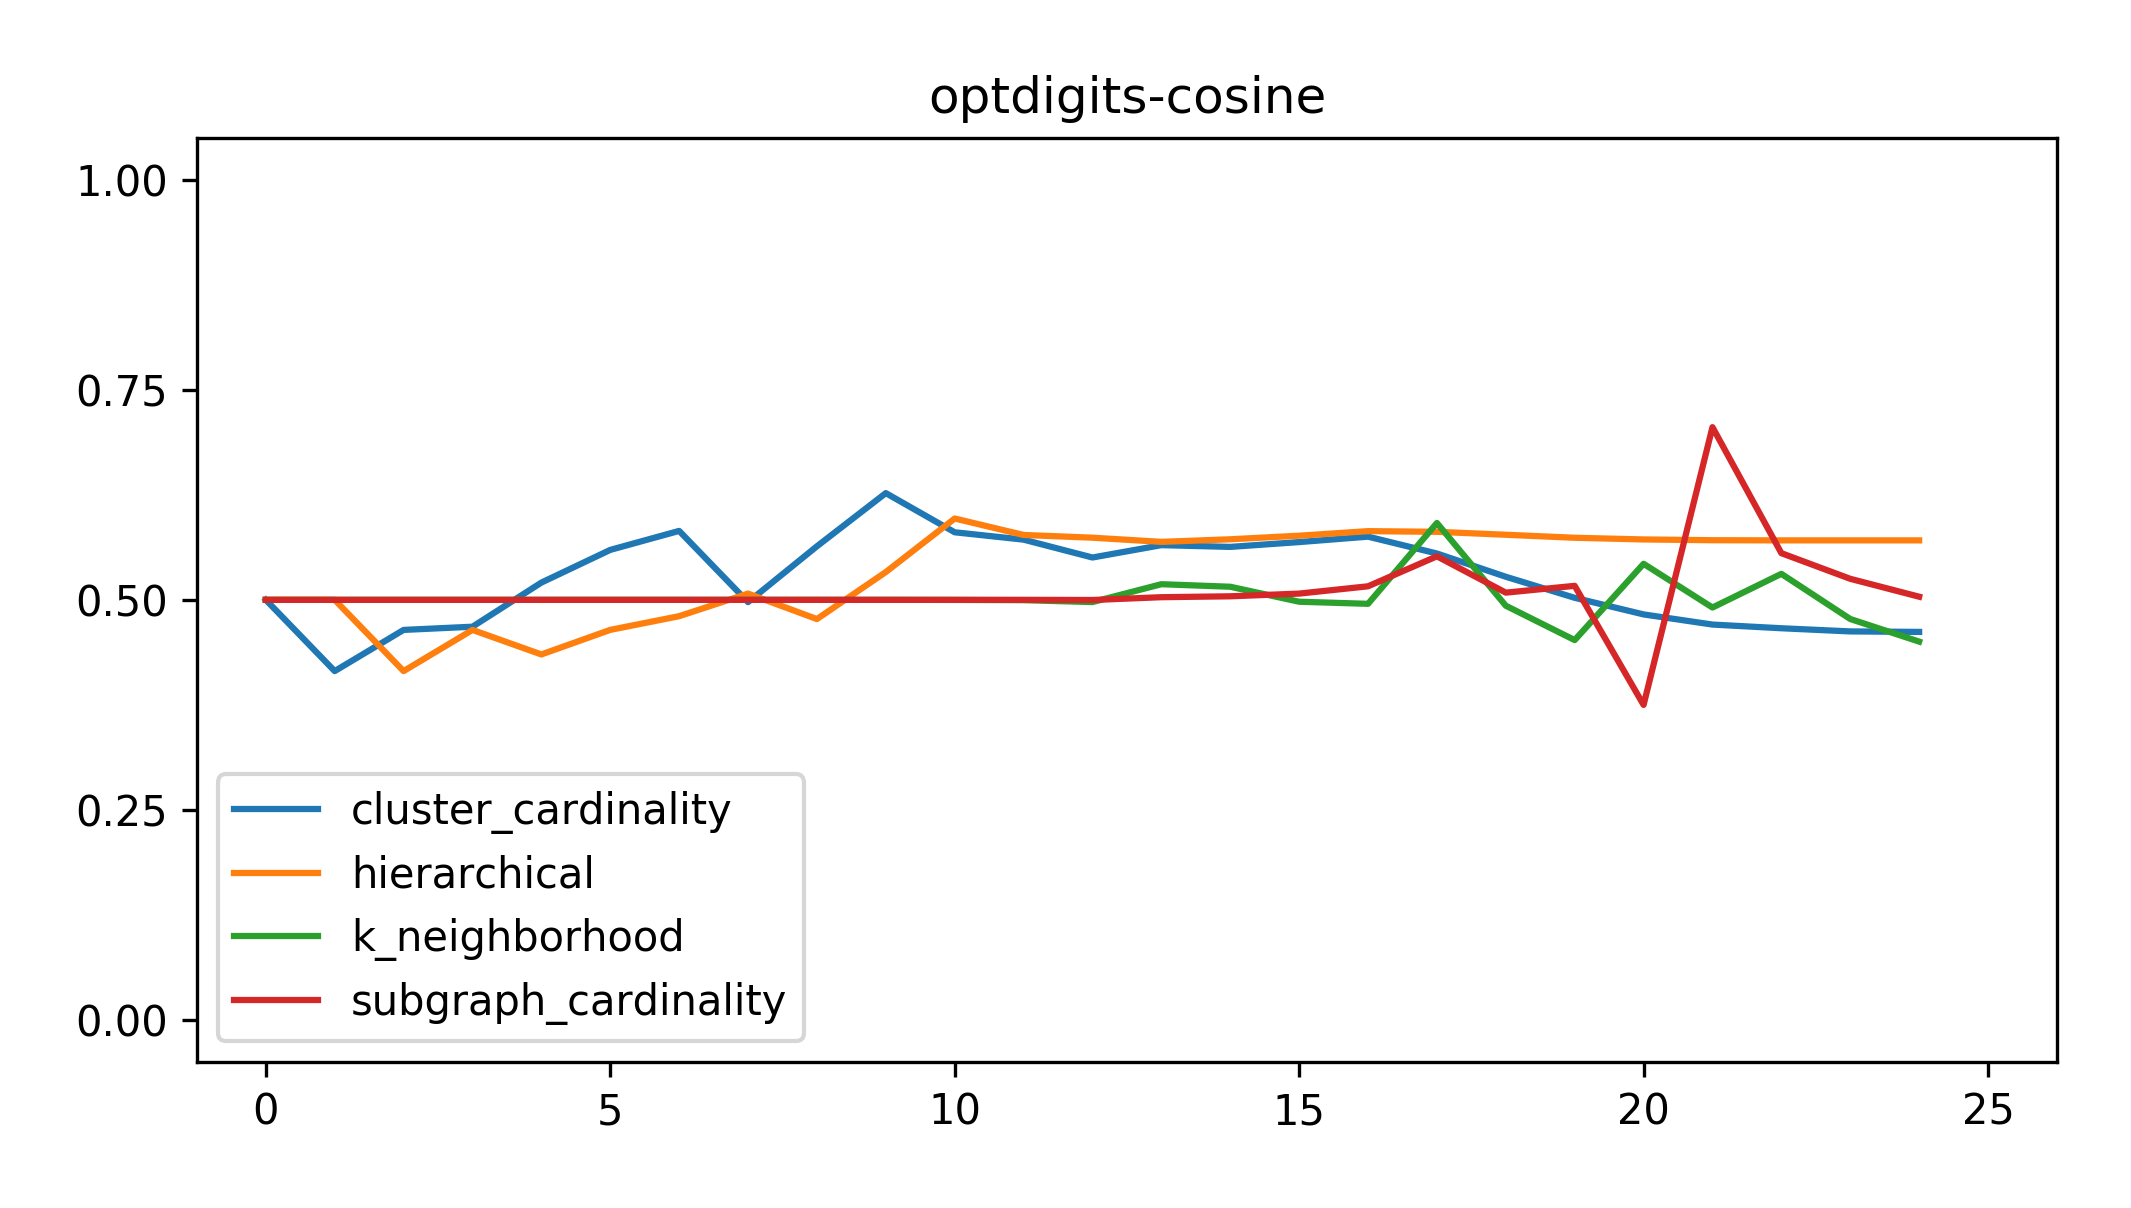
\includegraphics[width=2.2in]{kdd/static/auc_vs_depth/optdigits-cosine.png}
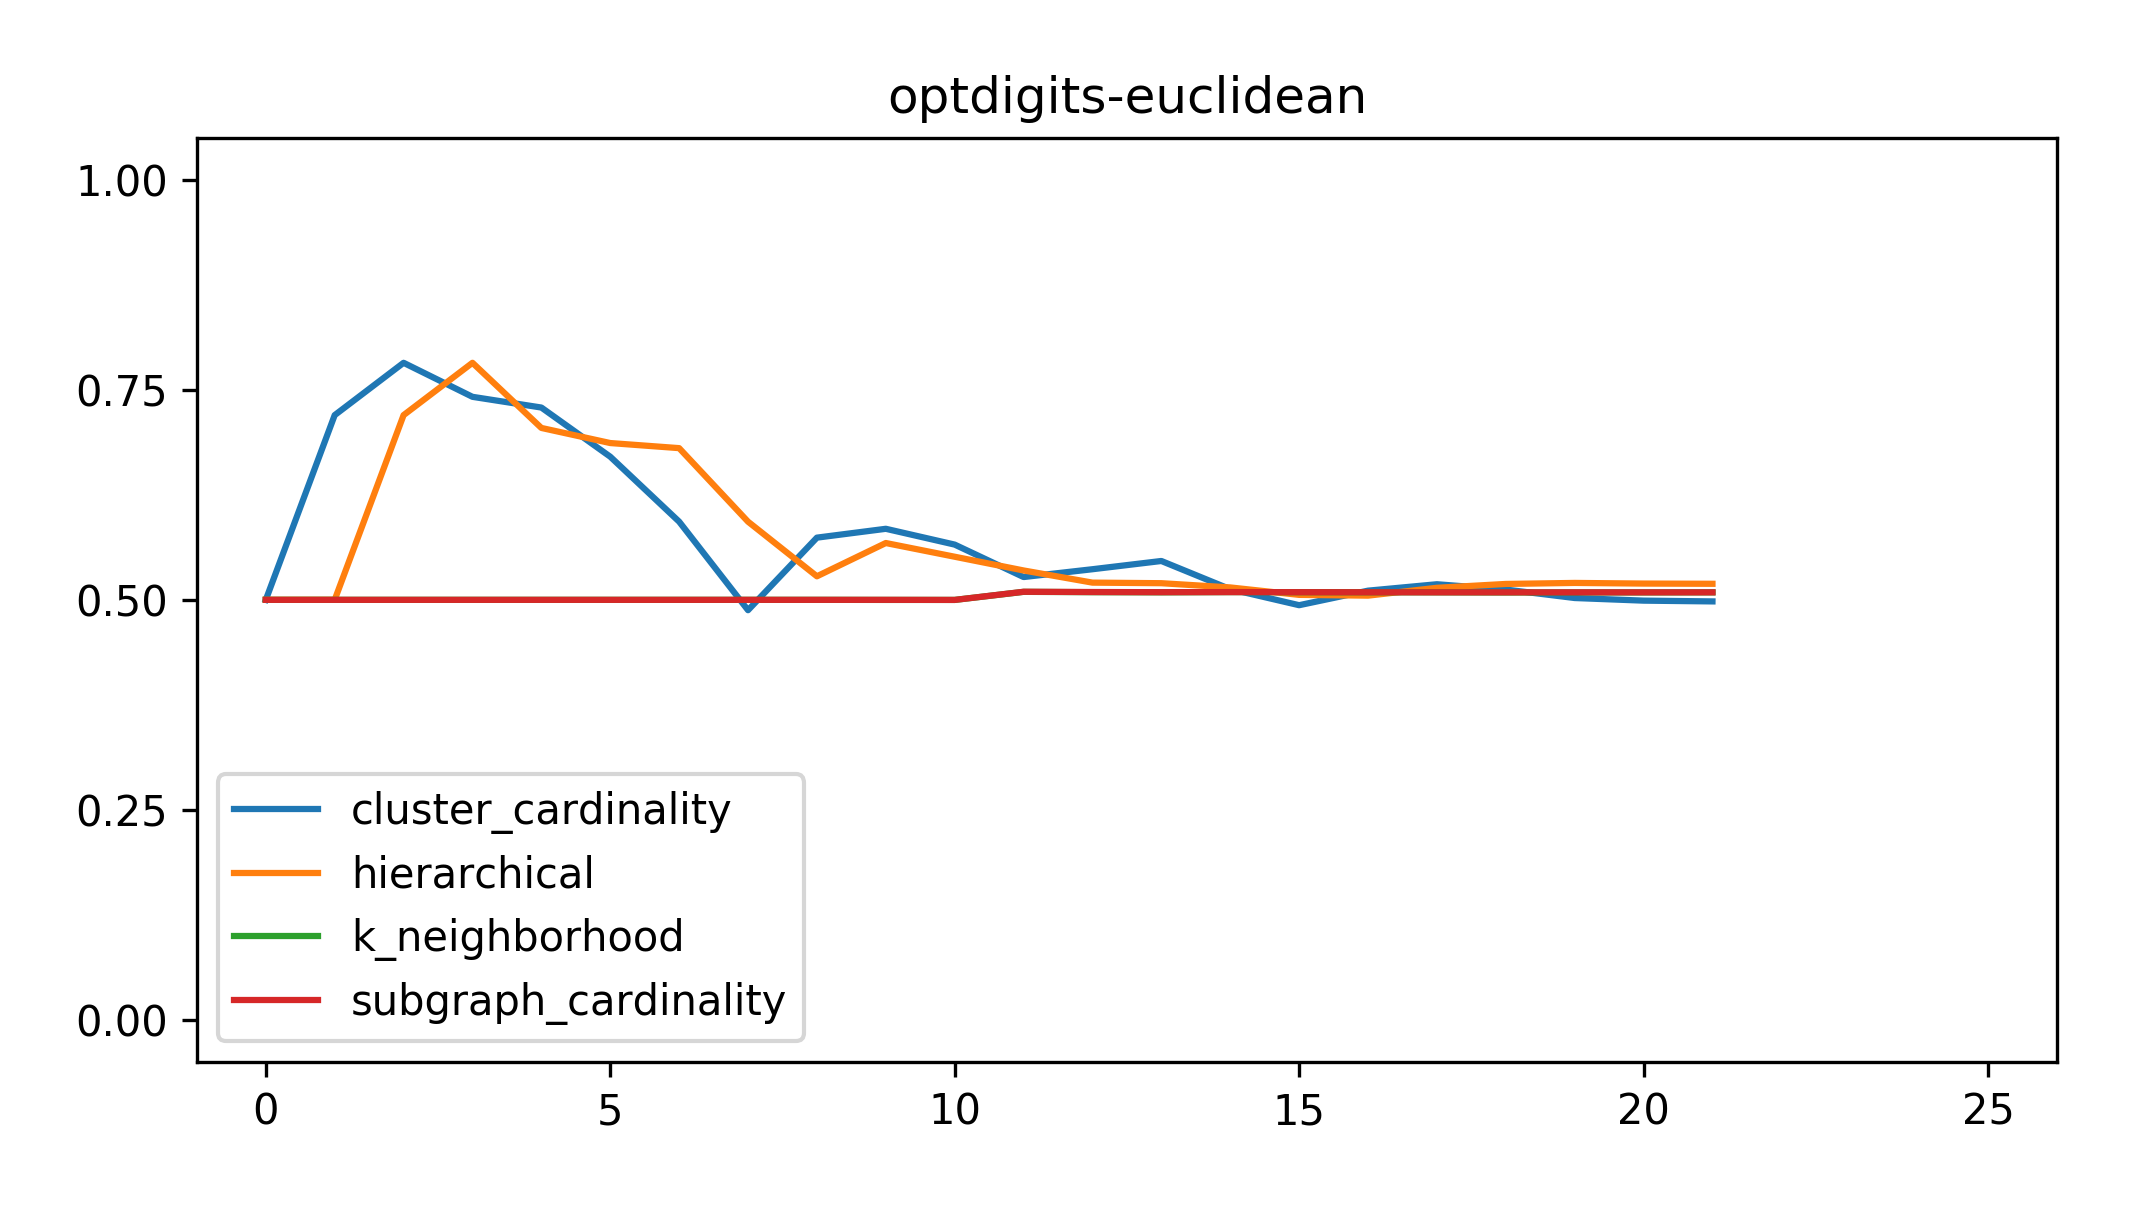
\includegraphics[width=2.2in]{kdd/static/auc_vs_depth/optdigits-euclidean.png}
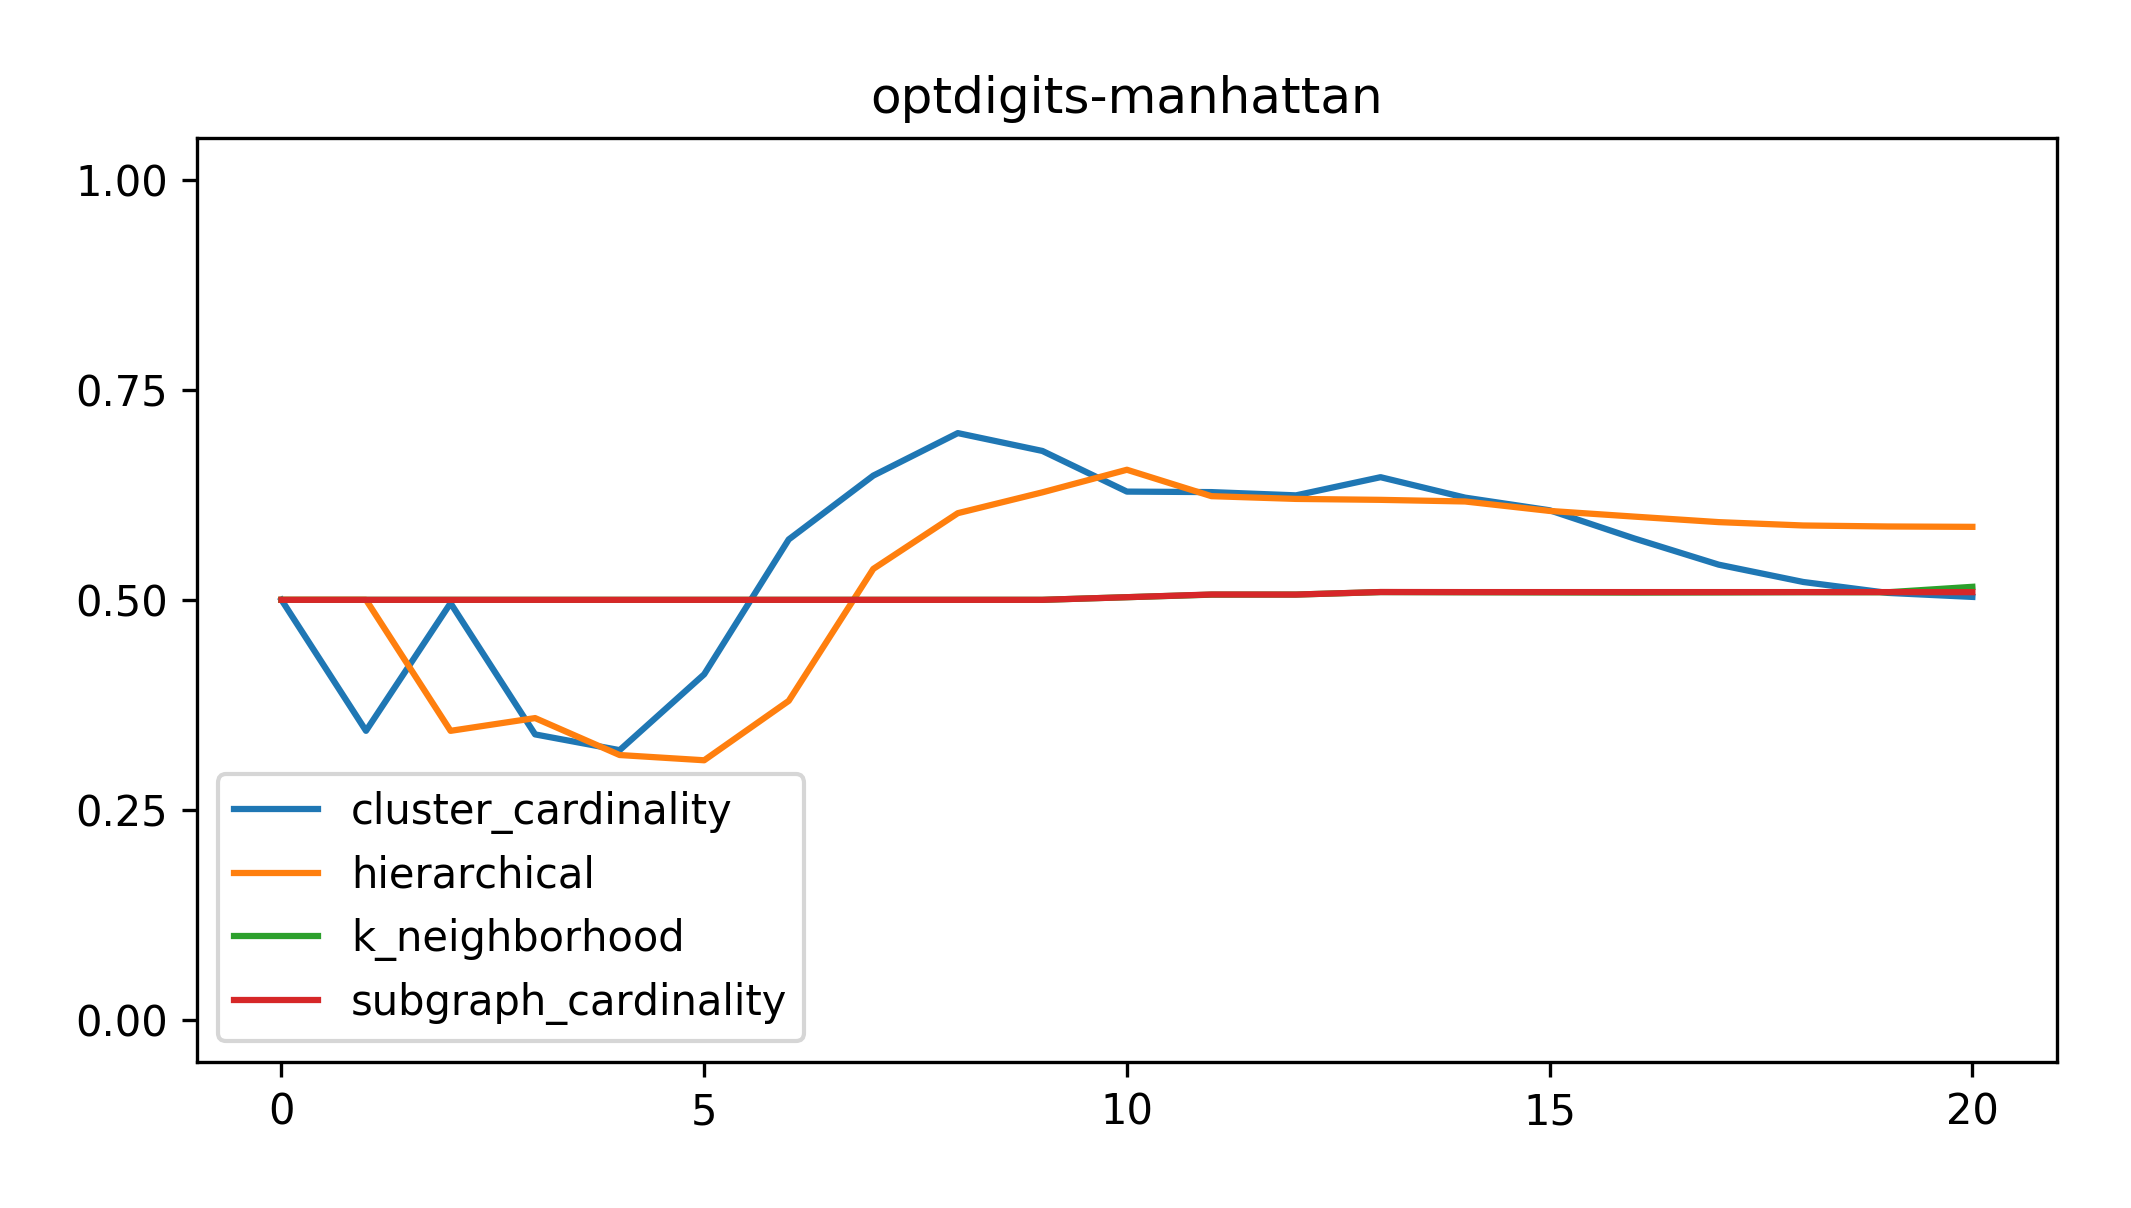
\includegraphics[width=2.2in]{kdd/static/auc_vs_depth/optdigits-manhattan.png}

% Pima
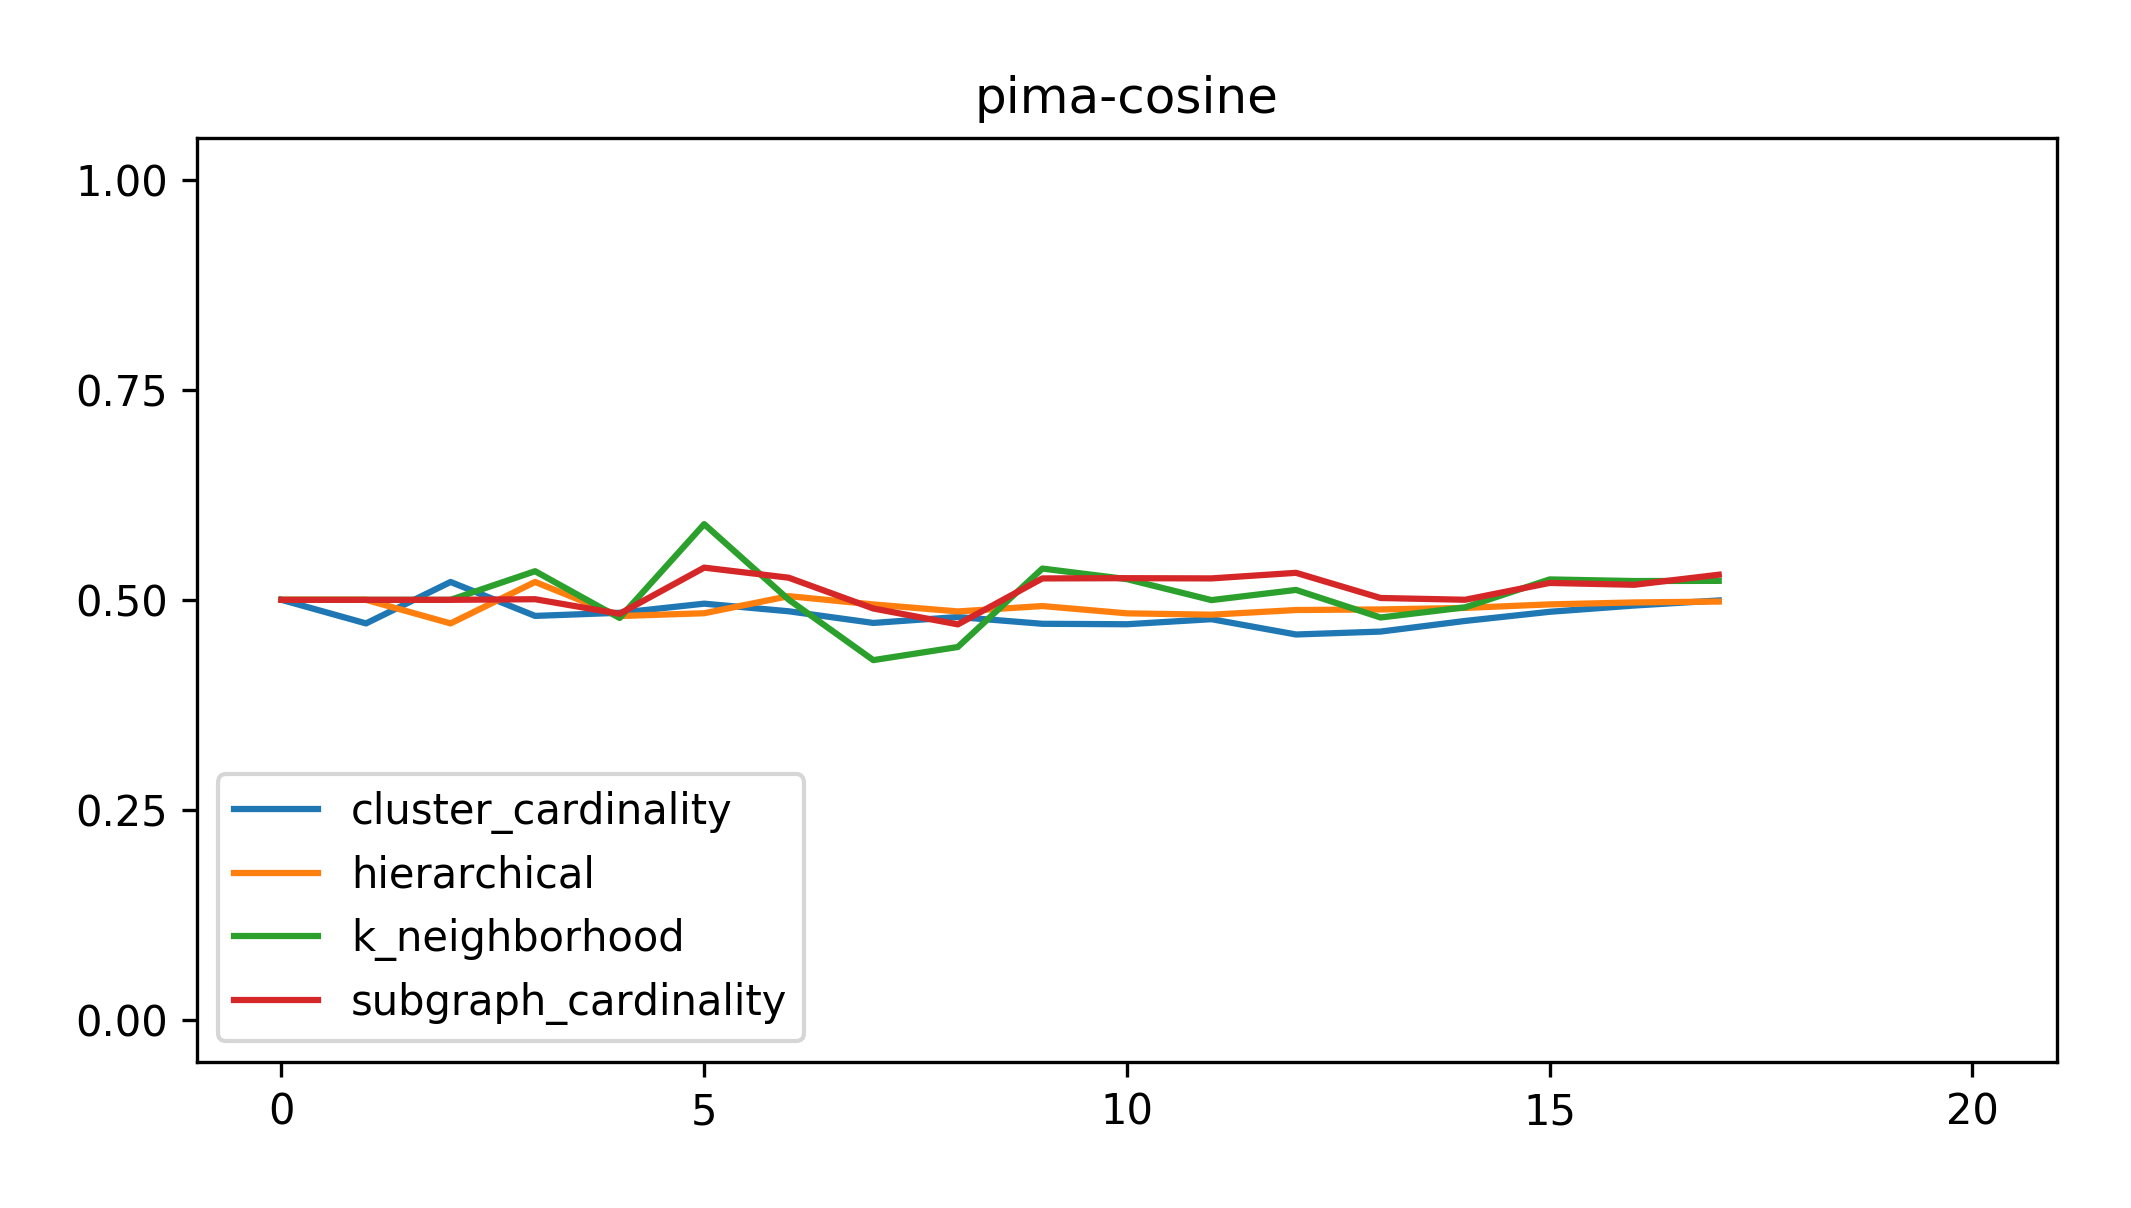
\includegraphics[width=2.2in]{kdd/static/auc_vs_depth/pima-cosine.png}
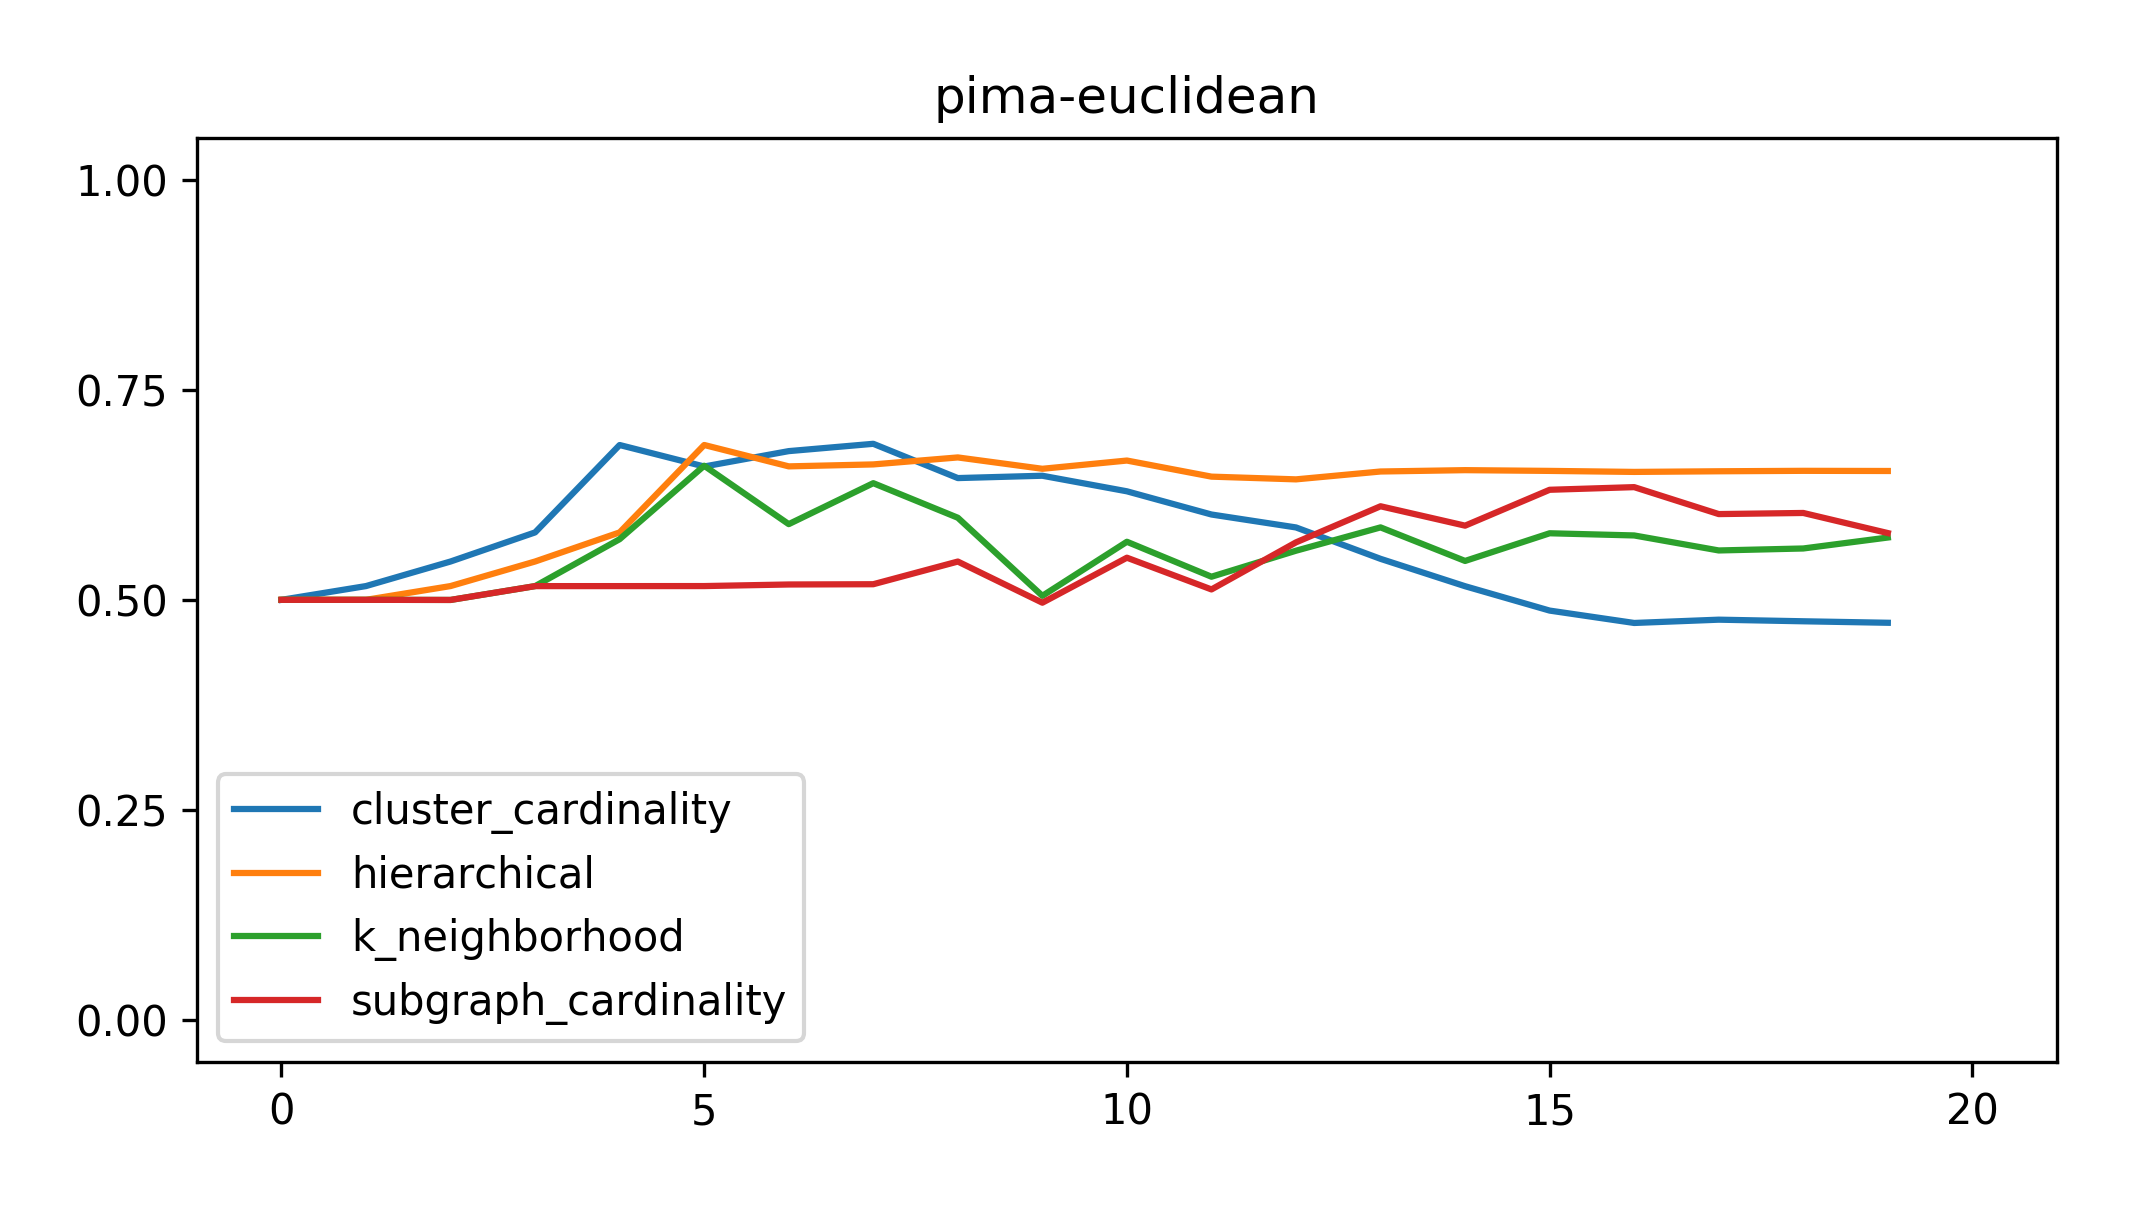
\includegraphics[width=2.2in]{kdd/static/auc_vs_depth/pima-euclidean.png}
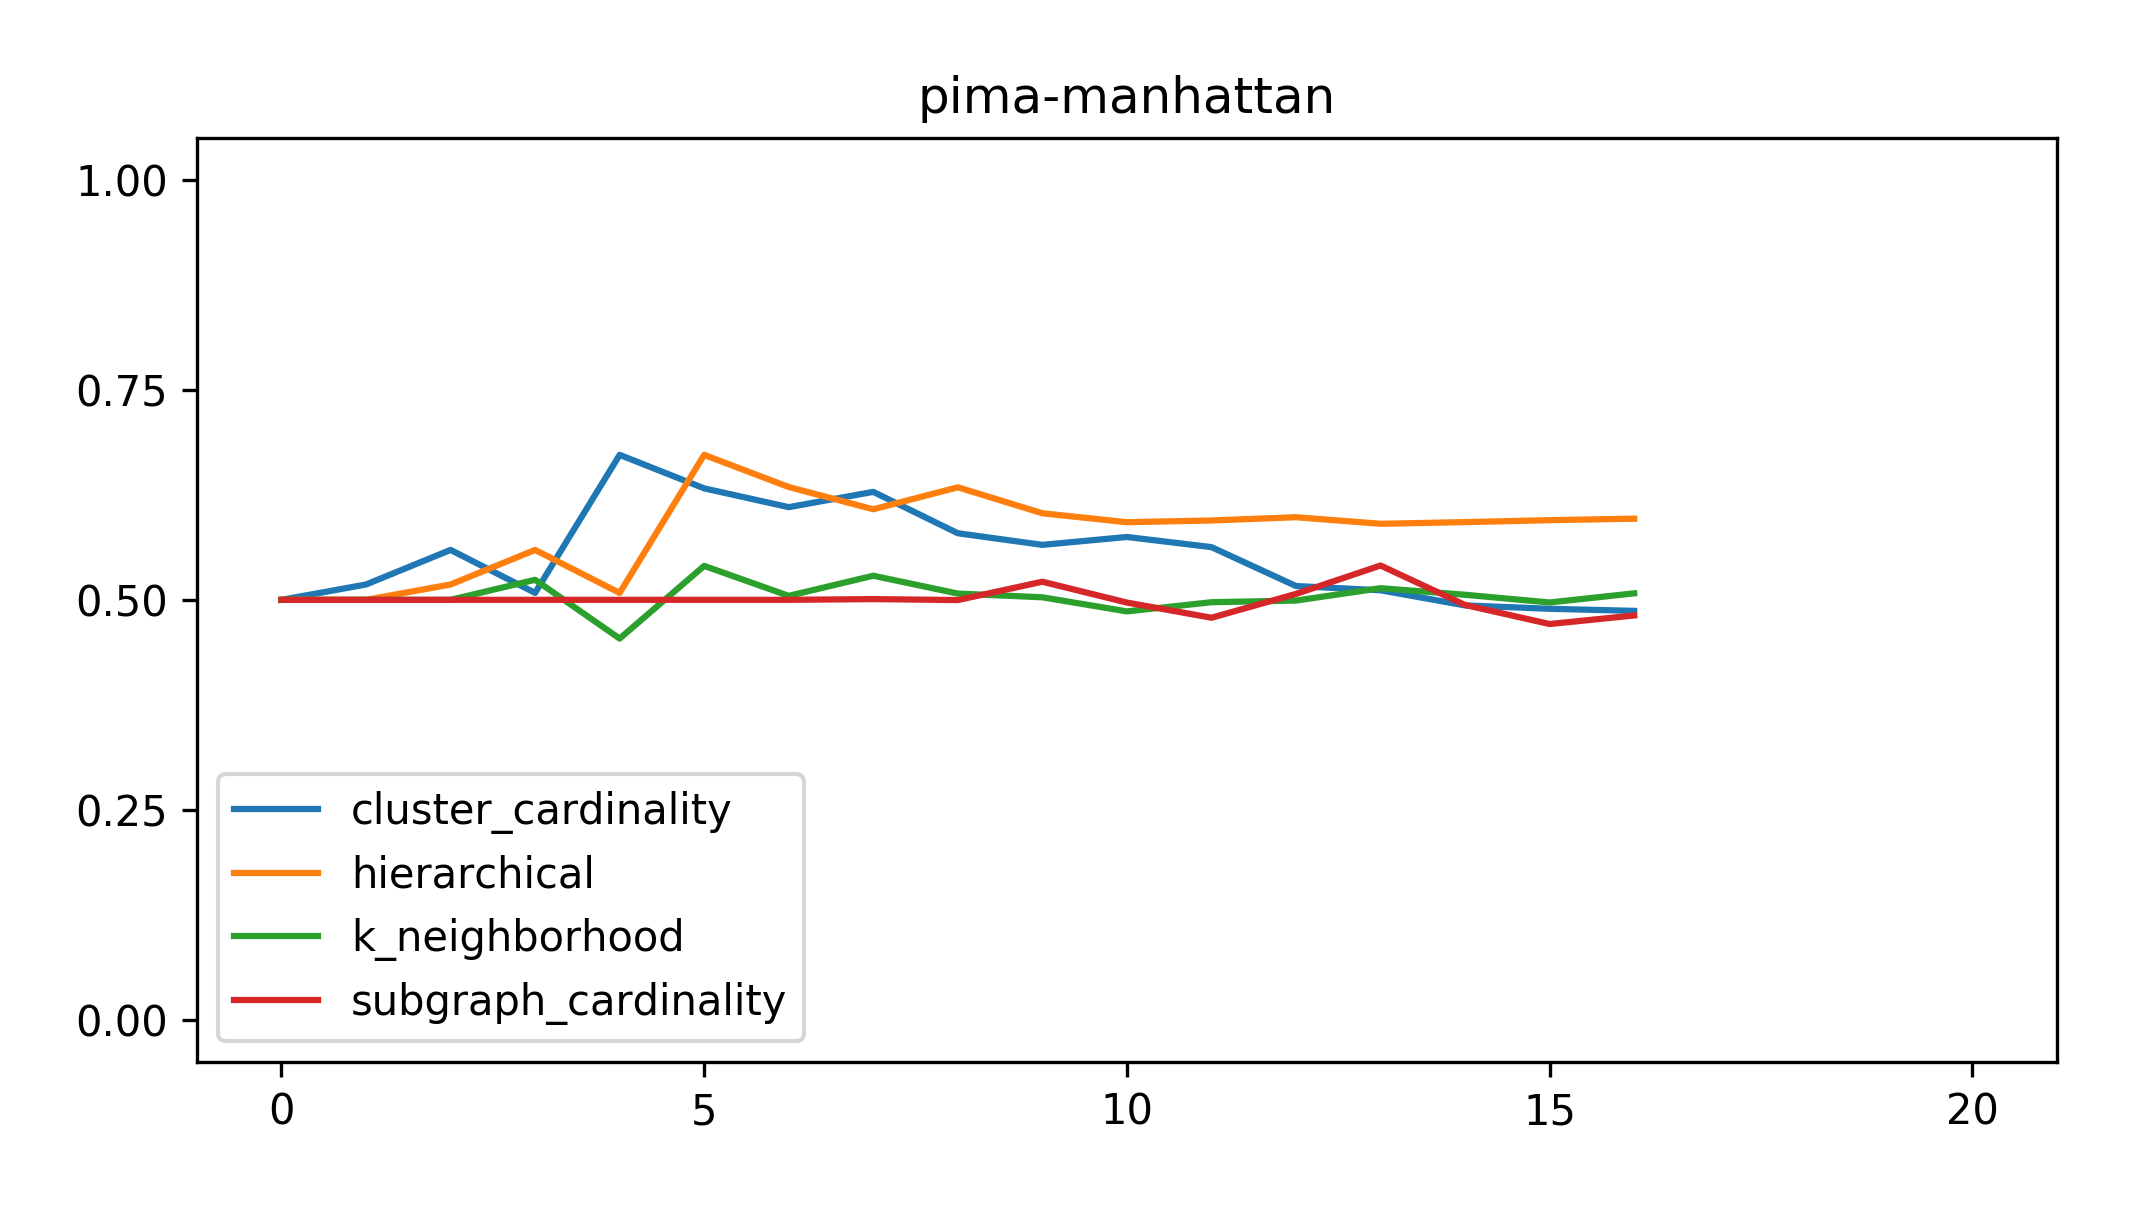
\includegraphics[width=2.2in]{kdd/static/auc_vs_depth/pima-manhattan.png}

% Satellite
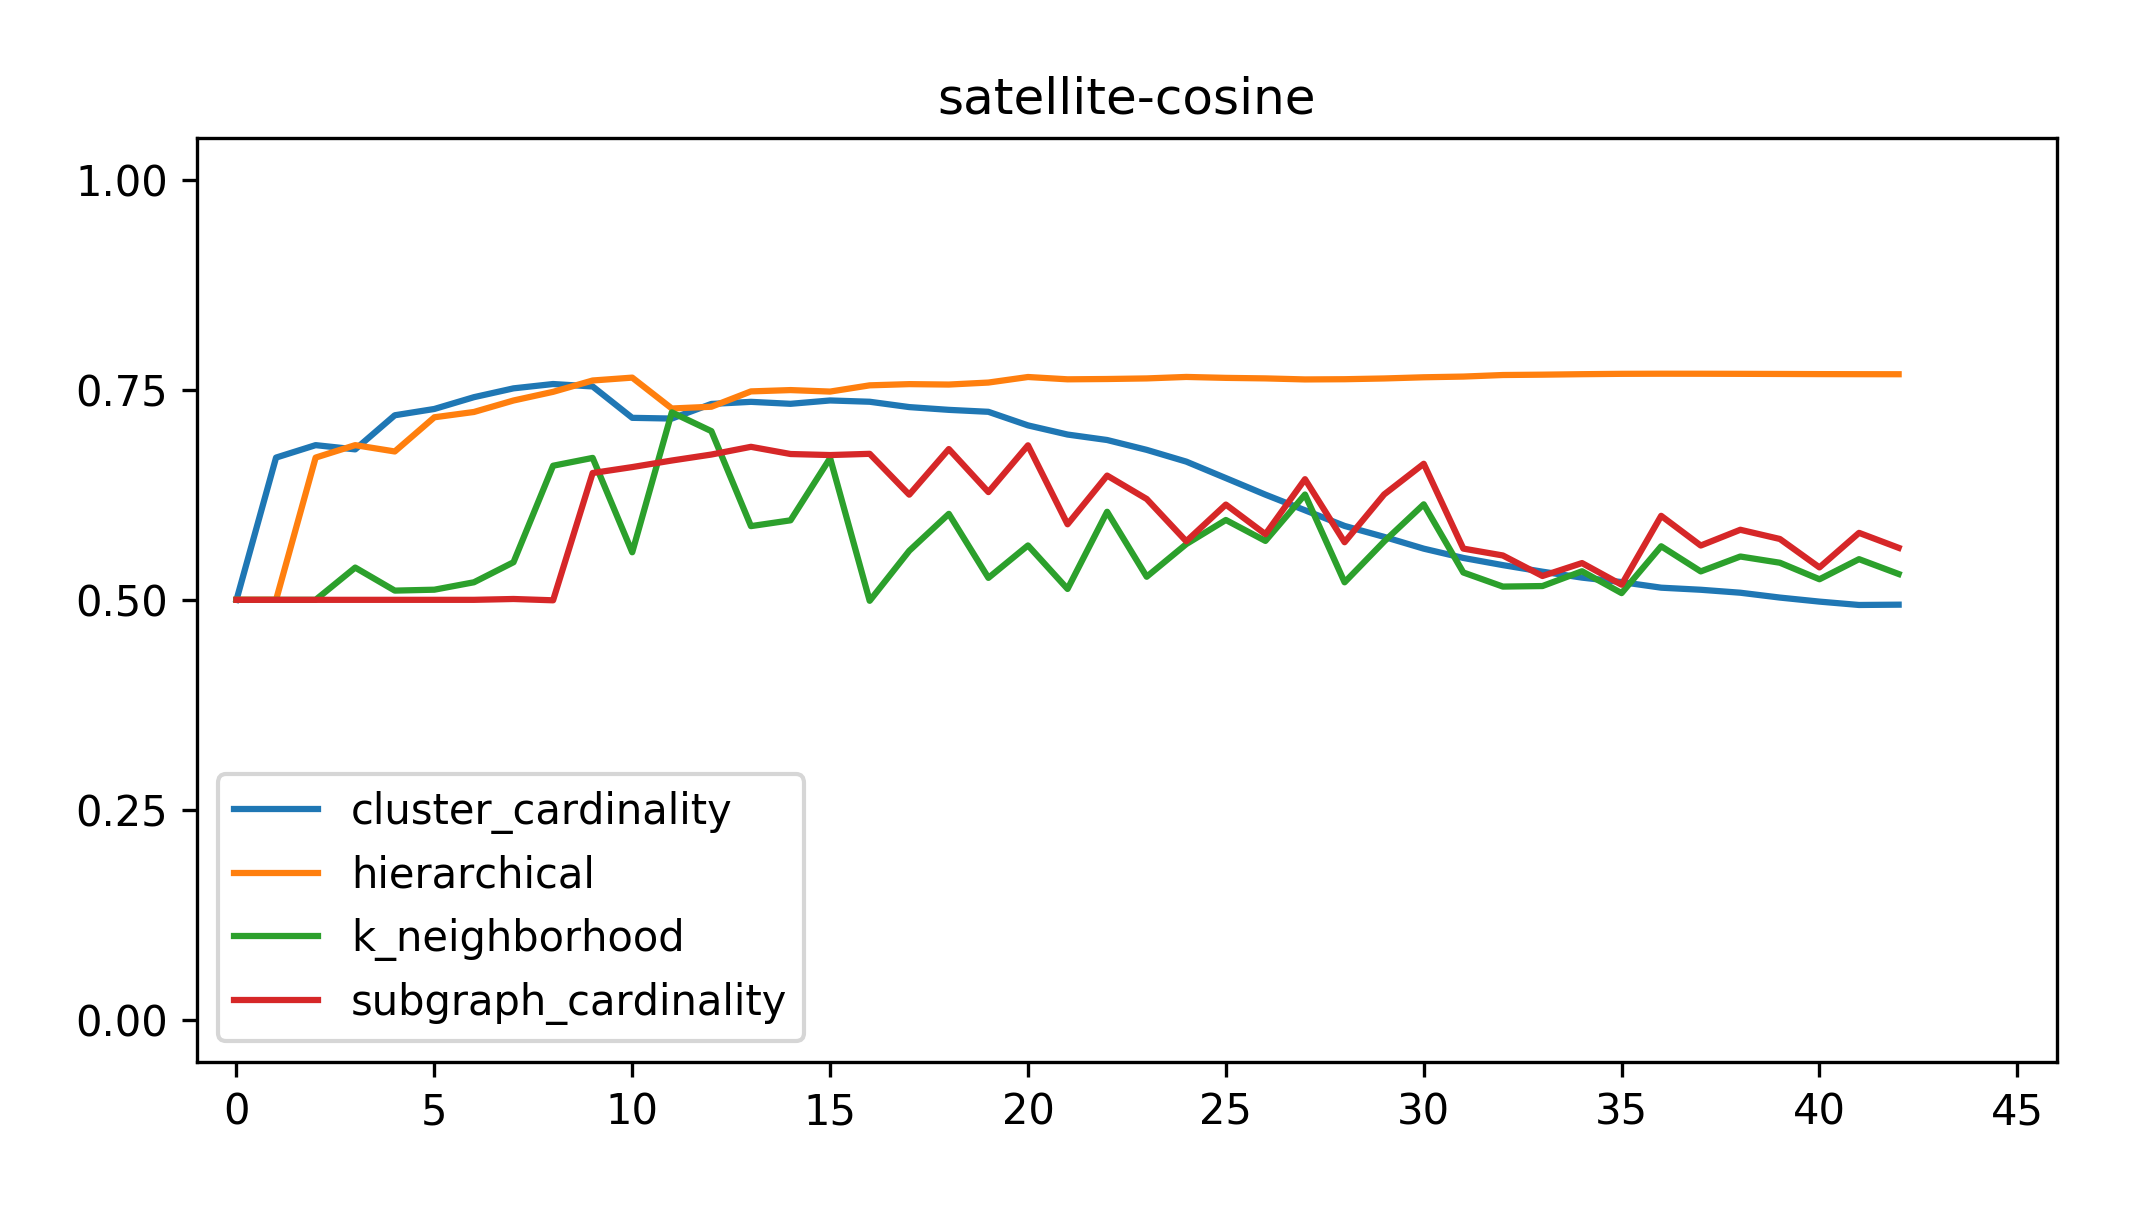
\includegraphics[width=2.2in]{kdd/static/auc_vs_depth/satellite-cosine.png}
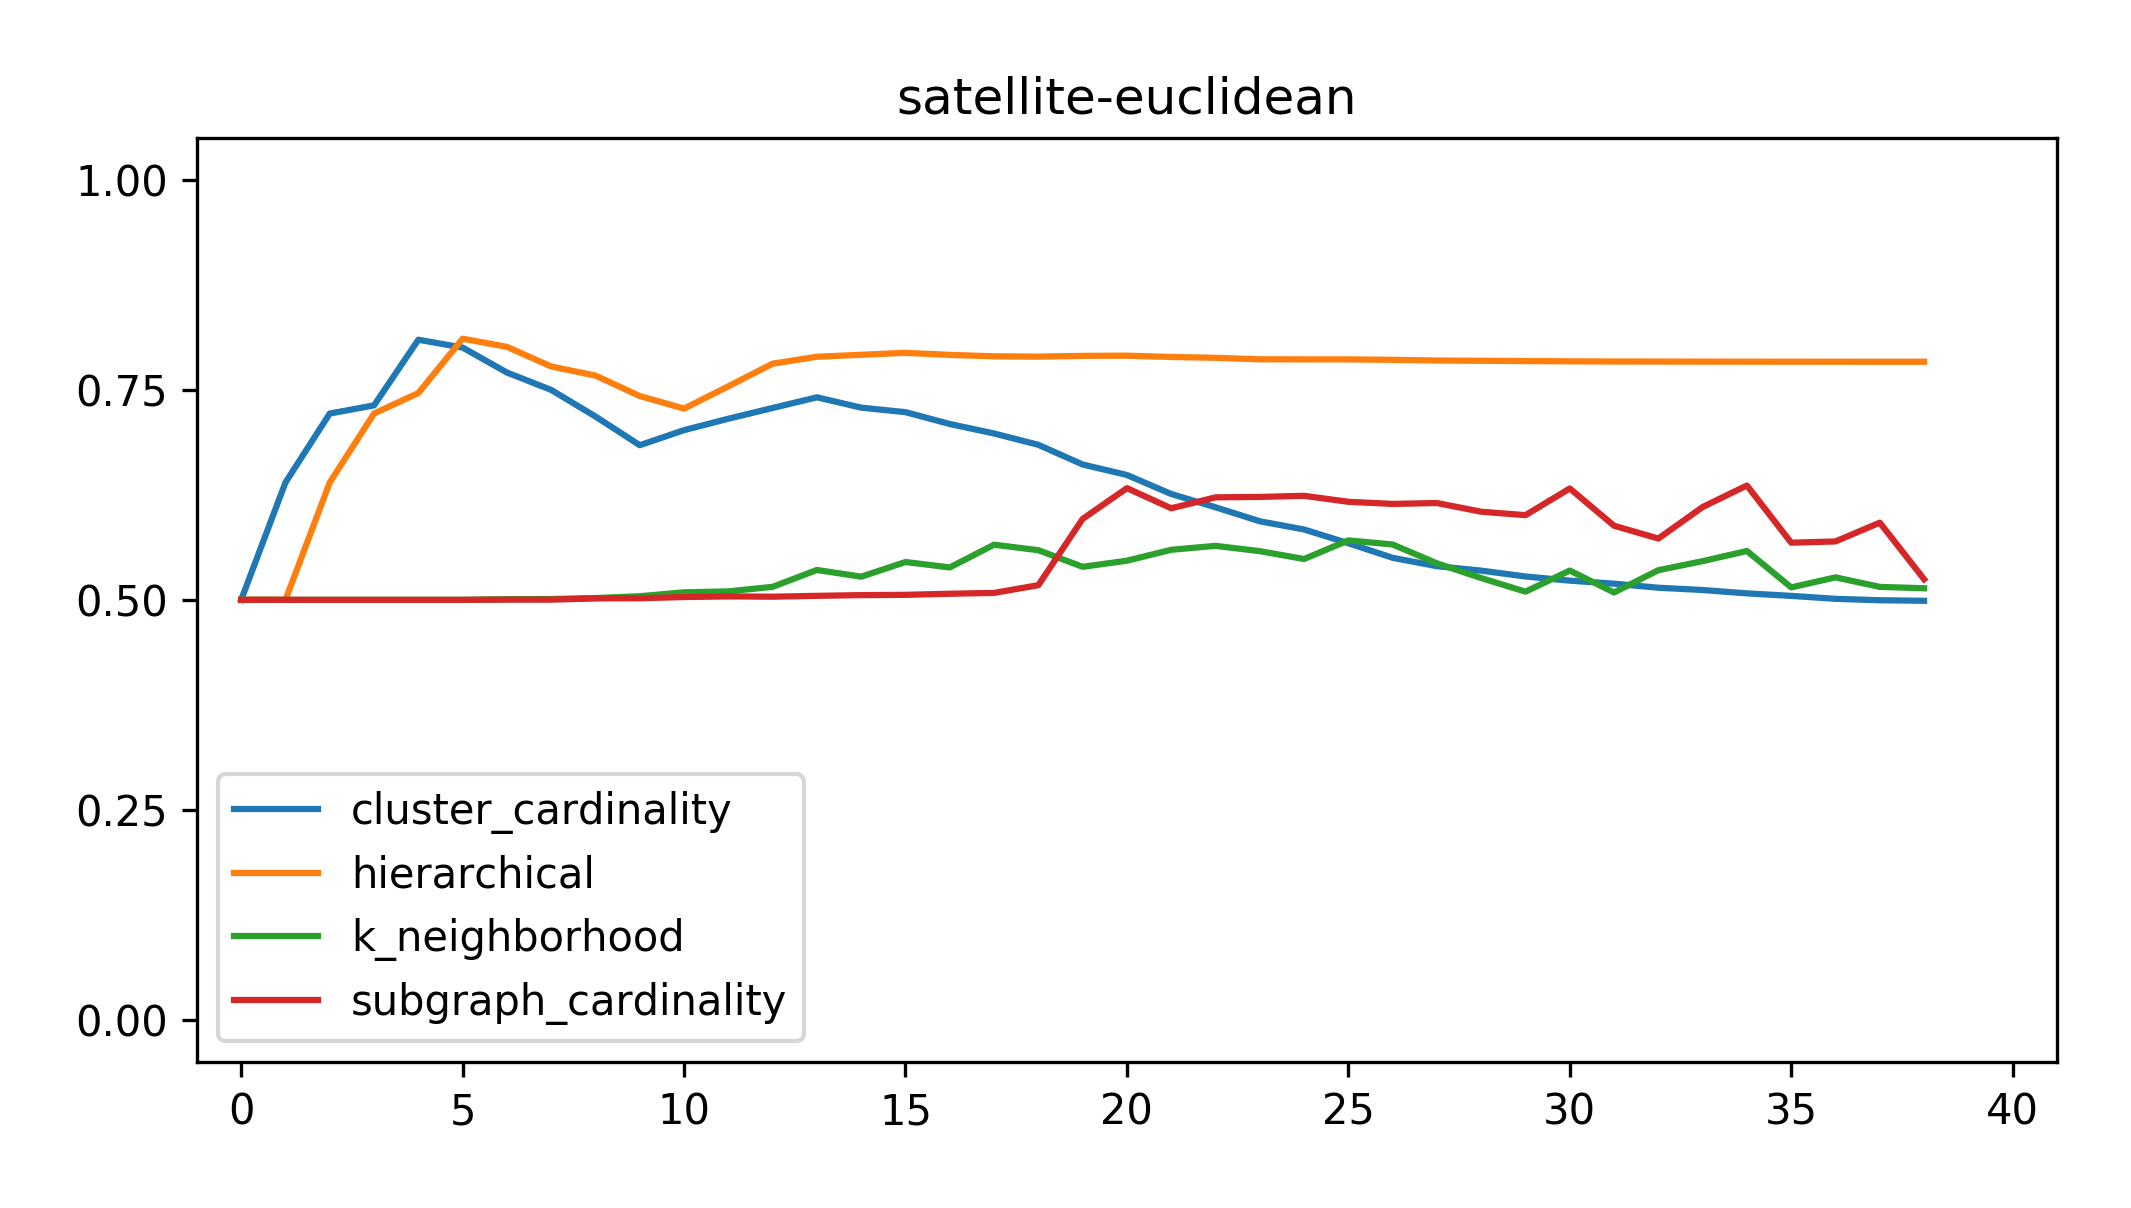
\includegraphics[width=2.2in]{kdd/static/auc_vs_depth/satellite-euclidean.png}
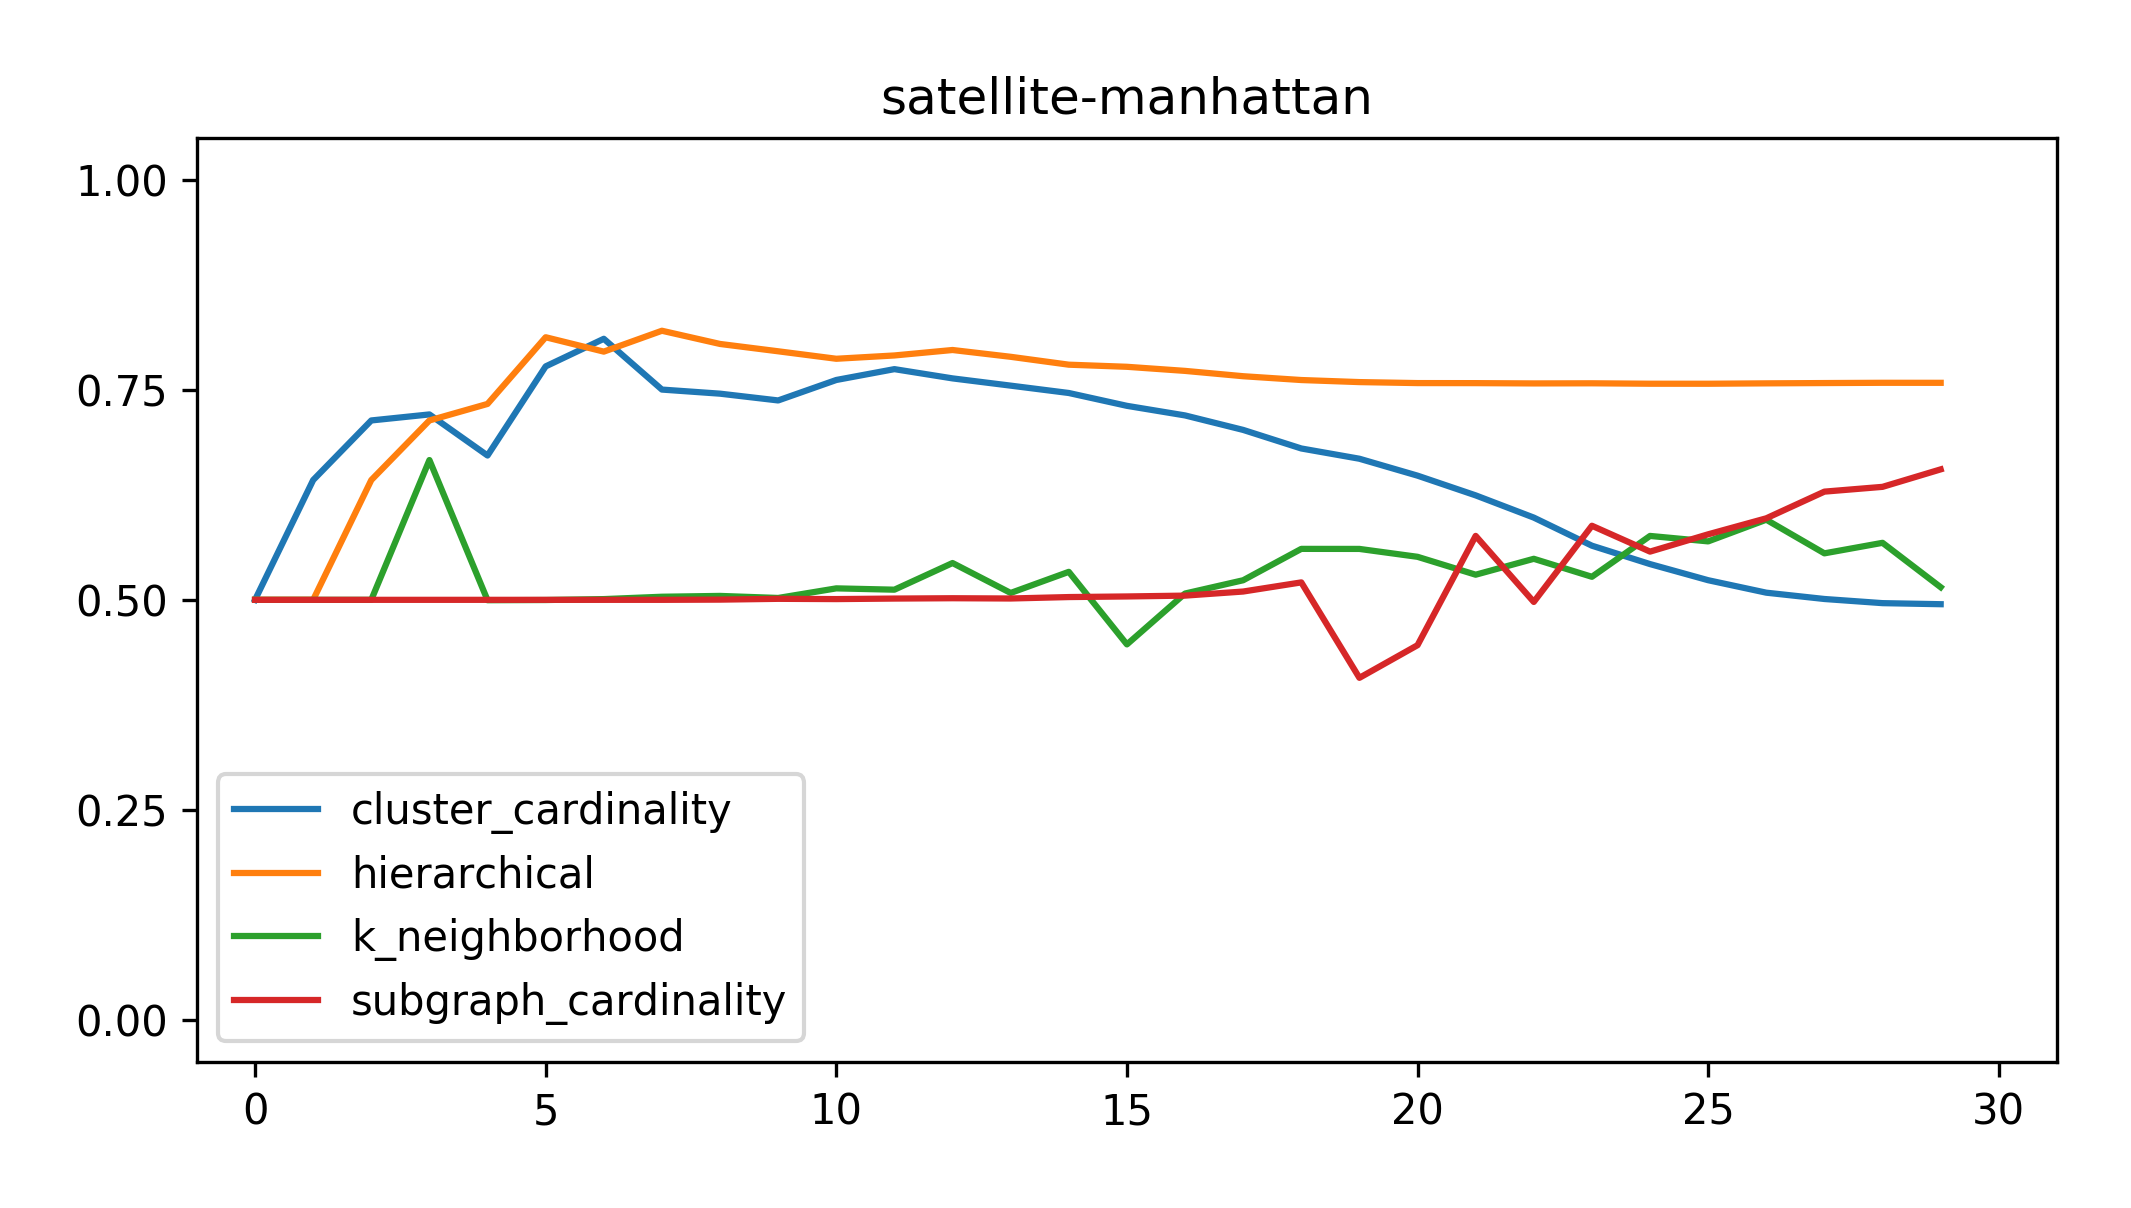
\includegraphics[width=2.2in]{kdd/static/auc_vs_depth/satellite-manhattan.png}

\caption{
Plots of ROC-AUC vs Depth for our mearures of Anomolousness.
}

\label{results:datasets_2}
\end{figure*}

\begin{figure*}[!t]
\centering
% Satimage-2
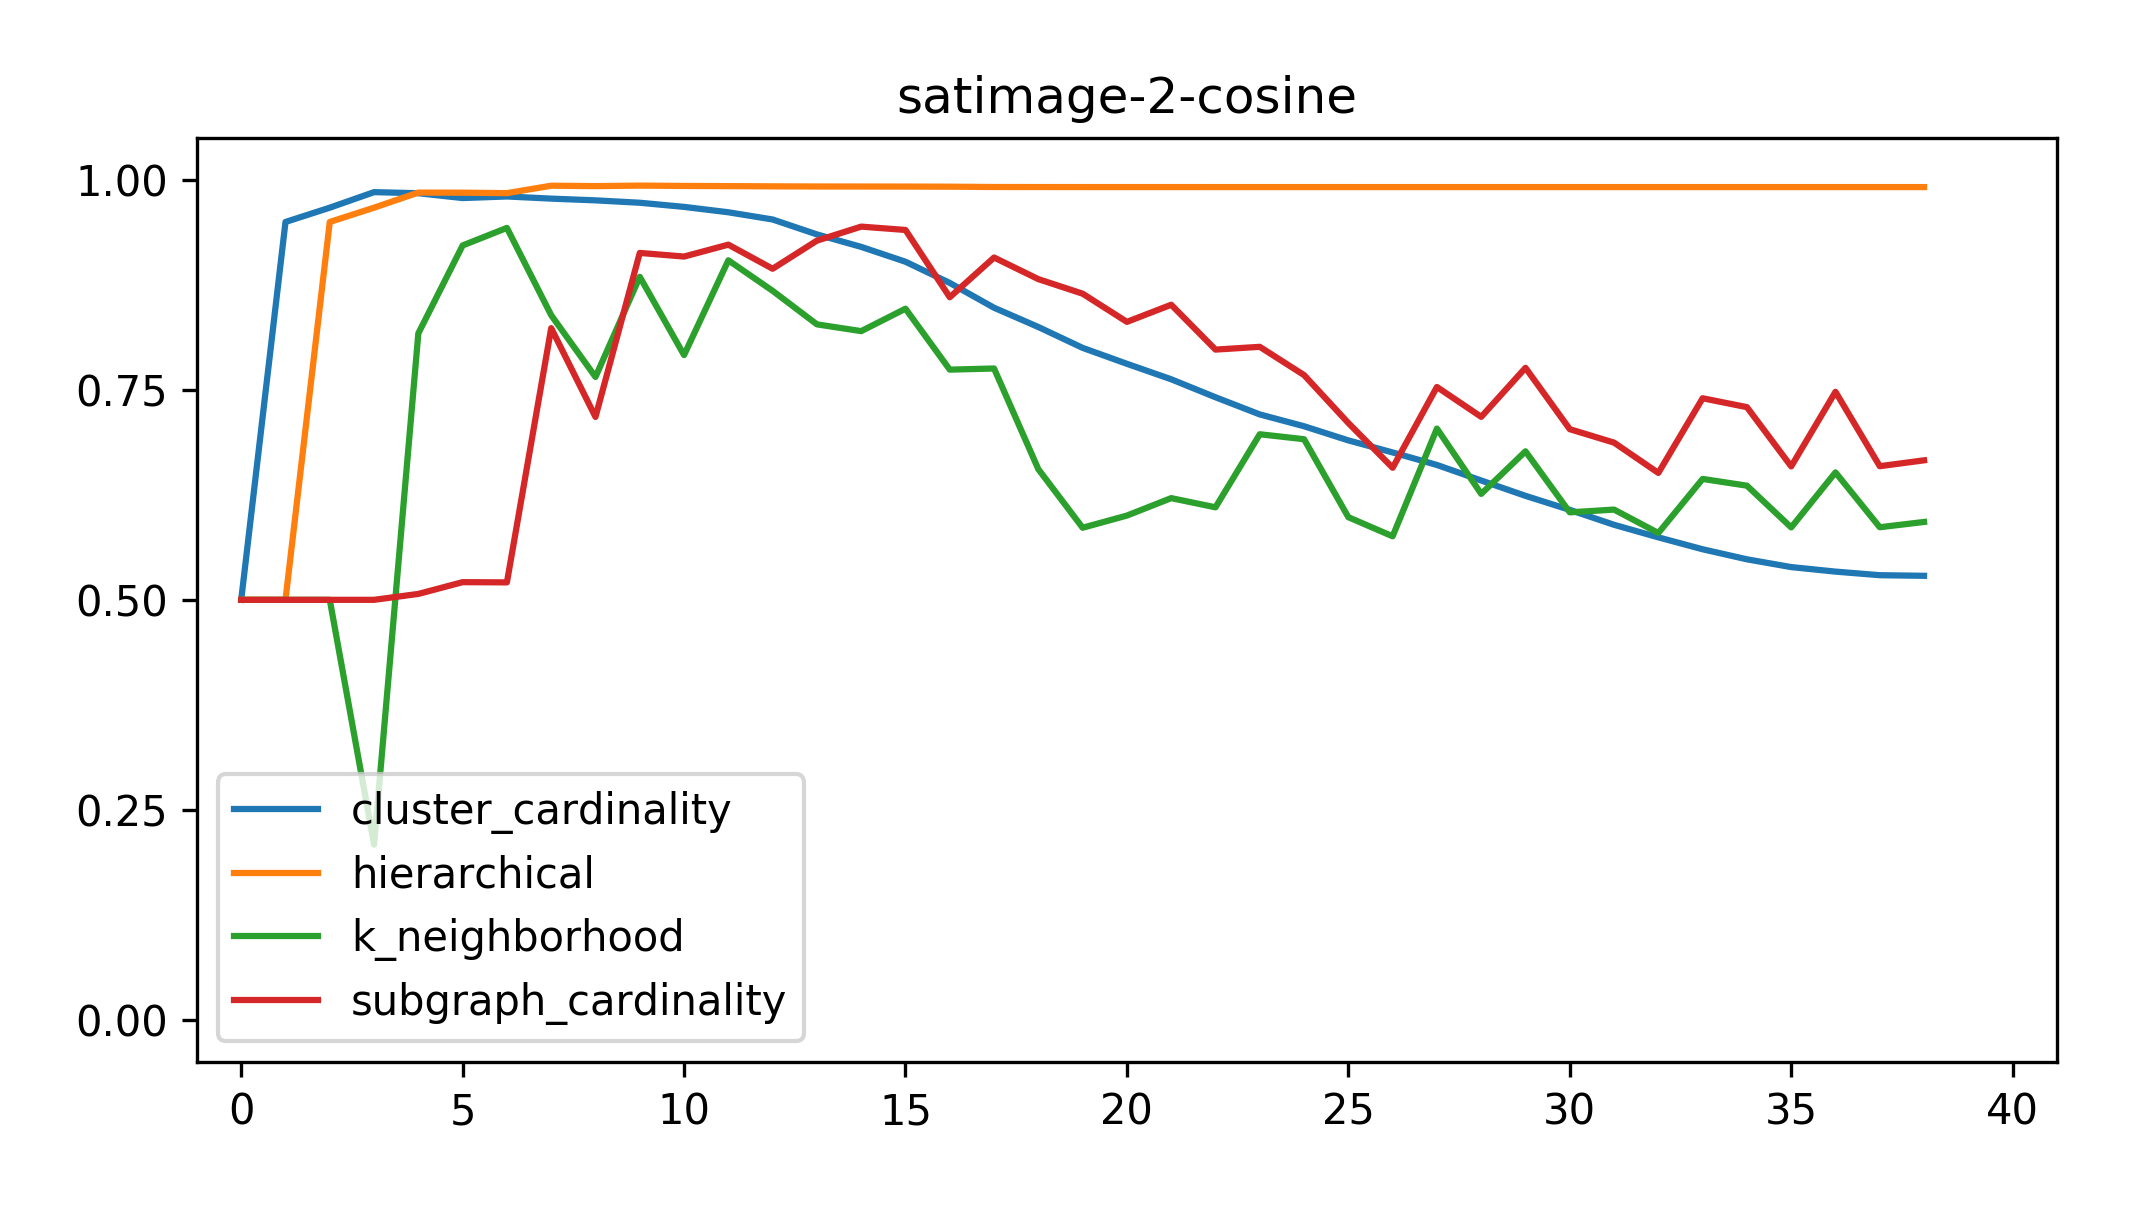
\includegraphics[width=2.2in]{kdd/static/auc_vs_depth/satimage-2-cosine.png}
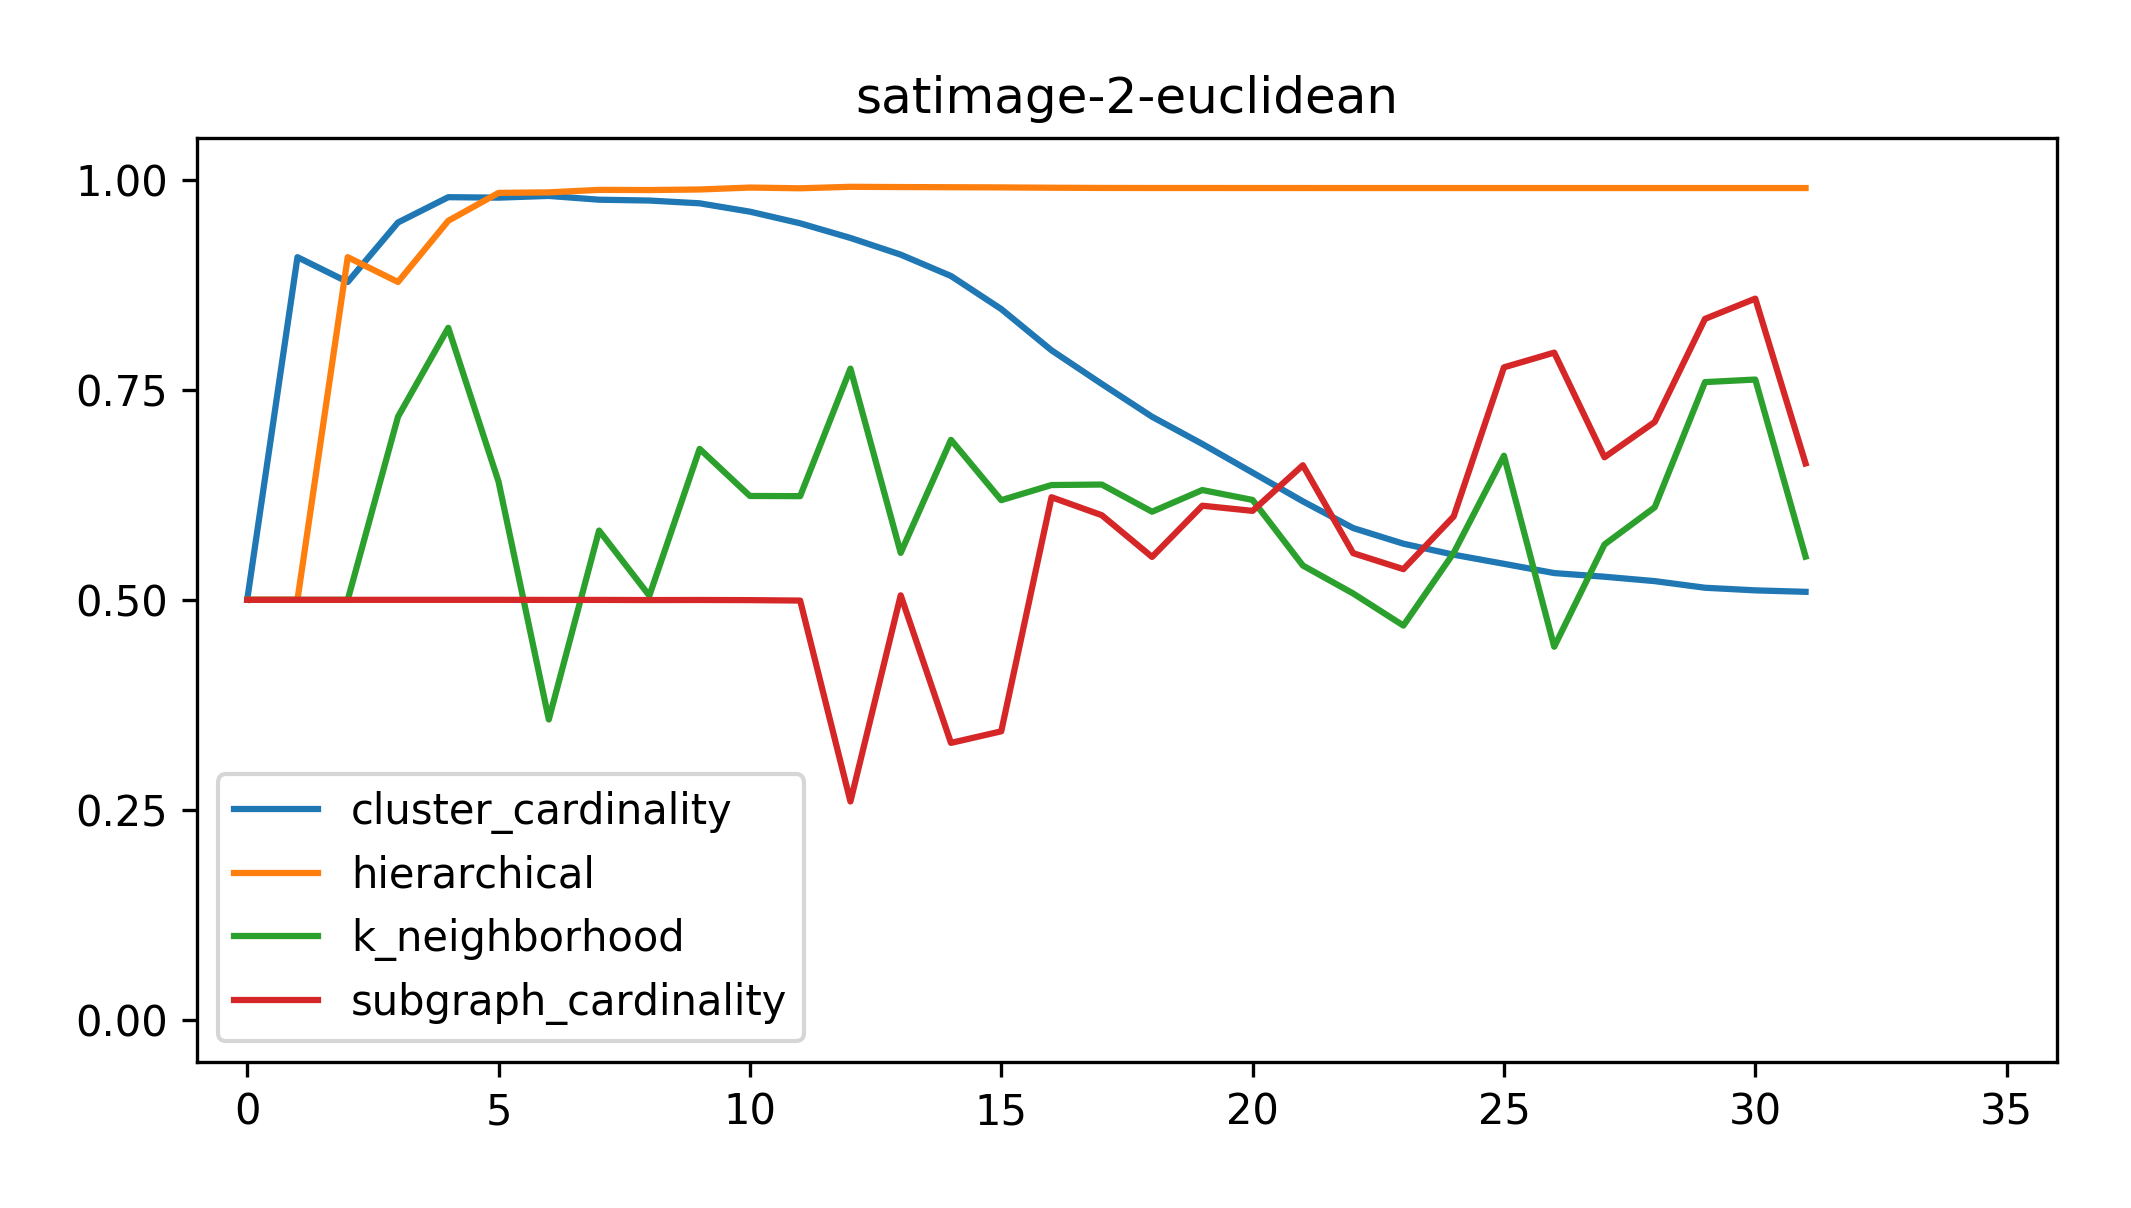
\includegraphics[width=2.2in]{kdd/static/auc_vs_depth/satimage-2-euclidean.png}
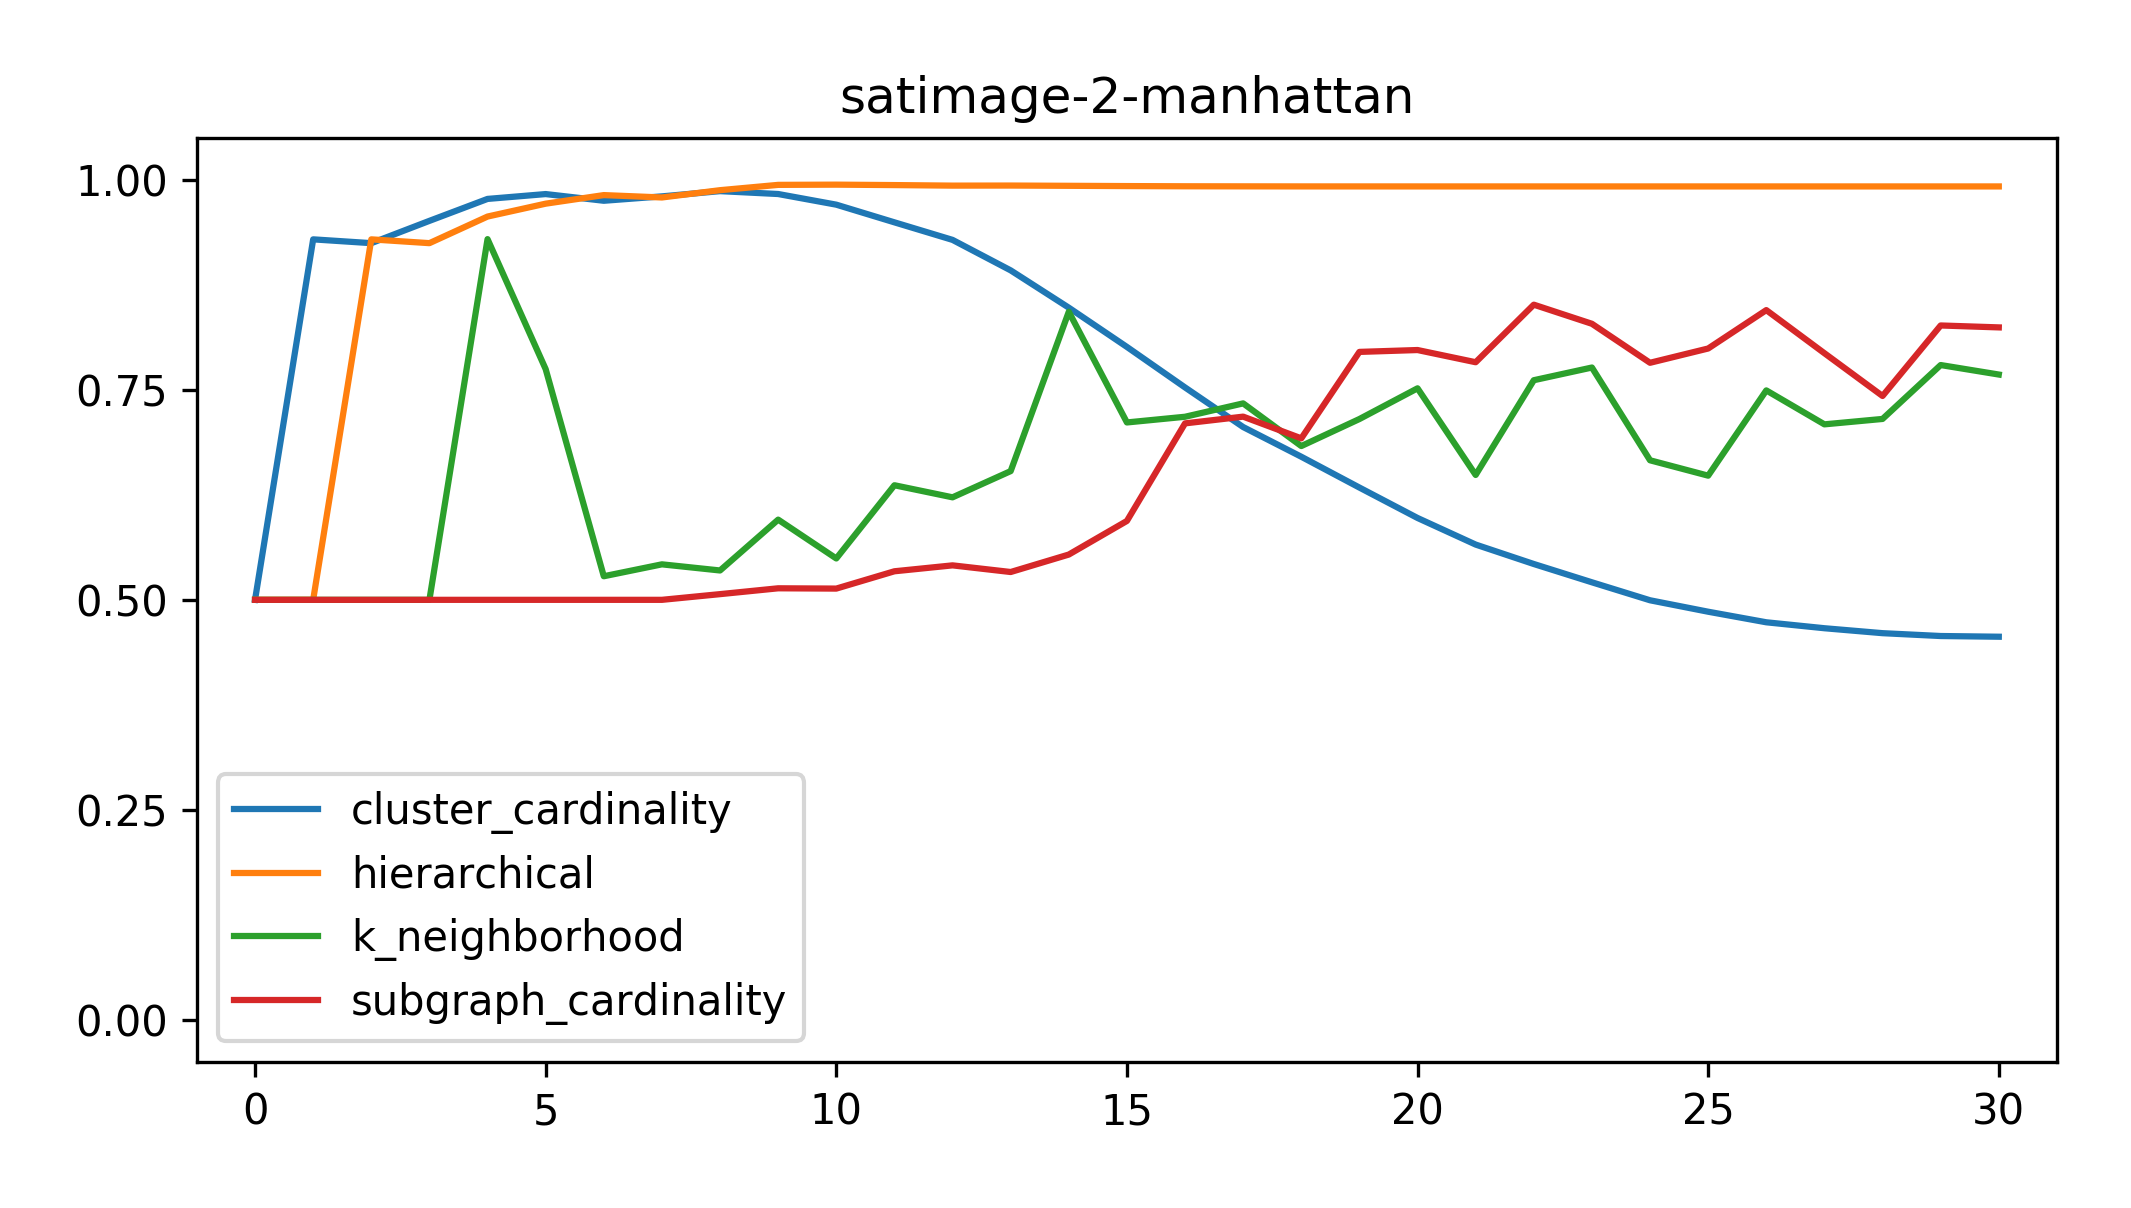
\includegraphics[width=2.2in]{kdd/static/auc_vs_depth/satimage-2-manhattan.png}

% Thyroid
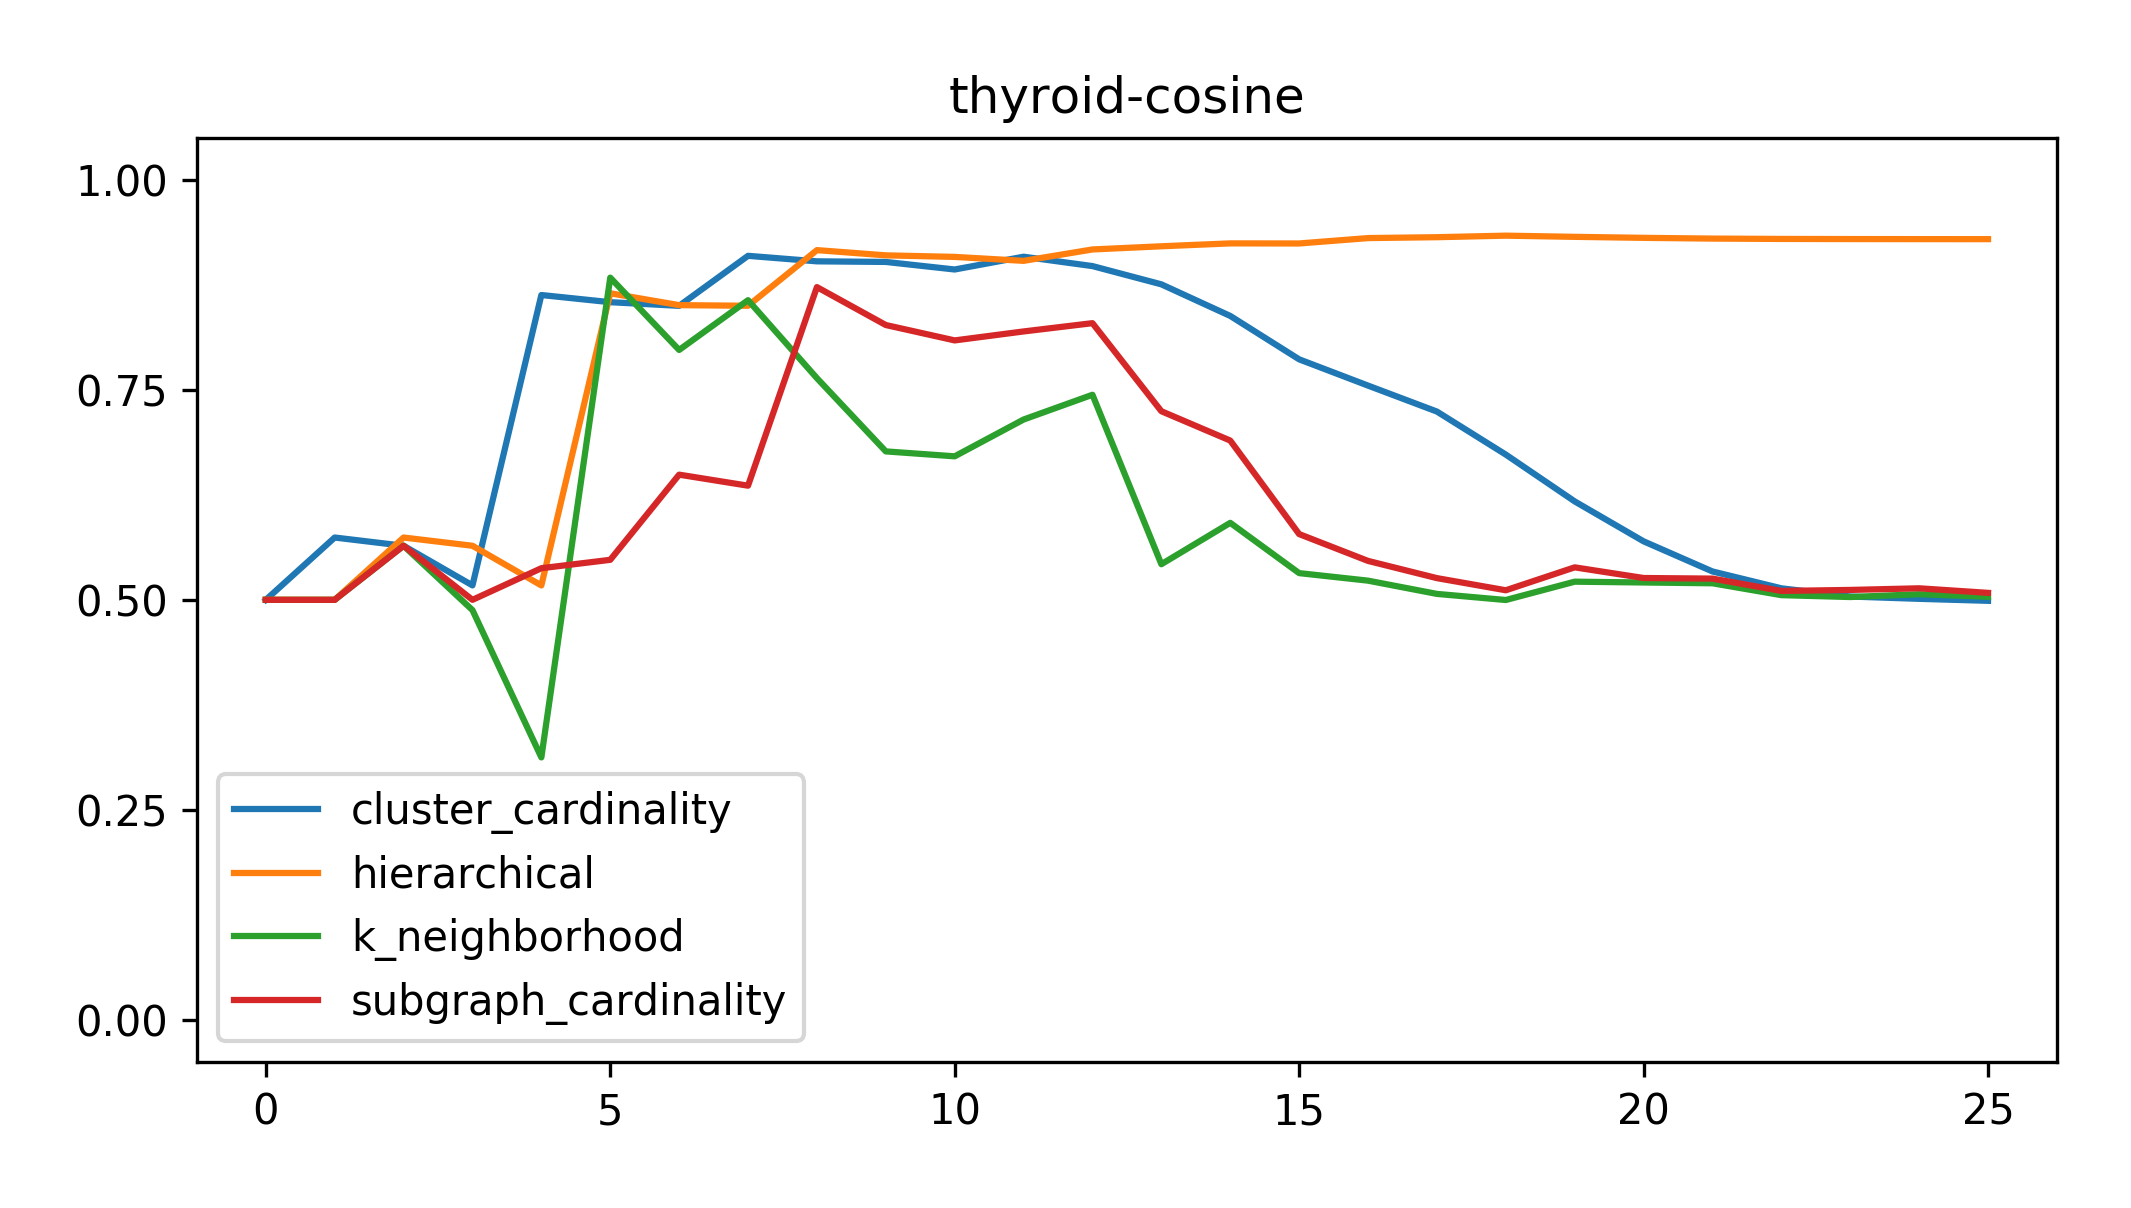
\includegraphics[width=2.2in]{kdd/static/auc_vs_depth/thyroid-cosine.png}
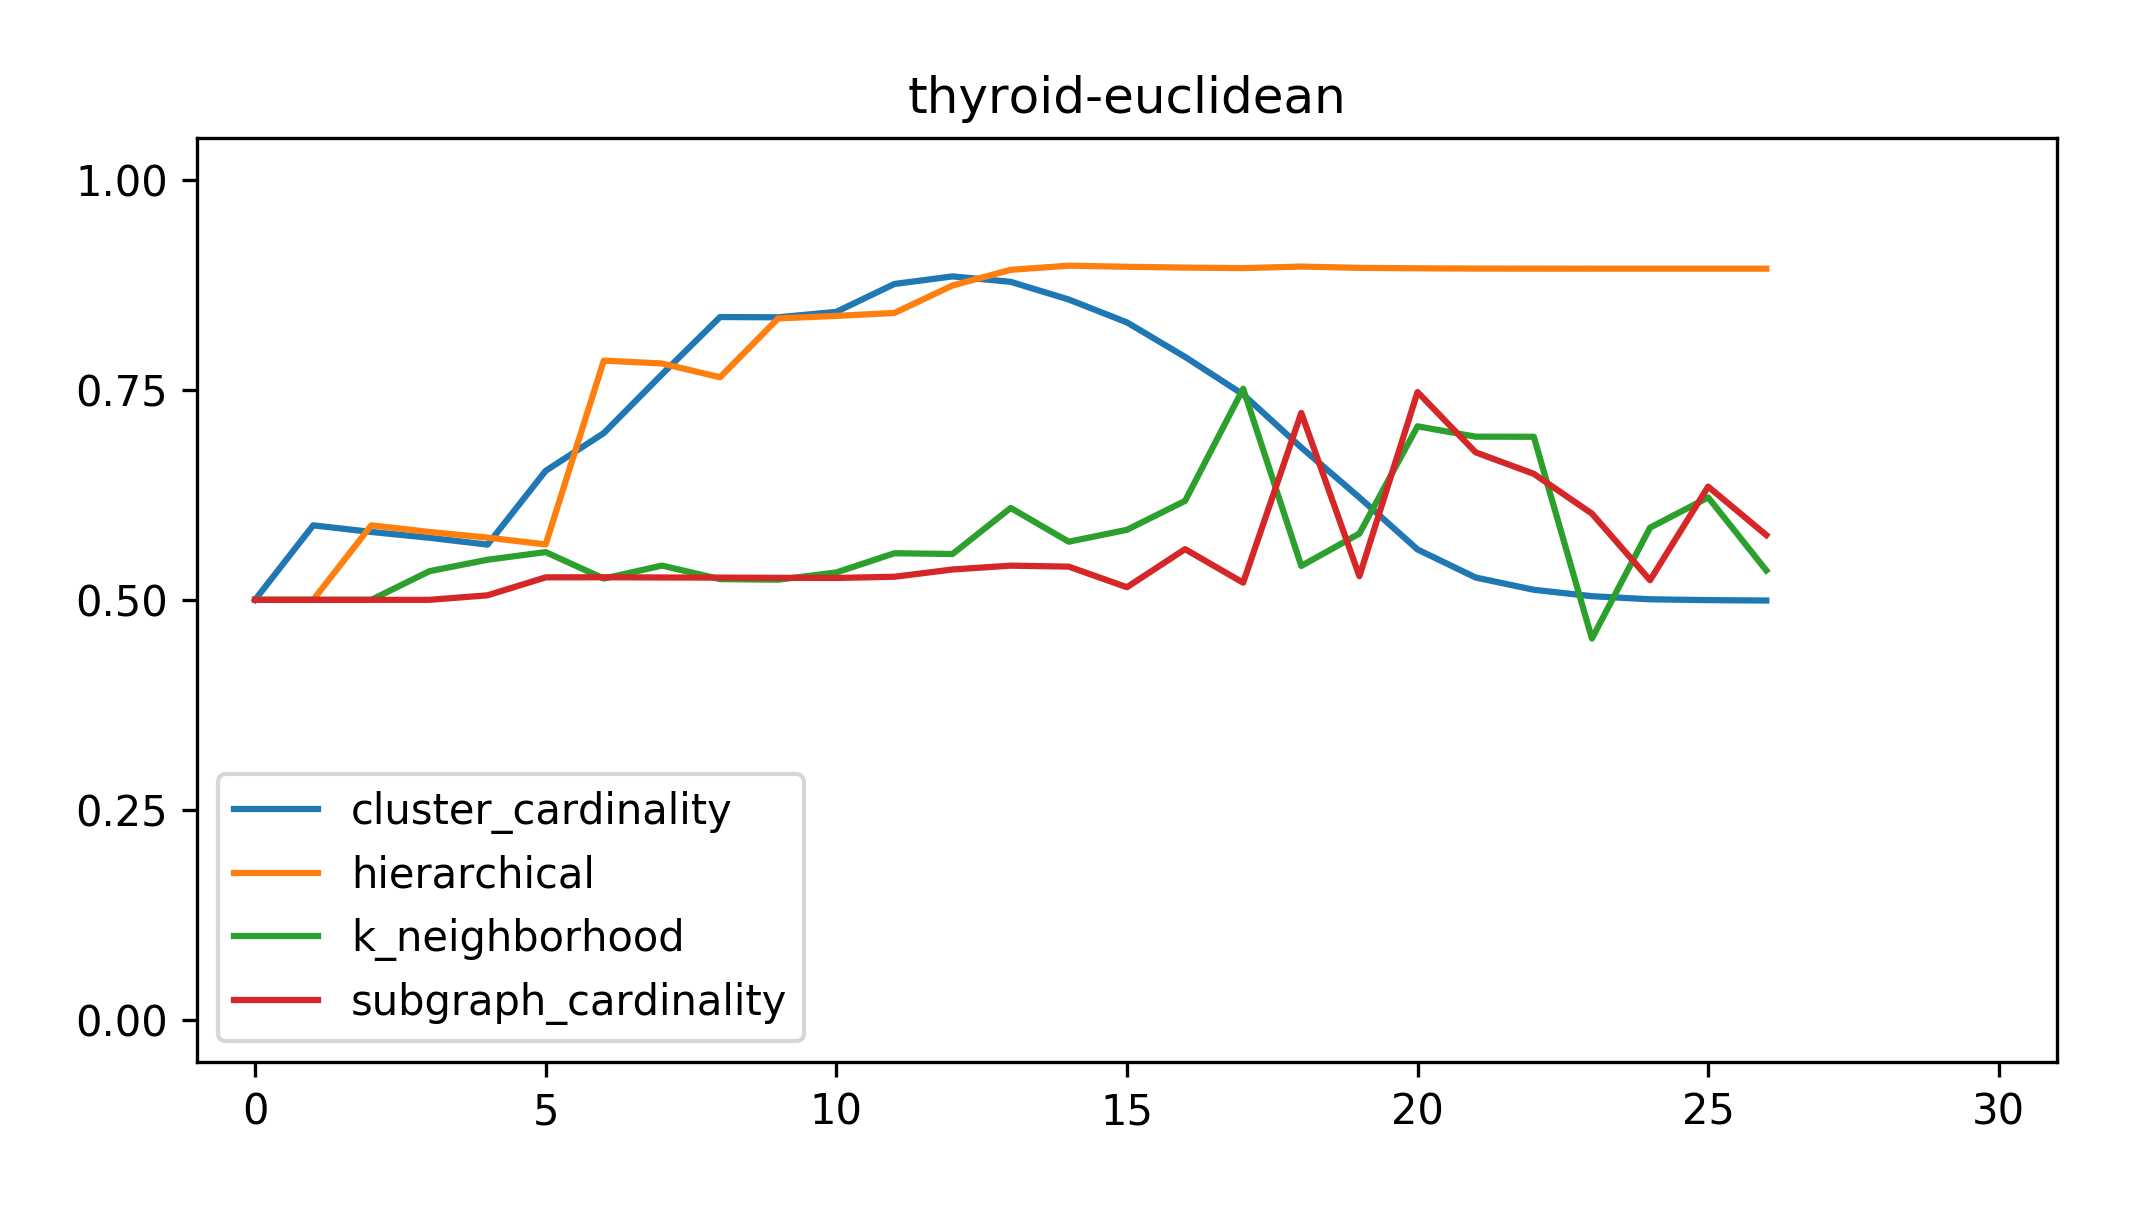
\includegraphics[width=2.2in]{kdd/static/auc_vs_depth/thyroid-euclidean.png}
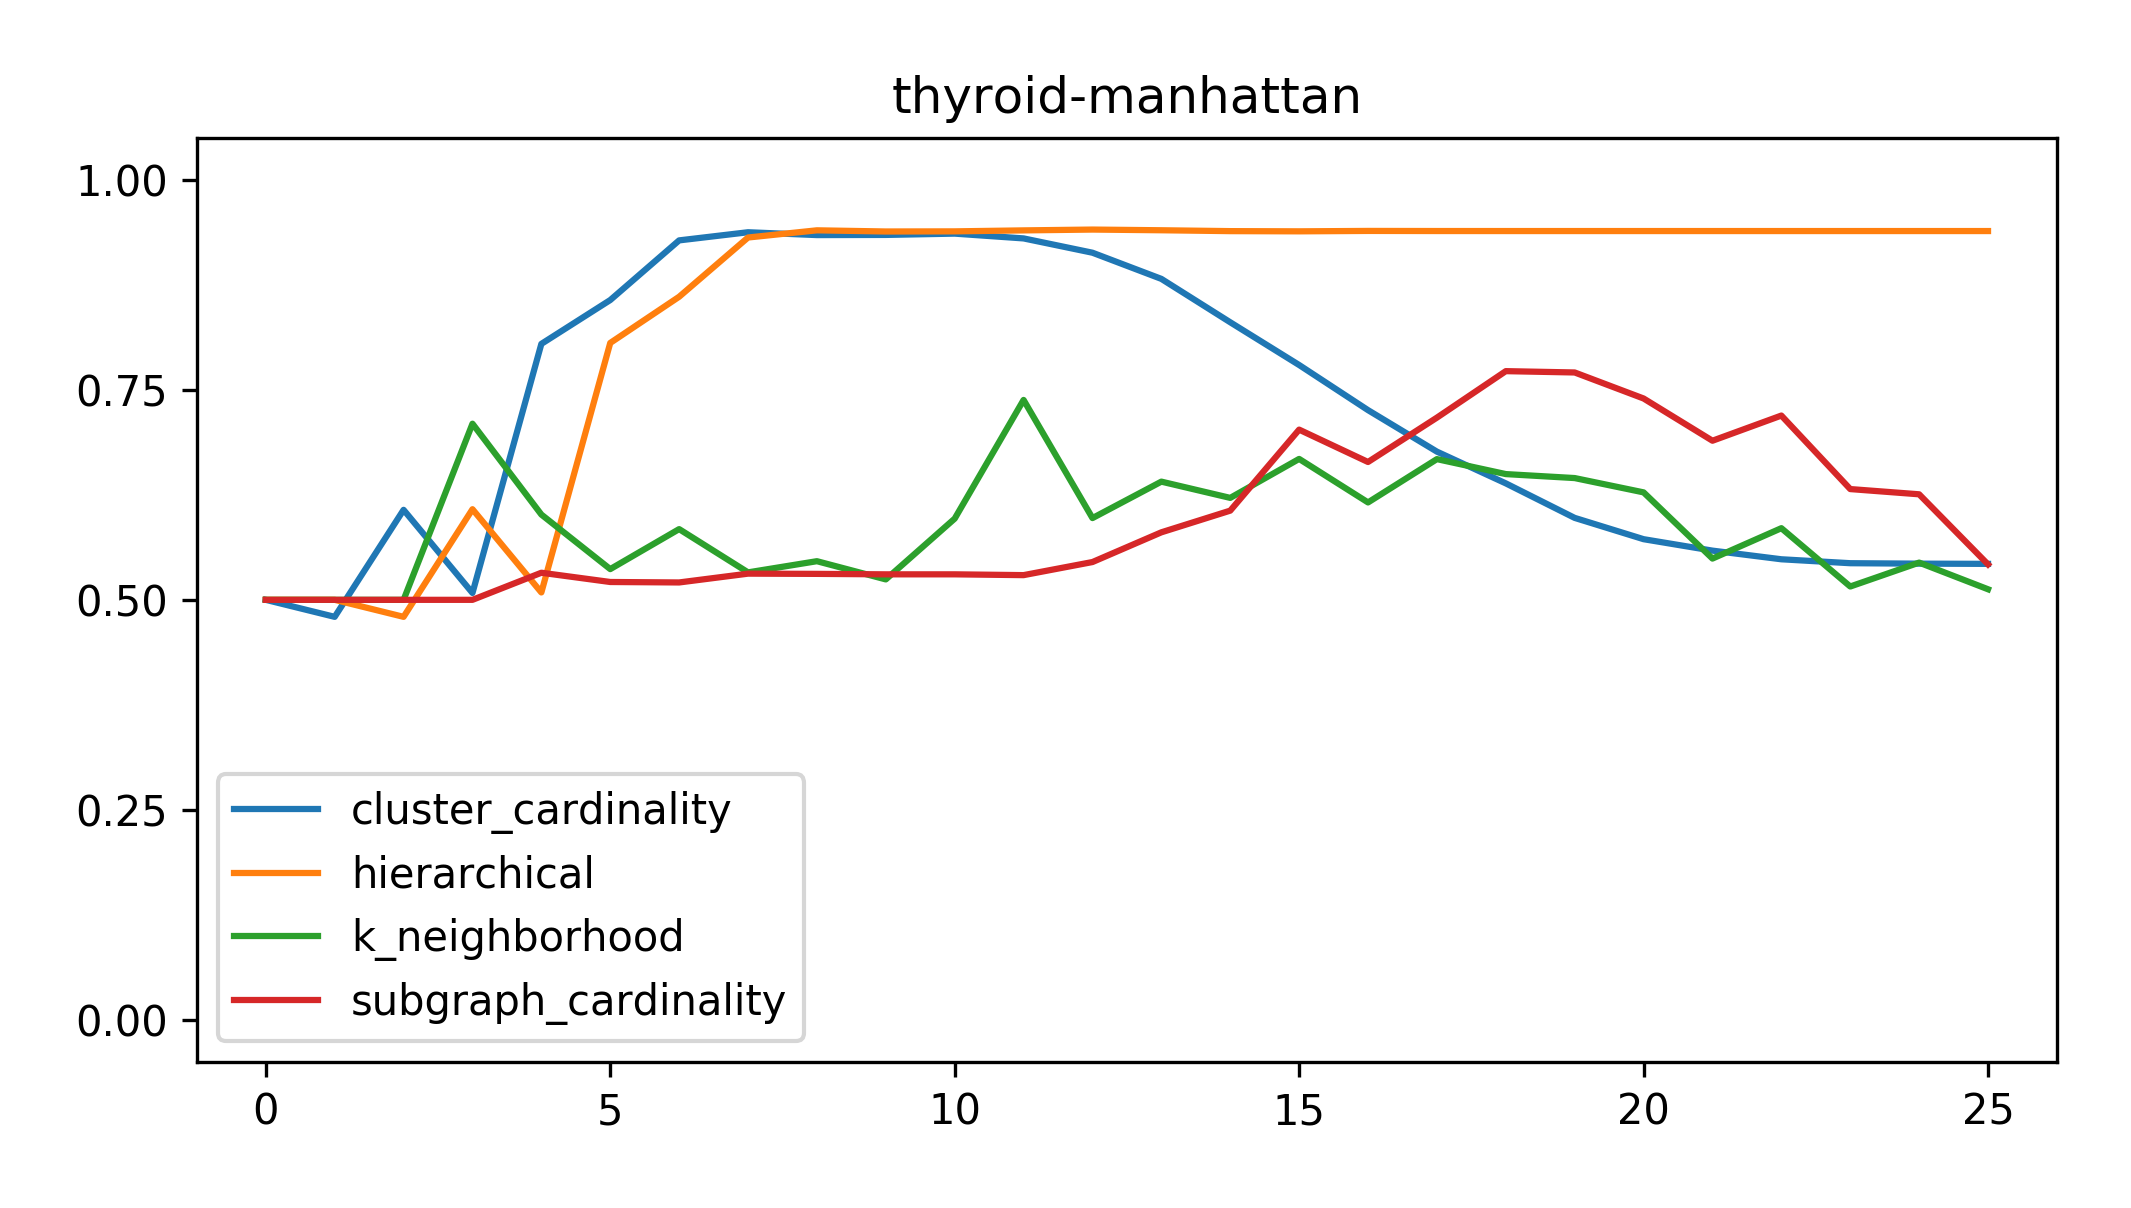
\includegraphics[width=2.2in]{kdd/static/auc_vs_depth/thyroid-manhattan.png}

% Vertebral
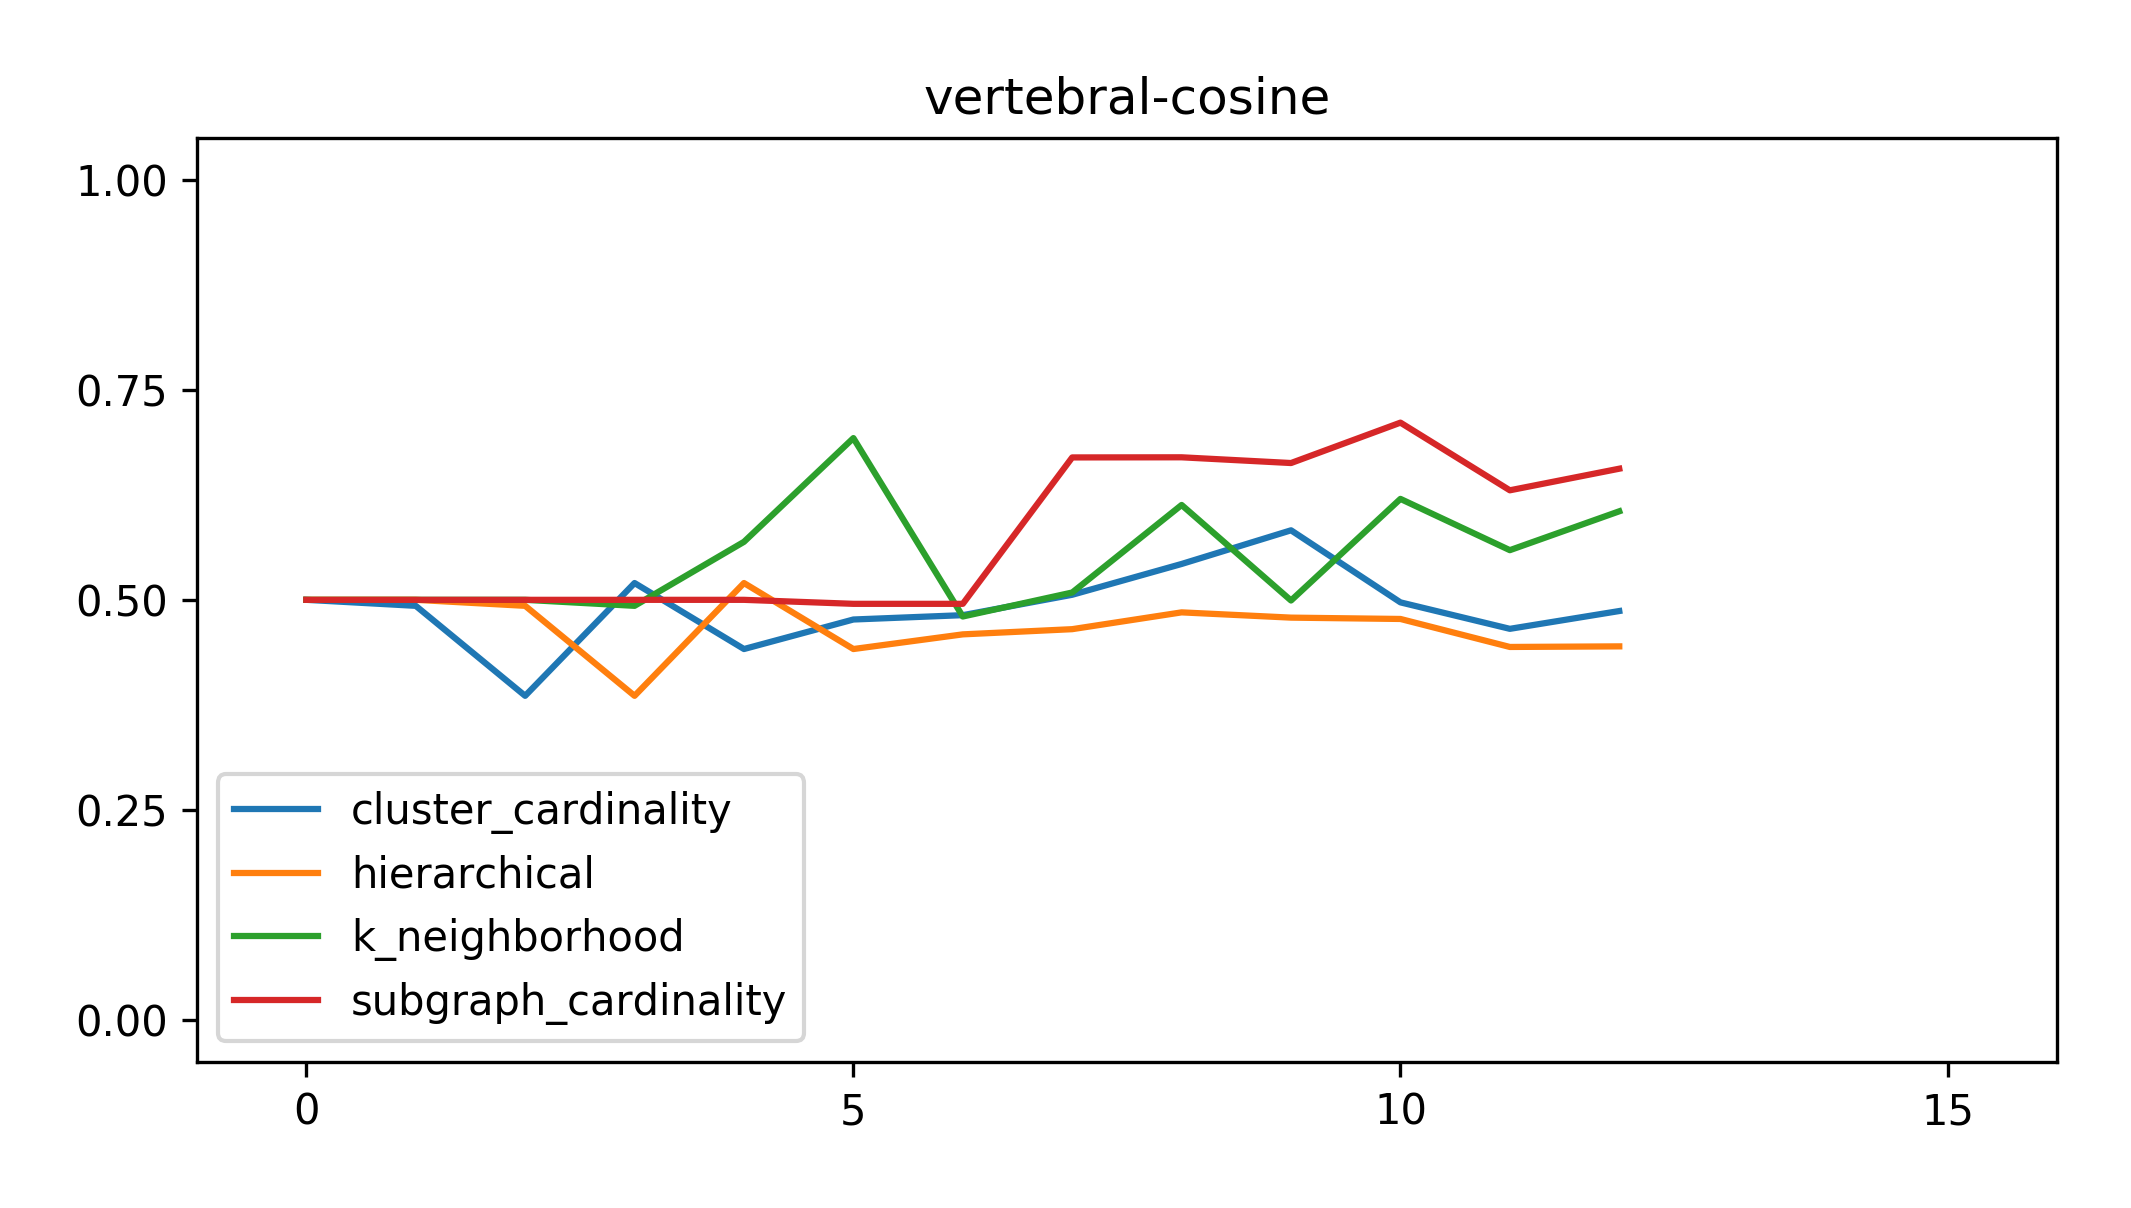
\includegraphics[width=2.2in]{kdd/static/auc_vs_depth/vertebral-cosine.png}
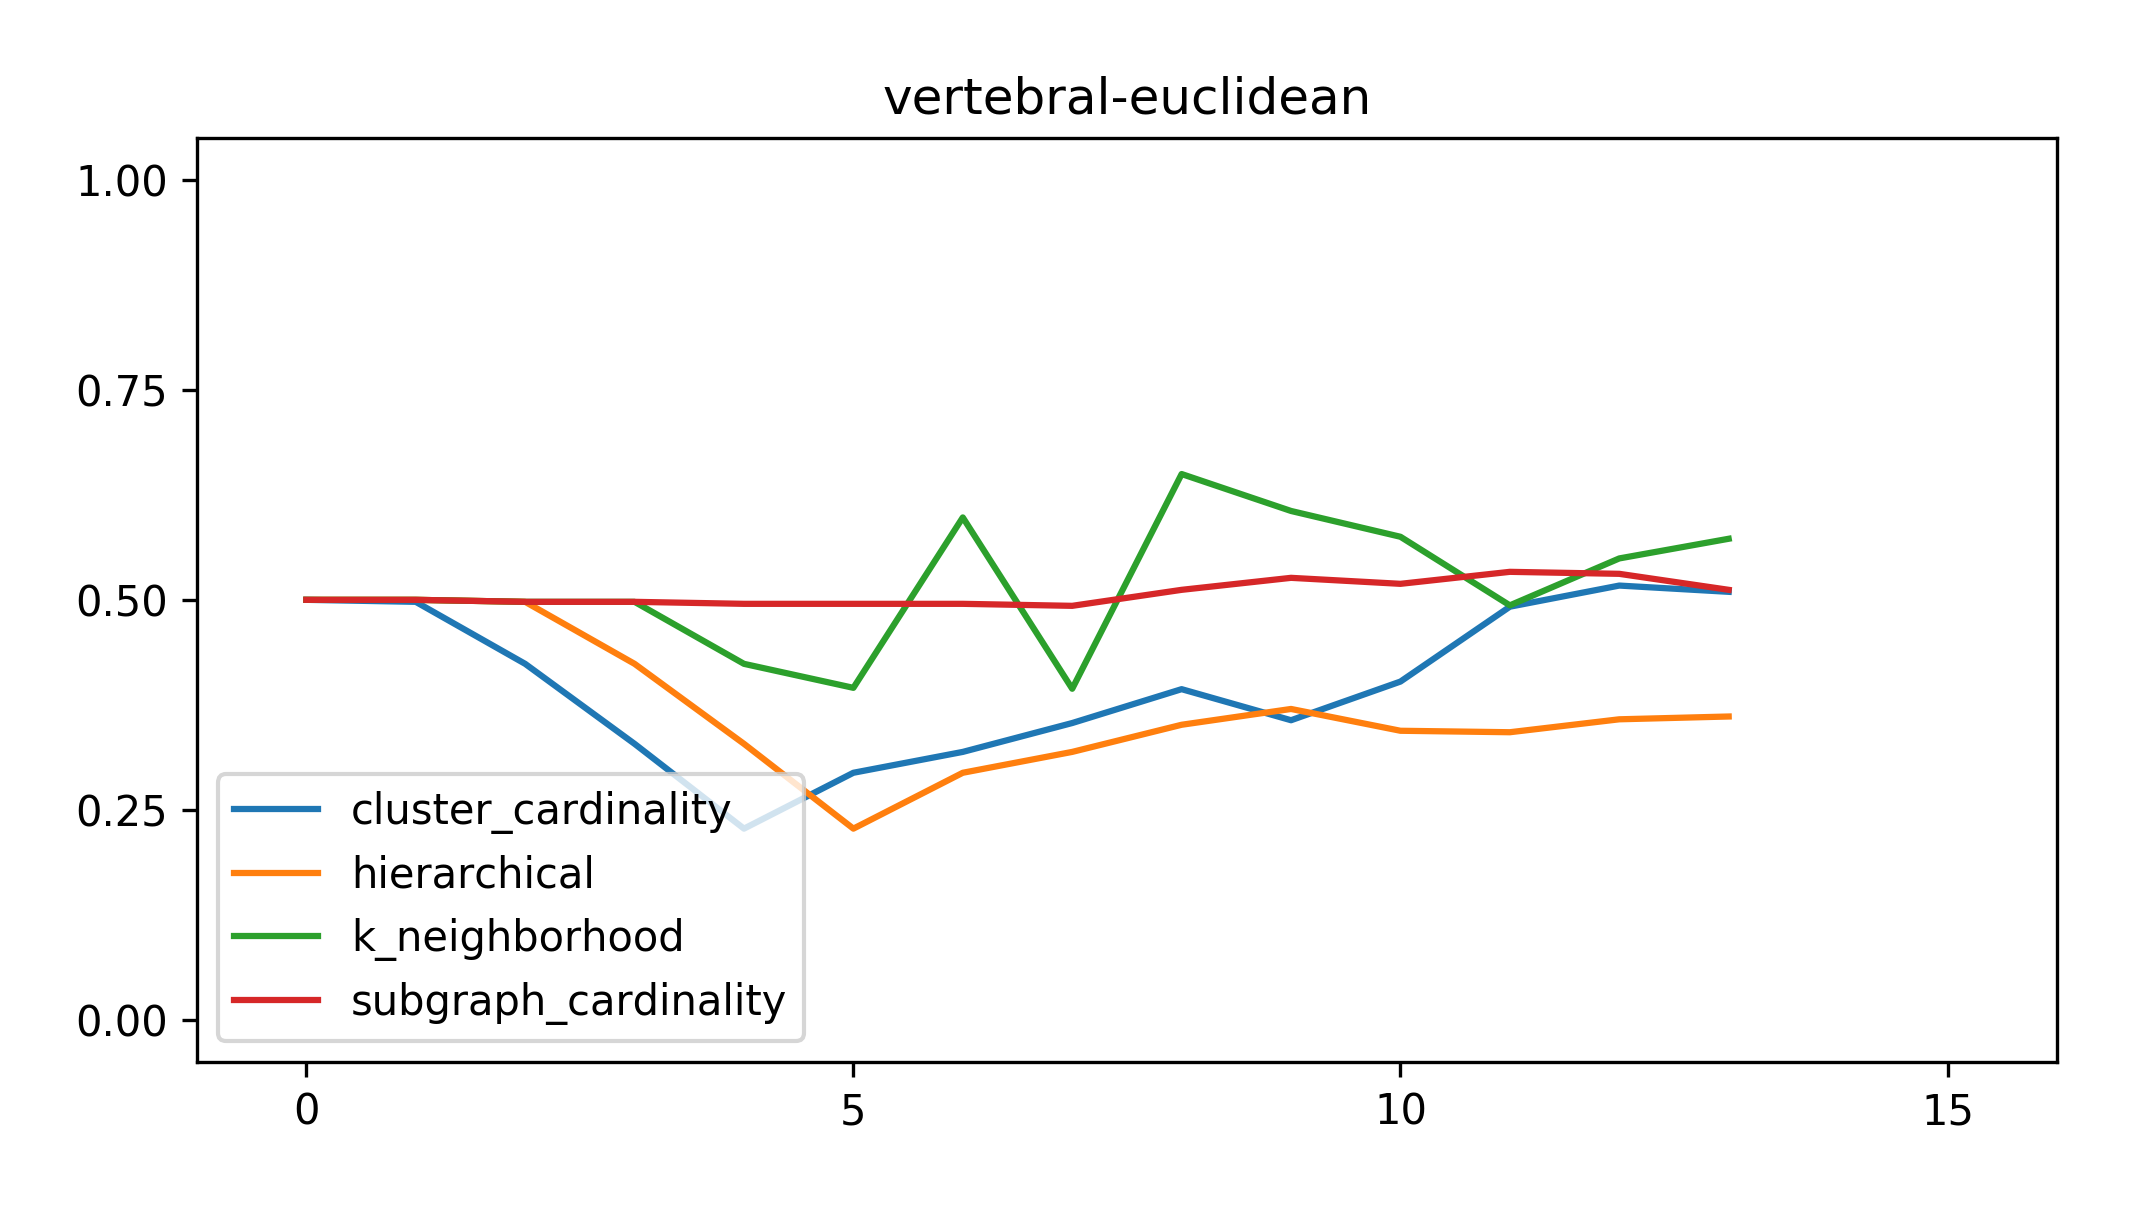
\includegraphics[width=2.2in]{kdd/static/auc_vs_depth/vertebral-euclidean.png}
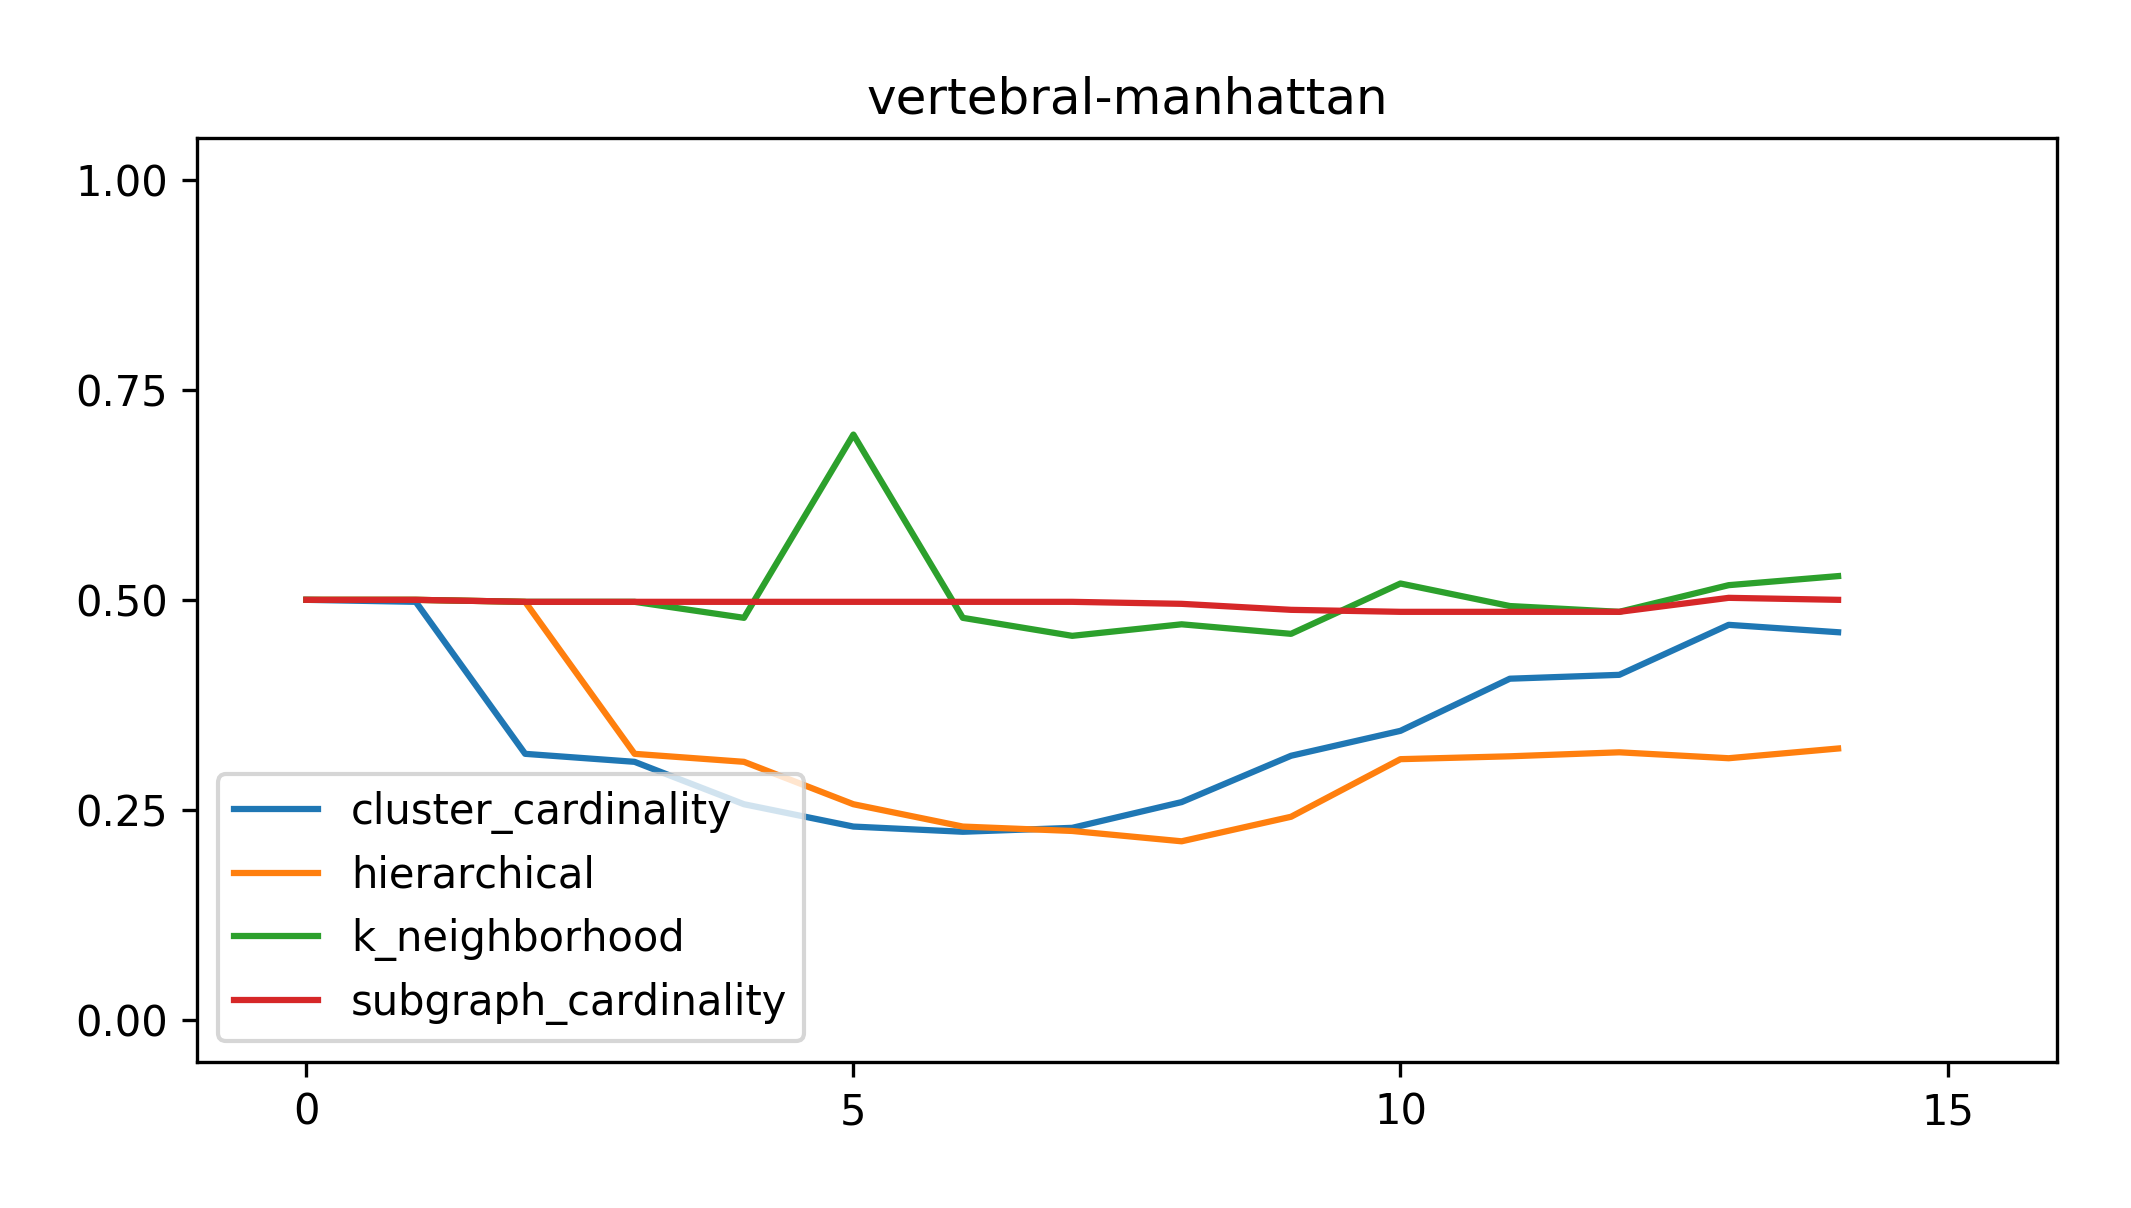
\includegraphics[width=2.2in]{kdd/static/auc_vs_depth/vertebral-manhattan.png}

% Vowels
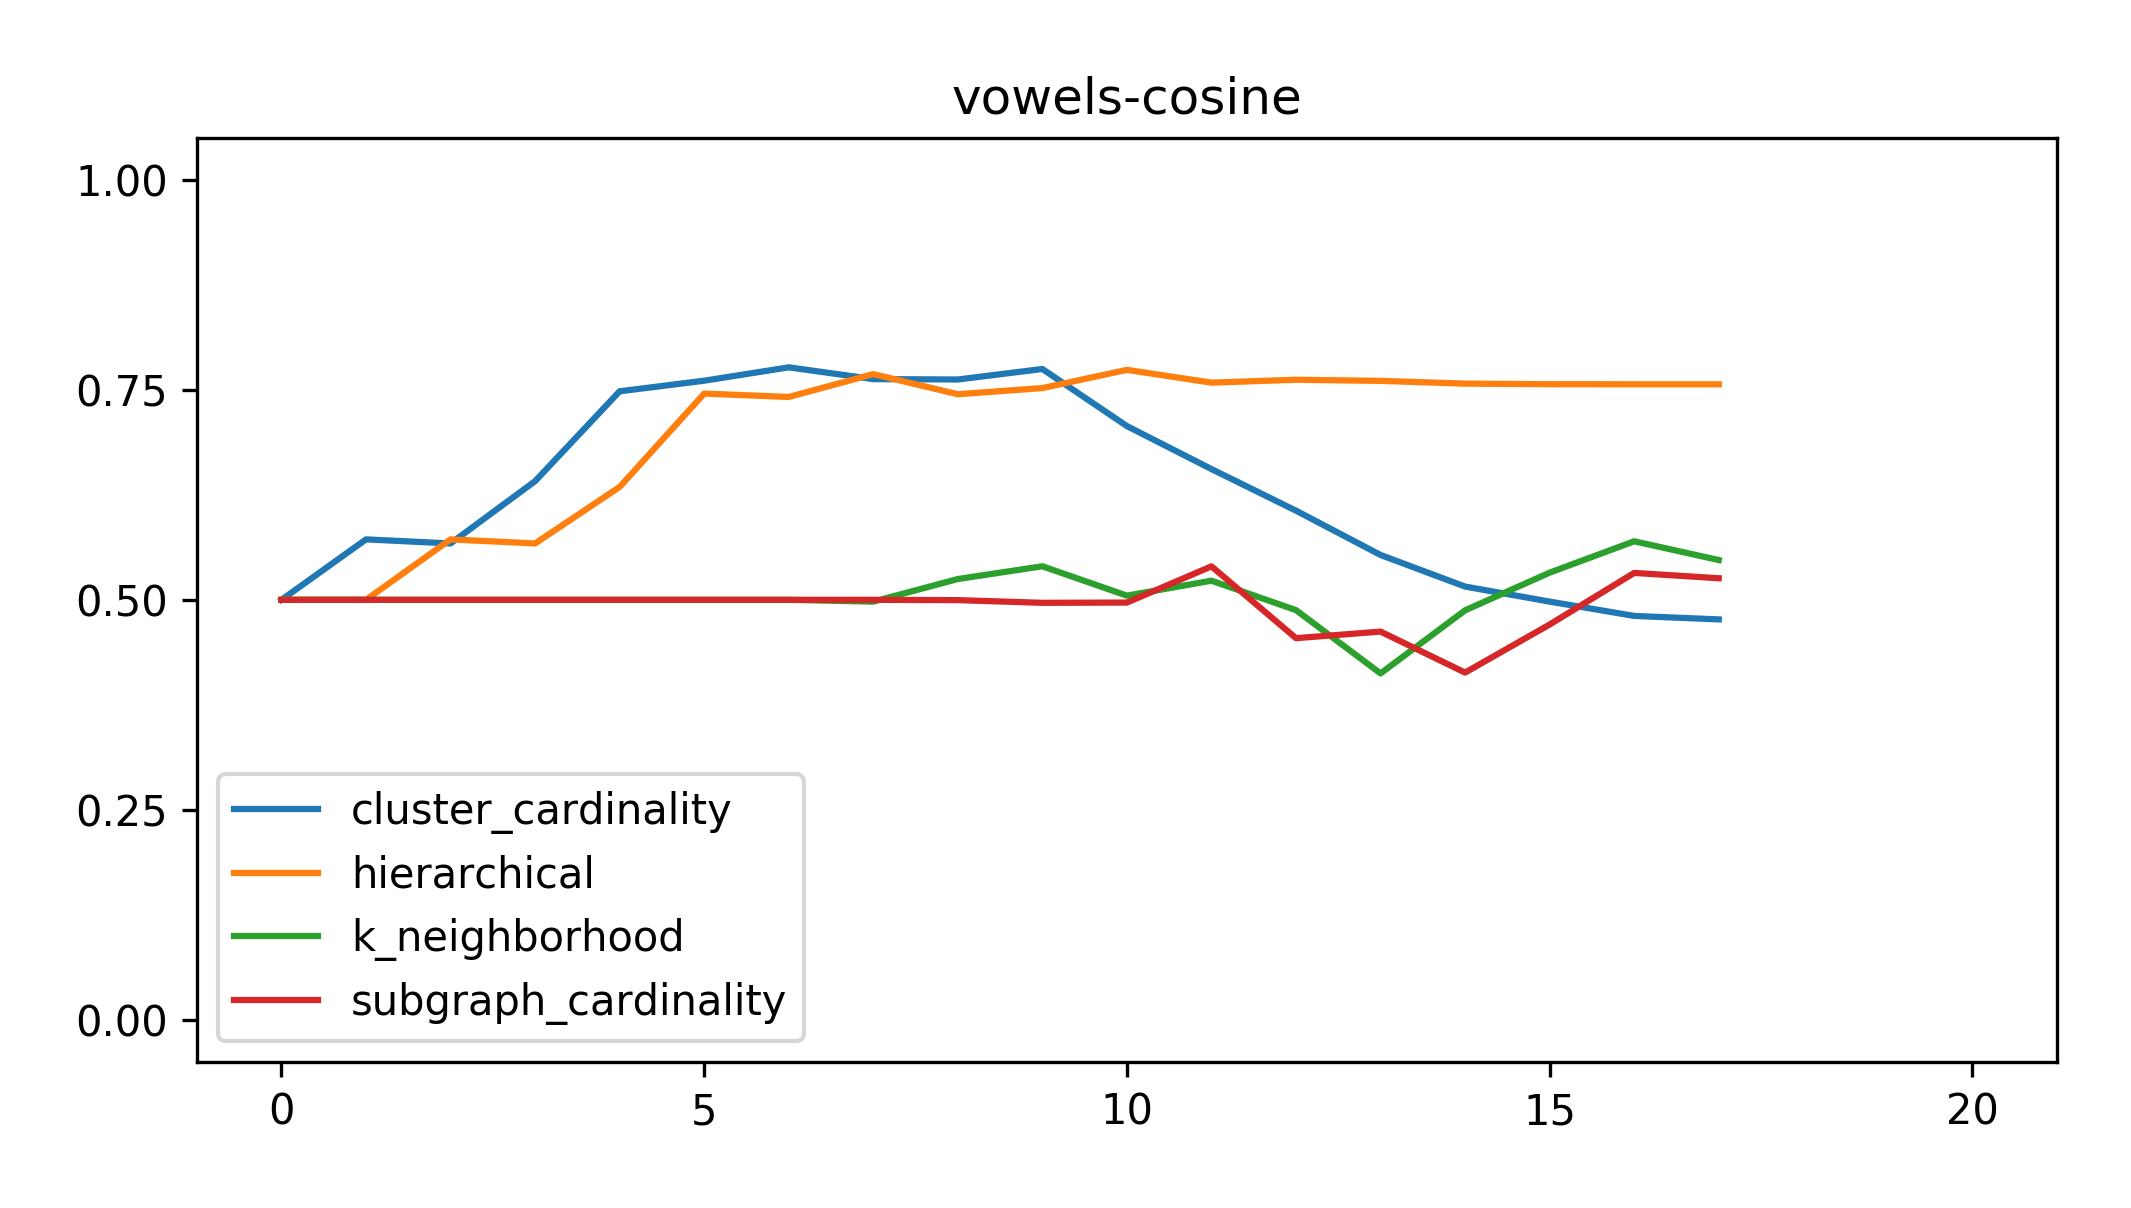
\includegraphics[width=2.2in]{kdd/static/auc_vs_depth/vowels-cosine.png}
\includegraphics[width=2.2in]{kdd/static/auc_vs_depth/vowels-euclidean.png}
\includegraphics[width=2.2in]{kdd/static/auc_vs_depth/vowels-manhattan.png}

% WBC
\includegraphics[width=2.2in]{kdd/static/auc_vs_depth/wbc-cosine.png}
\includegraphics[width=2.2in]{kdd/static/auc_vs_depth/wbc-euclidean.png}
\includegraphics[width=2.2in]{kdd/static/auc_vs_depth/wbc-manhattan.png}

% Wine
\includegraphics[width=2.2in]{kdd/static/auc_vs_depth/wine-cosine.png}
\includegraphics[width=2.2in]{kdd/static/auc_vs_depth/wine-euclidean.png}
\includegraphics[width=2.2in]{kdd/static/auc_vs_depth/wine-manhattan.png}

% HTTP
\includegraphics[width=2.2in]{kdd/static/auc_vs_depth/http-cosine.png}
\includegraphics[width=2.2in]{kdd/static/auc_vs_depth/http-euclidean.png}
\includegraphics[width=2.2in]{kdd/static/auc_vs_depth/http-manhattan.png}

\caption{
Plots of ROC-AUC vs Depth for our mearures of Anomolousness.
}

\label{results:datasets_3}
\end{figure*}

\begin{figure*}[!t]
\centering
% SMTP
\includegraphics[width=2.2in]{kdd/static/auc_vs_depth/smtp-cosine.png}
\includegraphics[width=2.2in]{kdd/static/auc_vs_depth/smtp-euclidean.png}
\includegraphics[width=2.2in]{kdd/static/auc_vs_depth/smtp-manhattan.png}

% Pendigits
\includegraphics[width=2.2in]{kdd/static/auc_vs_depth/pendigits-cosine.png}
\includegraphics[width=2.2in]{kdd/static/auc_vs_depth/pendigits-euclidean.png}
\includegraphics[width=2.2in]{kdd/static/auc_vs_depth/pendigits-manhattan.png}

% Mammography
\includegraphics[width=2.2in]{kdd/static/auc_vs_depth/mammography-cosine.png}
\includegraphics[width=2.2in]{kdd/static/auc_vs_depth/mammography-euclidean.png}
\includegraphics[width=2.2in]{kdd/static/auc_vs_depth/mammography-manhattan.png}

\caption{
Plots of ROC-AUC vs Depth for our mearures of Anomolousness.
}

\label{results:datasets_4}
\end{figure*}


\section{Discussion}
\label{sec:conclusions}

We have presented CHAODA (Clustered Hierarchical Anomaly and Outlier Detection Algorithms), a collection of five algorithms that exploit properties of a hierarchical cluster tree which represents an approximate manifold in $n$-dimensional space.
All five algorithms are trivial to implement on top of the manifold-learning framework we call CLAM (Clustered Learning of Approximate Manifolds); CHAODA builds on this framework similarly to CHESS~\cite{ishaq2019entropy}, which learns a manifold in the same way, but for the purpose of accelerating approximate search.
In CHESS, the geometric and topological properties of low fractal dimension and low metric entropy are advantages; indeed, CHESS does not perform particularly well if those properties are not present.
CHAODA, on the other hand, while competitive with other state-of-the-art anomaly-detection approaches on ``easy'' data sets (we define as \textit{easy} any data set where a one-class SVM performs well), outperforms other current methods when the data exhibit precisely those properties that CHESS depends on for acceleration. In particular, CHAODA outperforms other approaches on high-dimensional data sets, with the exception of the highest-dimensional dataset analyzed, ``annthyroid,'' where iForest and AOD perform better.

% note: make sure the above statement is actually true! Need to look at t-SNE and UMAP 
% for the breast cancer data set, as well as fractal dimension

\begin{figure}
    \centering
    % TODO!!
    \includegraphics{kdd/static/auc_vs_depth/annthyroid-cosine.png}
    \caption{UMAP of Annthyroid Dataset}
    \label{fig:annthyroid-umap}
\end{figure}

With the sole exception of the annthyroid dataset, the algorithms presented here outperform or match all other approaches. 
At this point, it is important that we discuss some of the reasons that may be contributing to CHAODA's difficulty with this one dataset in particular.
Upon further investigation, it appears that this data may be in too few dimensions for CLAM to partition it into a useful manifold.
In UMAP projections we created on annthyroid~\ref{fig:annthyroid-umap}, it can be clearly seen that the anomalous data appears to live directly on the manifold, with only a small pocket appearing to be distinctly off.
This aligns perfectly with our expectations for CHAODA.
Indeed, the manifold being both learnable and distinctly separate from the anomalous data are mandatory properties for any of our approaches to be effective.
Fortunately, we can clearly see that these properties are apparent in all other datasets studied.

One current limitation in CHAODA is that the depth of the cluster tree at which anomaly detection performs best is not the same for every data set, and thus our results could be seen as ``cherry-picking'' from a scattershot approach.
This is because as depth increases, the induced graph ``shatters'', i.e. the number of components in the graph approaches the number of clusters in the graph.
Future work should certainly explore optimal stopping criteria so that we can automate stopping just before the graph shatters.
However, as shown in Figure~\ref{}, for most datasets, performance is not overly sensitive to the choice of depth.
We can treat depth as a hyperparameter to all of the methods described, but a detailed analysis of possible criteria for determining the optimal depth is essential future work.

% TODO: Need to look at local fractal dimension, or volume ratios, vs. optimal depth. Ideally we can say something like:
% The strong correlation between local fractal dimension and optimal tree depth suggests a guideline for determining an optimal tree depth directly from the data.

The choice of distance function also has a significant impact on anomaly-detection performance.
In this case, domain knowledge is likely the best way to determine the distance function of choice.
In future work, we seek to explore a more diverse collection of domain-appropriate distance functions, such as Wasserstein distance on images, and Levenshtein edit distance on strings. 

% TODO: Have we proved this?
% Say something about applying CHAODA for inputs to an ANN, in particular detecting just-off-manifold malicious inputs, like the school bus / ostrich example.

In conclusion, we have demonstrated that by learning approximate manifolds, we can exploit the embedded knowledge to implement trivial algorithms capable of outperforming other state-of-the-art approaches to anomaly detection.

\section{Acknowledgements}
\label{sec:acknowledgements}

We have been Clearly Hoping that Our Work Detects Anomalies.


\bibliographystyle{ACM-Reference-Format}
\bibliography{references}
\end{document}
